% Copyright (c) 2014,2016 Casper Ti. Vector
% Public domain.
\chapter{$Z_{cs}$ states in $\Bp\to\jpsi\phi\Kp$ decay}
\label{app:Zcs_appendix}
%\pkuthssffaq % 中文测试文字。


\section{Angular moments}
\label{sec:app:Y}

The unnormalized Legendre moments defined as
\begin{equation}
<P^U_{\ell}>=\sum_{i=1}^{N_{\rm events}}\frac{1}{\epsilon_i}P_{\ell}(\cos\theta),
\end{equation}
where $P_{\ell}(\cos\theta)$ is the Legendre polynomial of order $\ell$ and $\epsilon_i$ is the efficiency for each event, 
depending on its phase-space location.
Structures related to a spin $J$ resonance described by the helicity angle $\theta$, 
can show up in the Legendre moments of rank up to $l=2J$, 
or up to $l=J+J'$ in interferences of $J$ and $J'$ amplitudes.  
Mass dependence of the Legendre moments can provide hints about resonances present in the data, 
since their quantum numbers restrict $J$ values. 
Unfortunately, 
reflections of decays from the other decay chain(s) can generate mass dependent variations of the moments at any rank, 
obscuring interpretation of the data.

The moments distribution is obtained by weighting each events by a weight $\frac{1}{\epsilon_i}P_{\ell}(\cos\theta)$. 
The background contribution in the data is subtracted, 
and the signal contribution is achieved as the moments distribution of events in the signal region minus the moments distribution of sideband events, 
the latter is scaled by the ratio of background yields between the signal and the sideband regions.
In Fig.~\ref{mom5phi}  we show the Legendre moments vs.~$\mjf$ using cosine helicity angle of $\jpsi\phi$ as the argument of the polynomial.
The nominal model describes the data reasonably well.
Improvements over the old Run 1 model are clearly visible in several moments.

In Fig.~\ref{mom5kst}, the Legendre moments vs.~$\mfk$
using cosine helicity angle of $\phi K$ are shown. 
The agreement is again reasonable, 
but the differences between the nominal and old Run 1 model are smaller.

The Legendre moments vs~$\mjk$ using cosine helicity angle of $\jpsi K$  are shown in Fig.~\ref{mom5z}. 
Some improvements of the nominal model as compared to the old Run 1 model are see.



\begin{figure}[htbp]
\centering
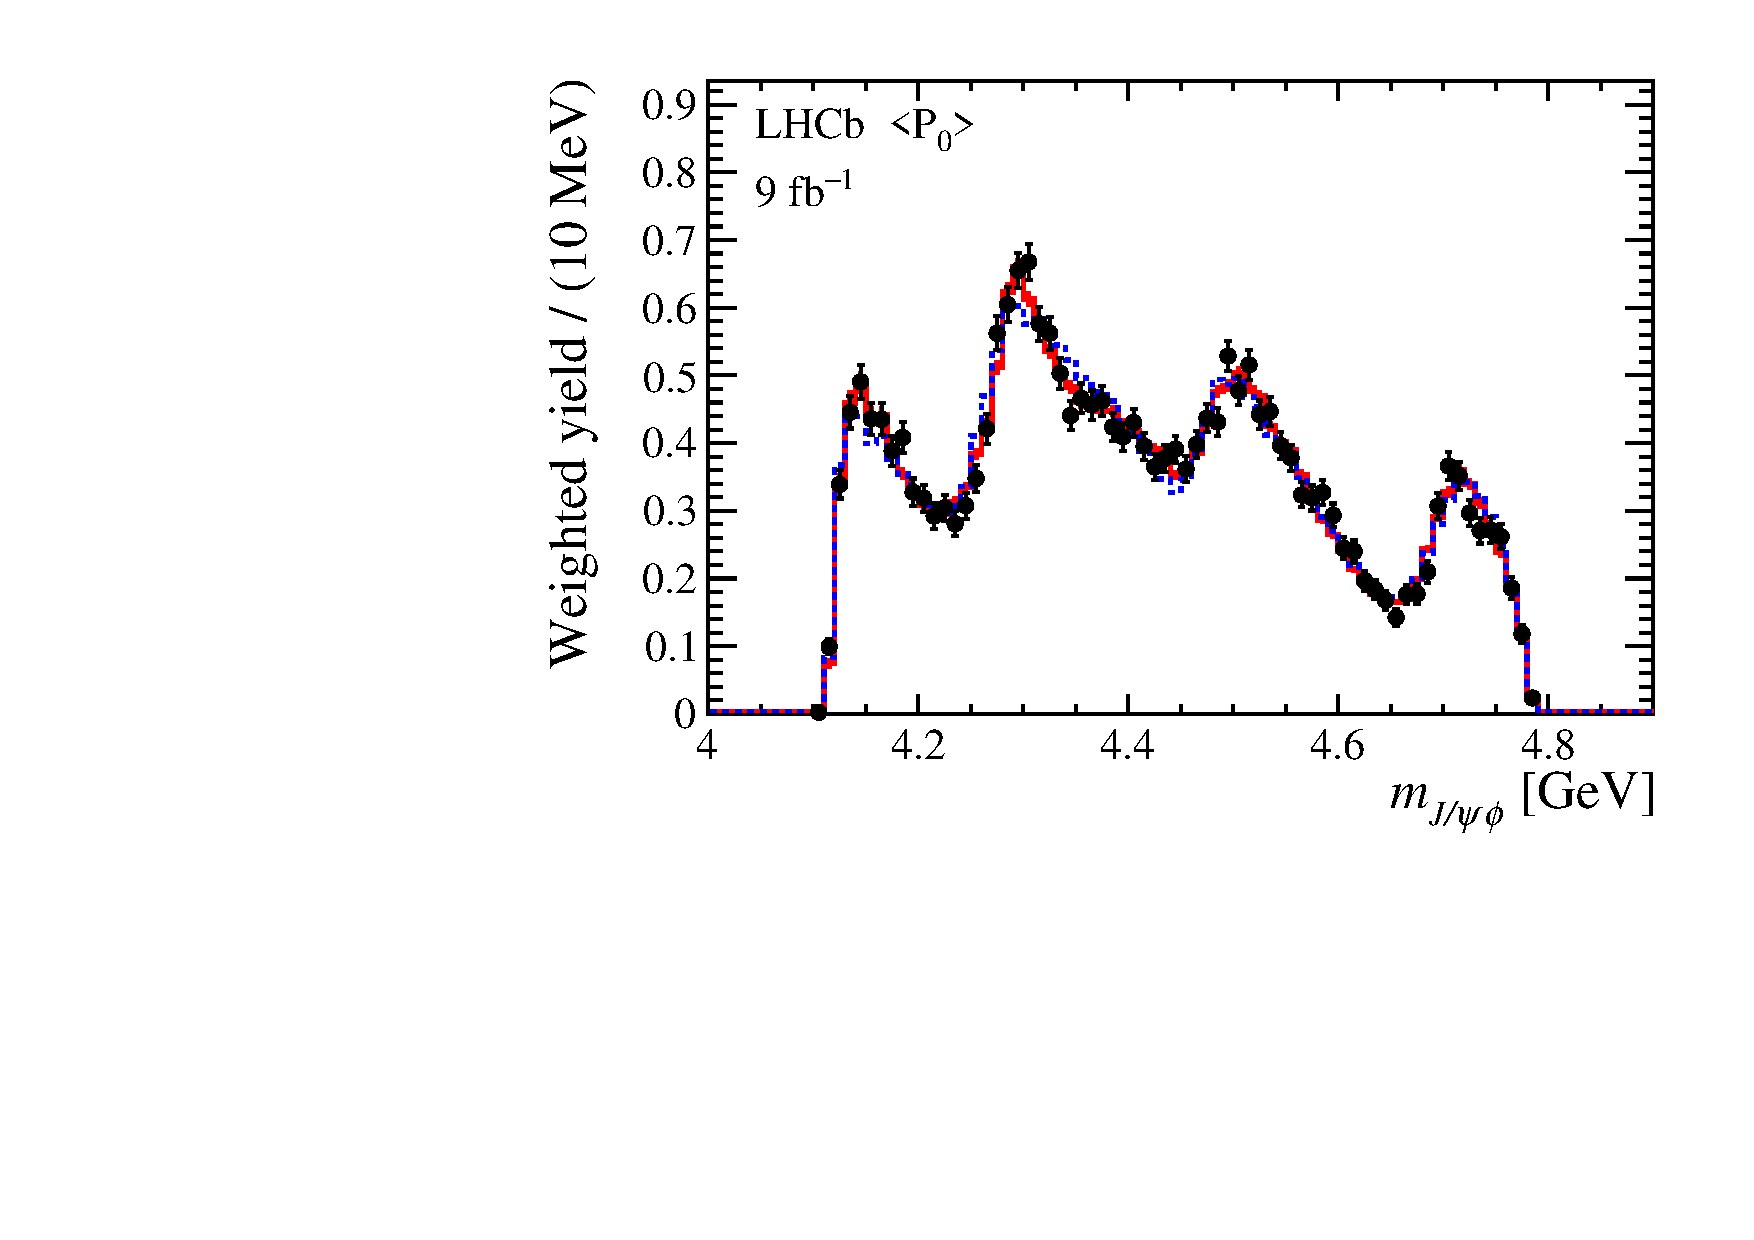
\includegraphics[width=0.33\textwidth]{Figures/03_Zcs/app_moments/shyphi0}%
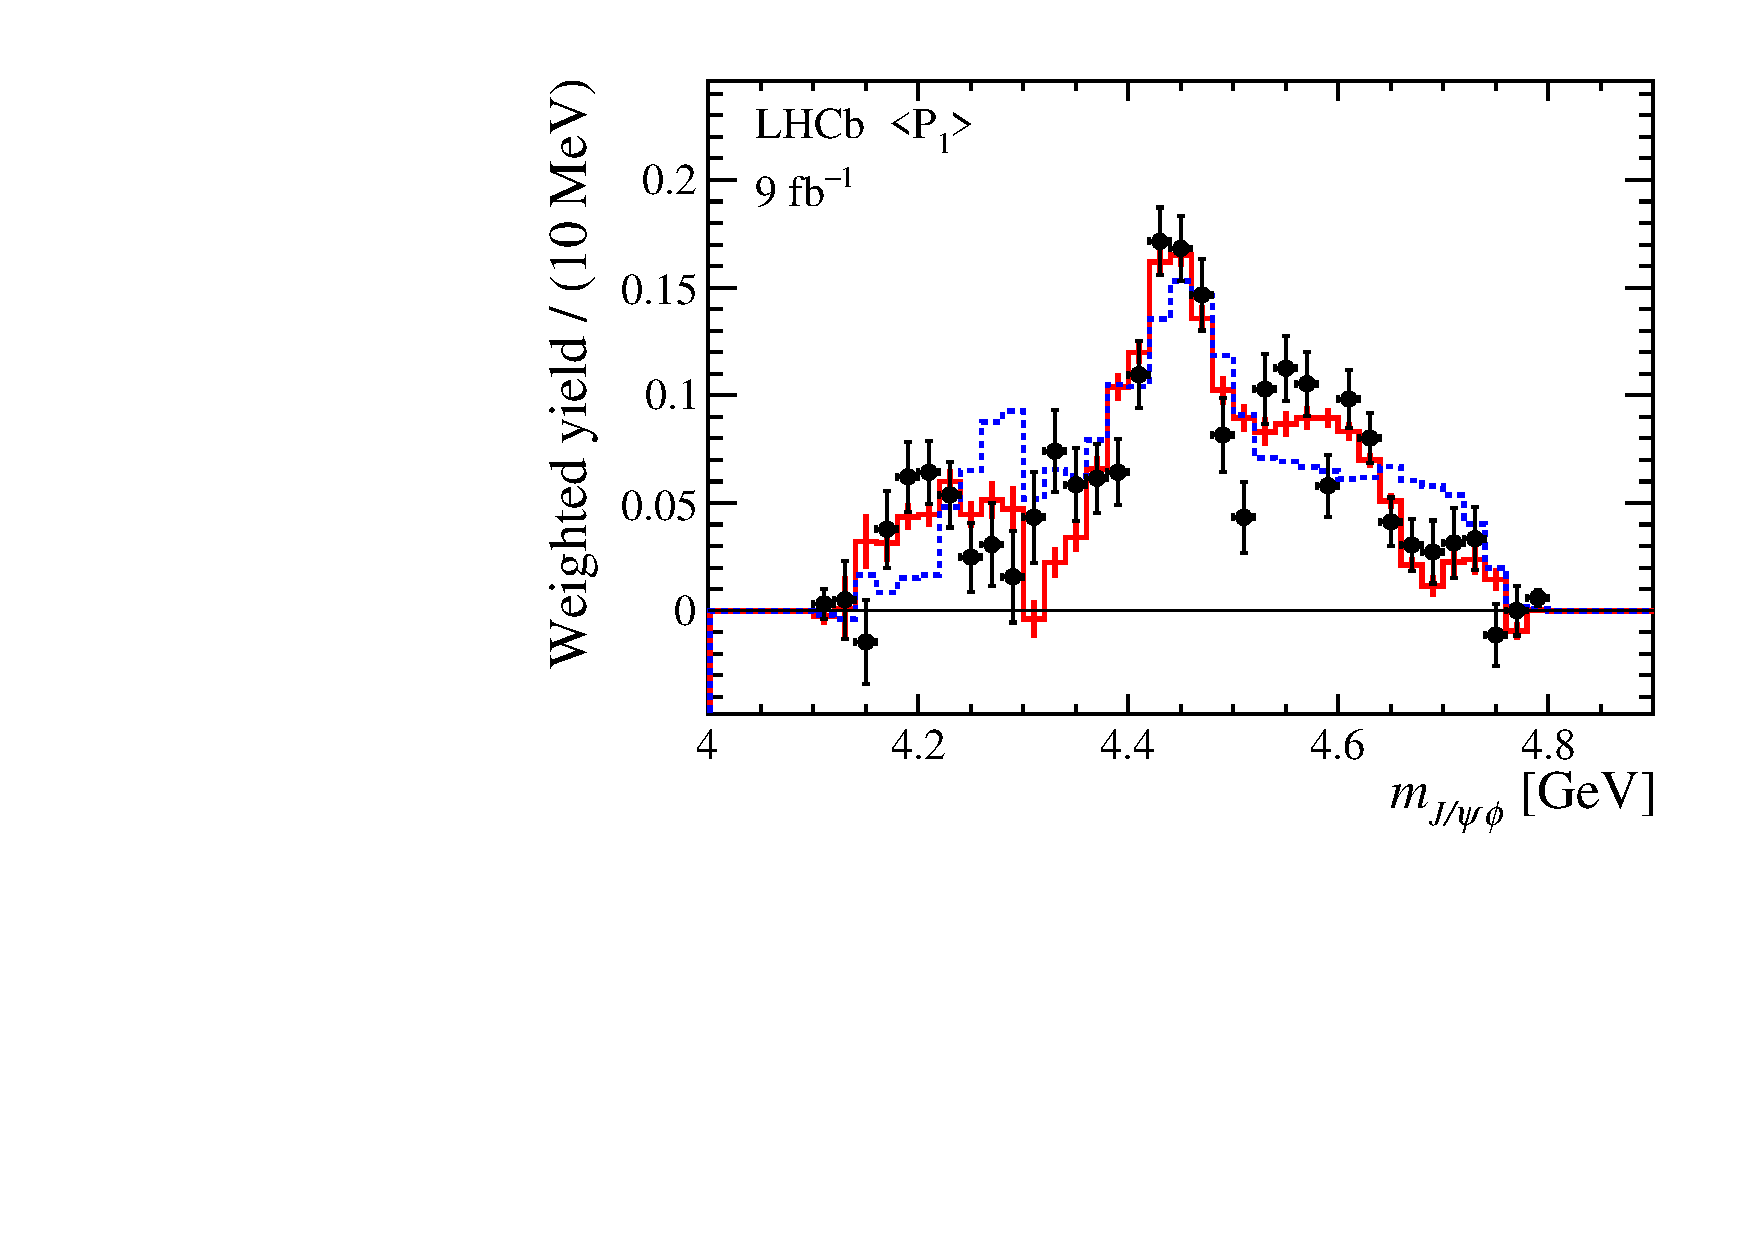
\includegraphics[width=0.33\textwidth]{Figures/03_Zcs/app_moments/shyphi1}%
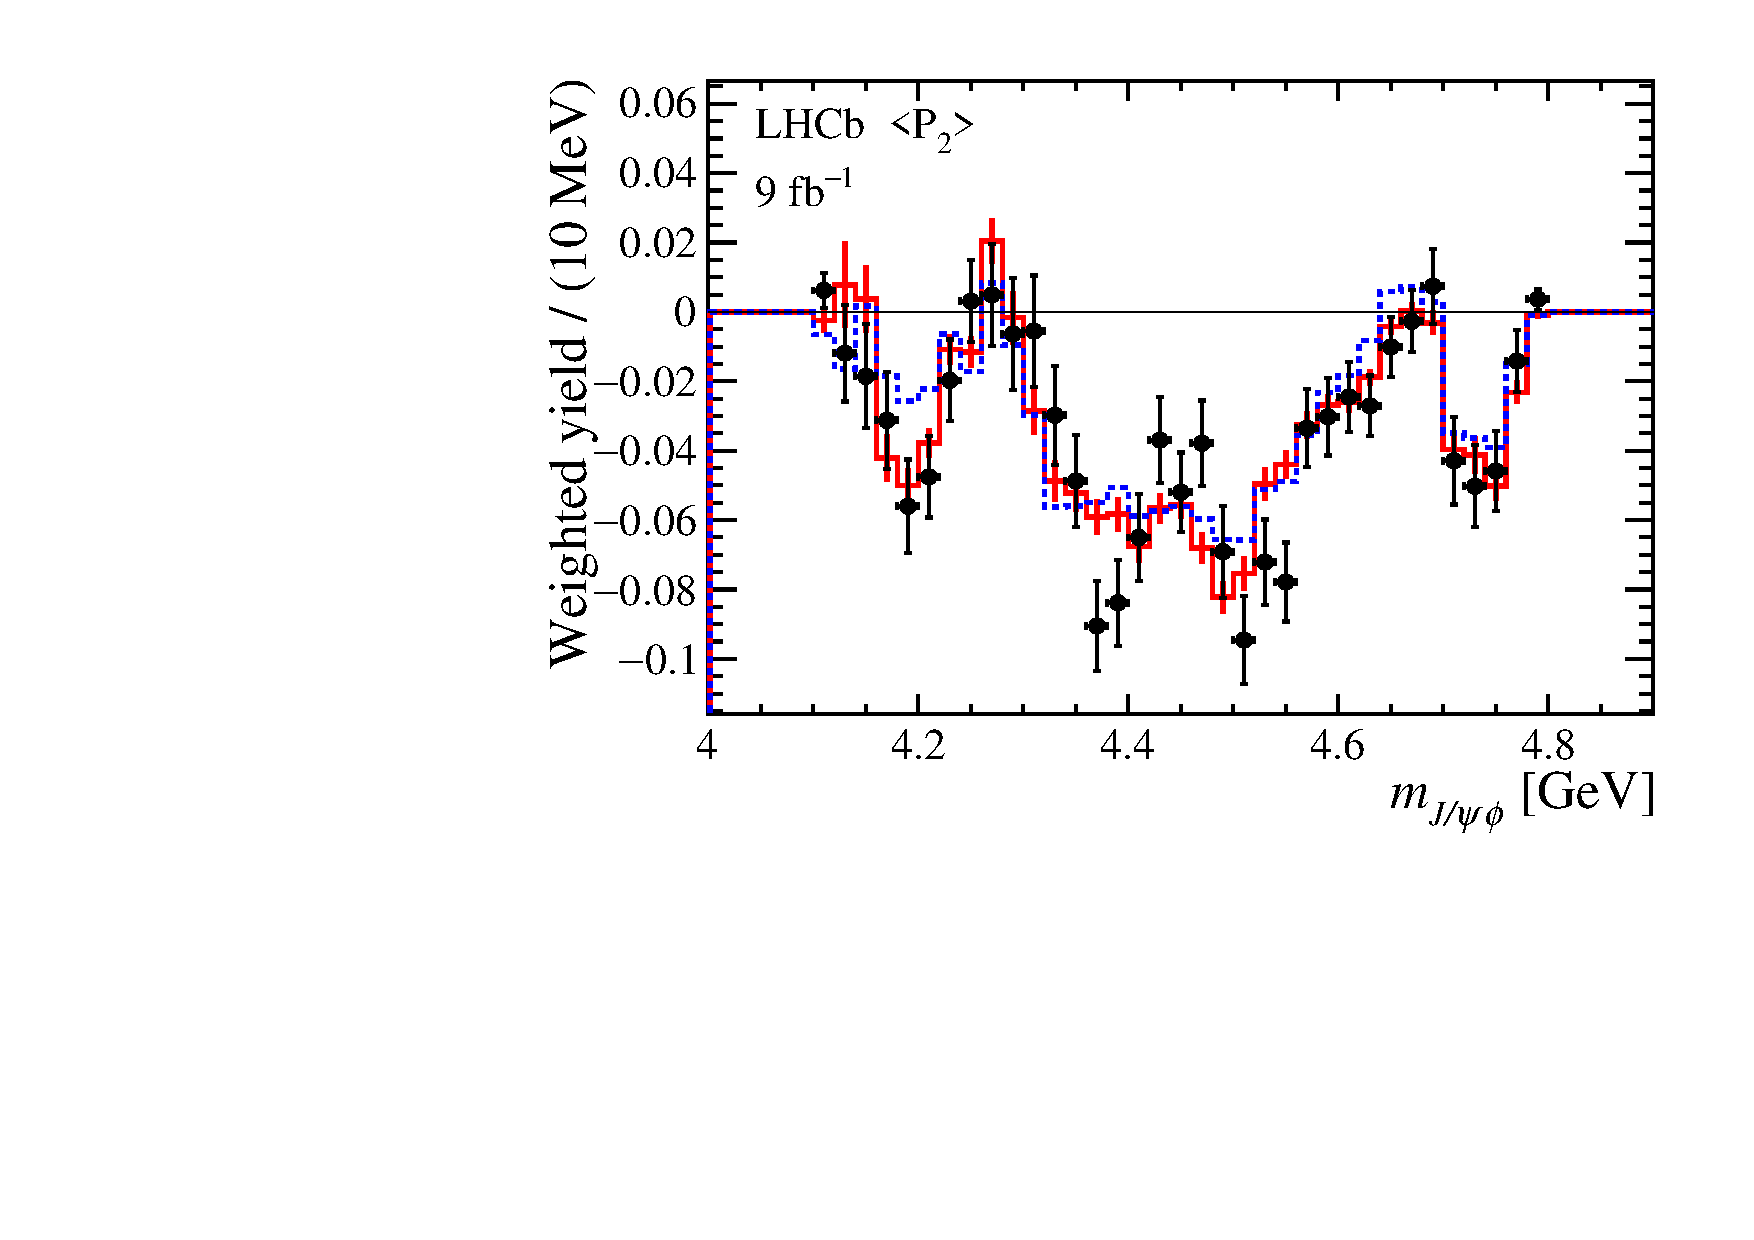
\includegraphics[width=0.33\textwidth]{Figures/03_Zcs/app_moments/shyphi2}
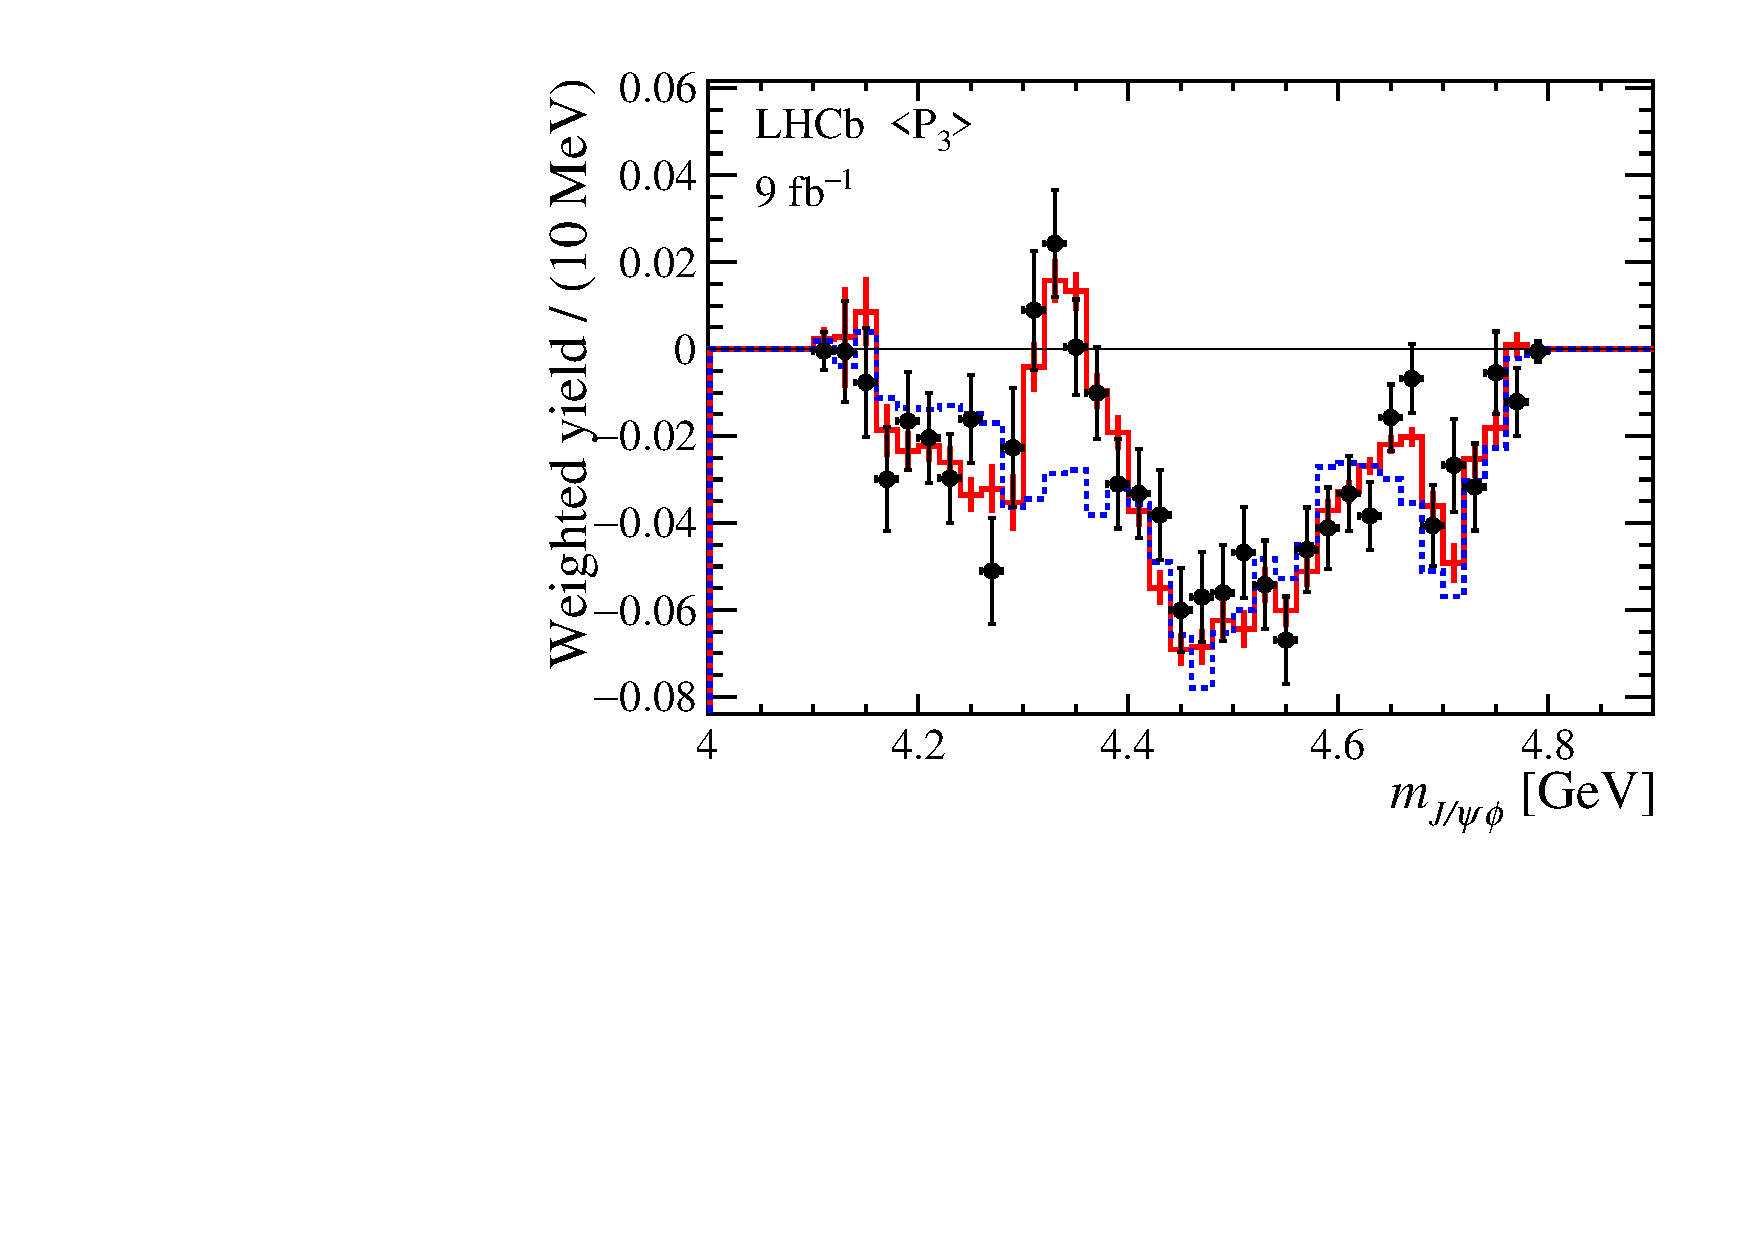
\includegraphics[width=0.33\textwidth]{Figures/03_Zcs/app_moments/shyphi3}%
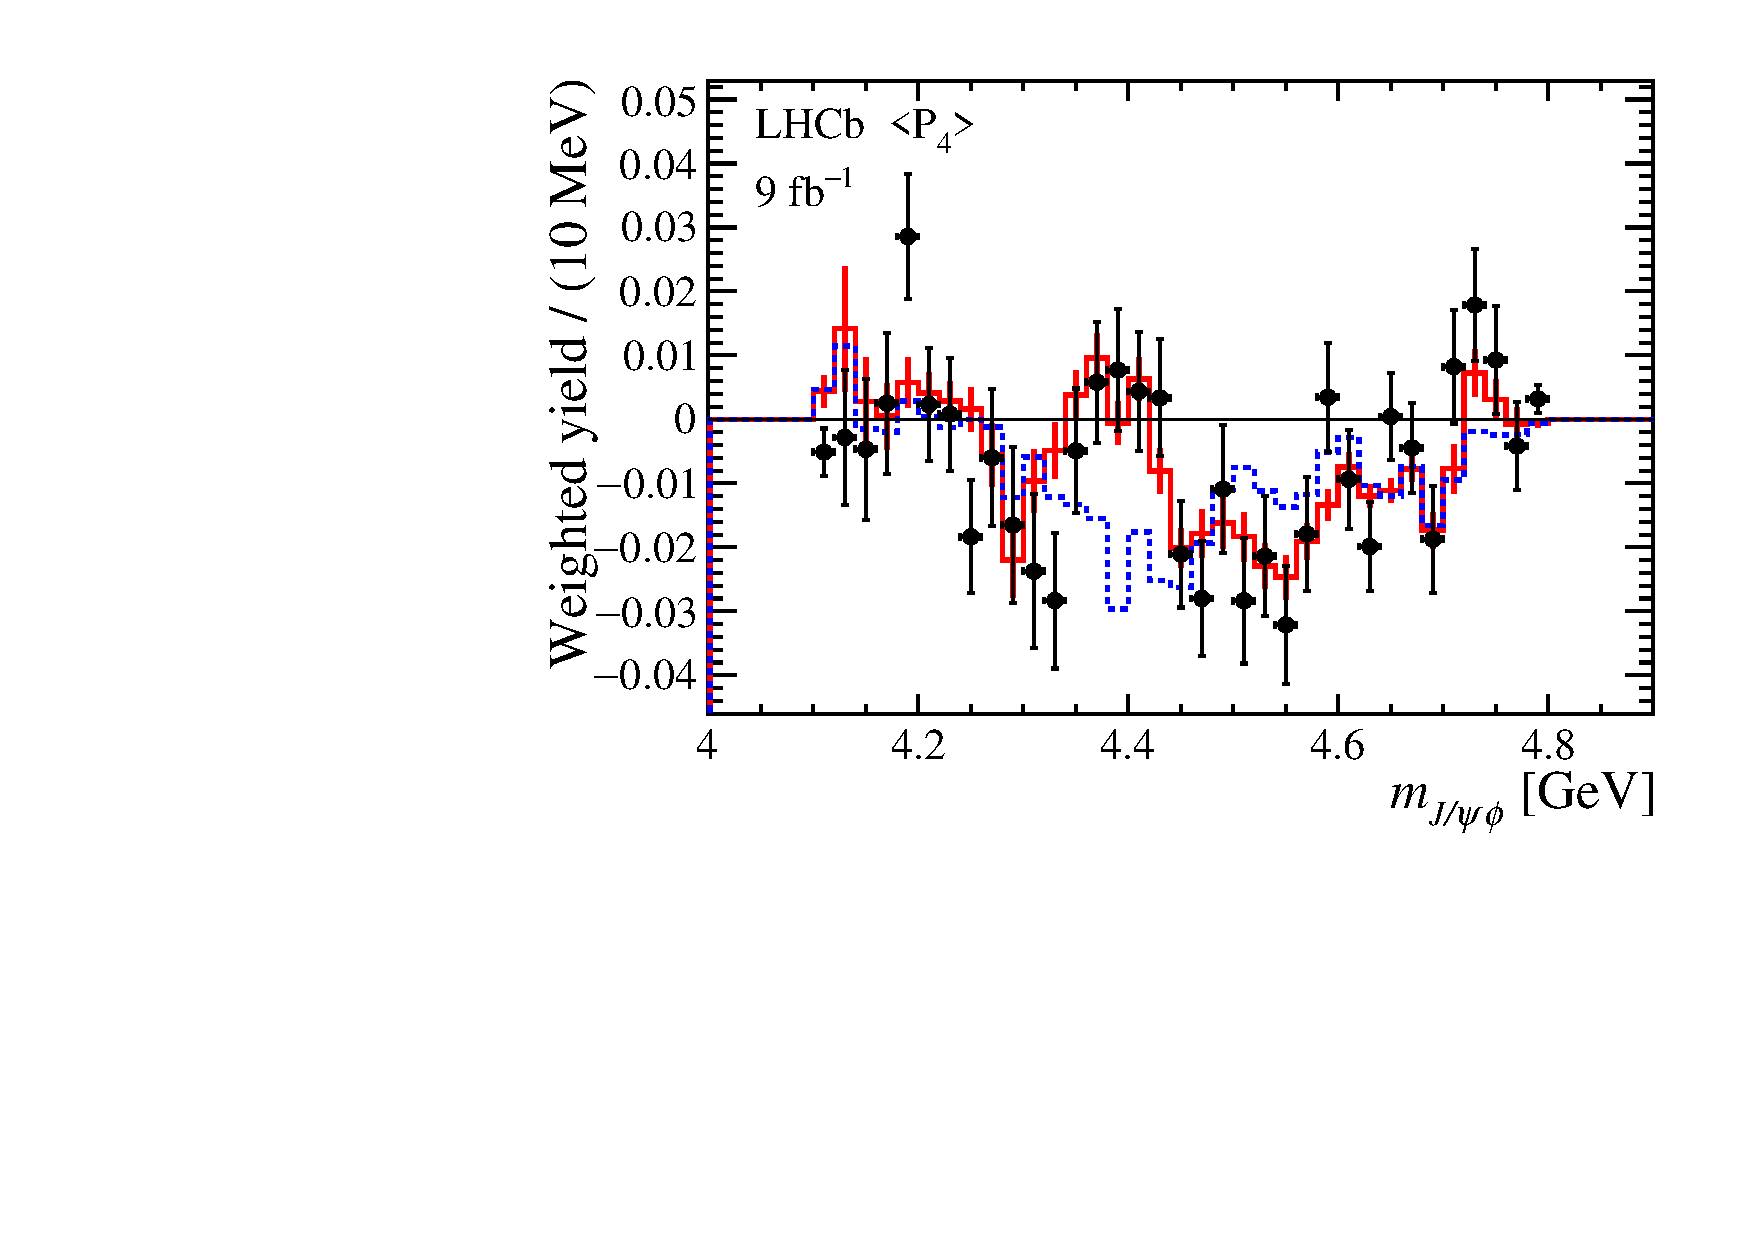
\includegraphics[width=0.33\textwidth]{Figures/03_Zcs/app_moments/shyphi4}%
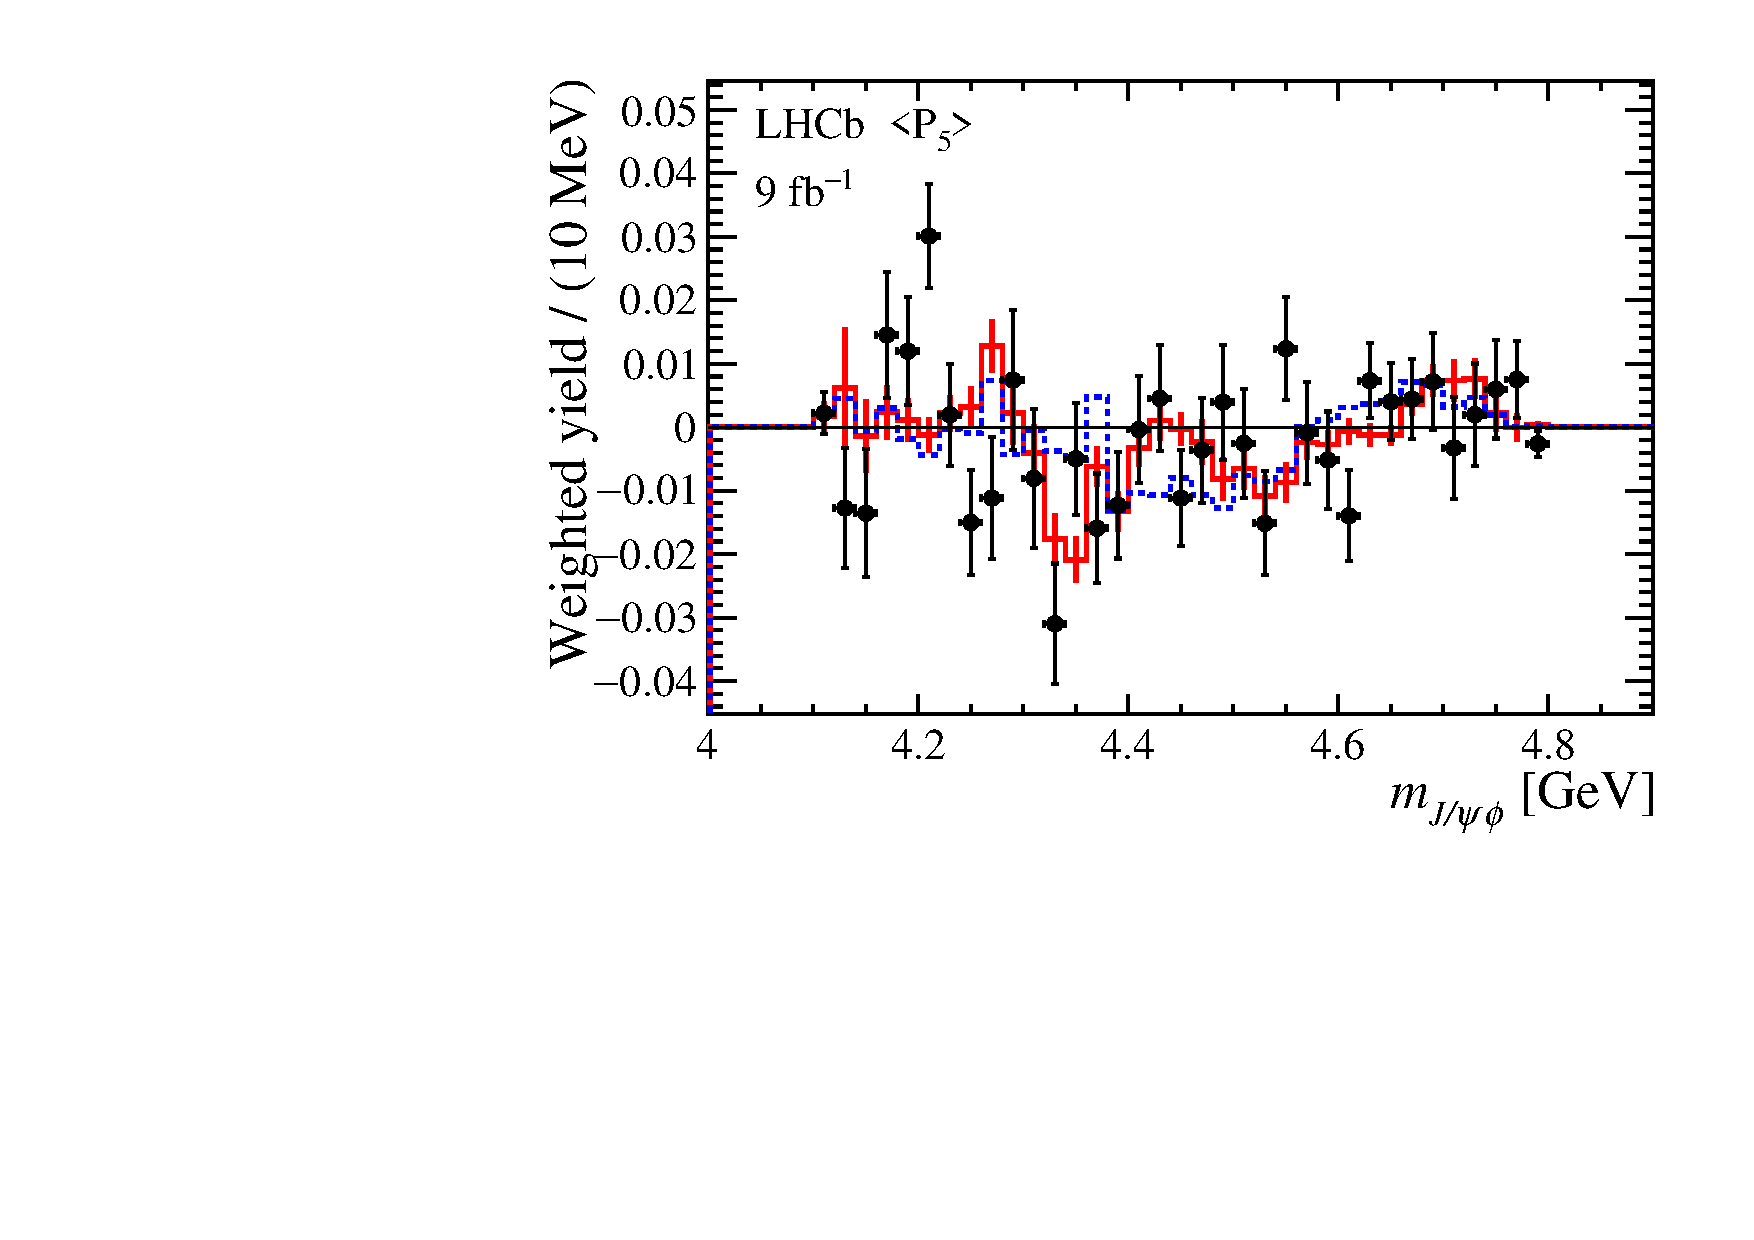
\includegraphics[width=0.33\textwidth]{Figures/03_Zcs/app_moments/shyphi5}
\caption{Angular moments of $\jpsi \phi$ helicity angle as a function of $\mjf$ compared between the background subtracted data, and PDFs from run1 model (blue dashed) and the nominal model (red solid). The $\chi^2/$nbin for the fit of nominal model (run1 model) are 83(136)/69, 59(117)/35, 48(89)/35, 33(89)/35, 42(81)/35, 55(65)/35 for order from 0 to 5, respectively.  }
\label{mom5phi}
\end{figure}



\begin{figure}[!htbp]
\centering
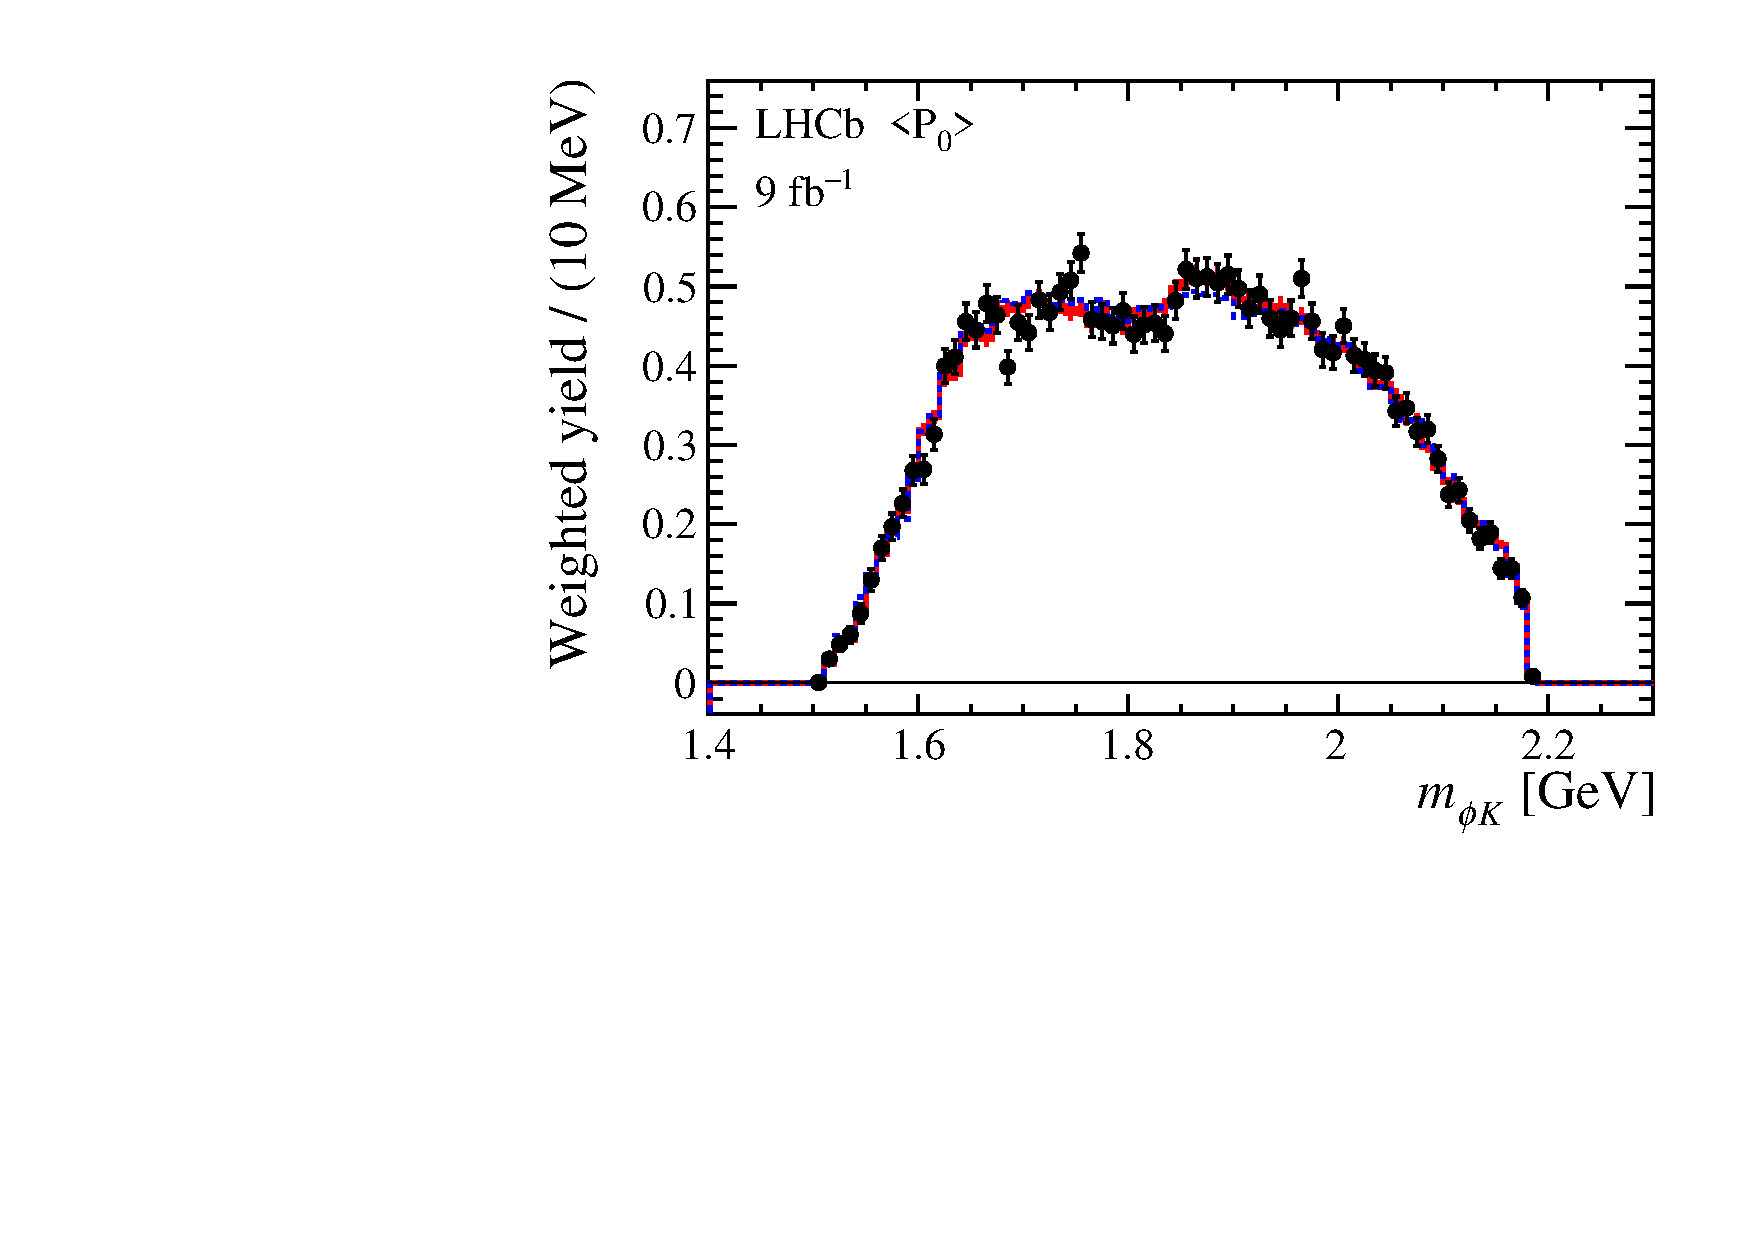
\includegraphics[width=0.33\textwidth]{Figures/03_Zcs/app_moments/shykst0}%
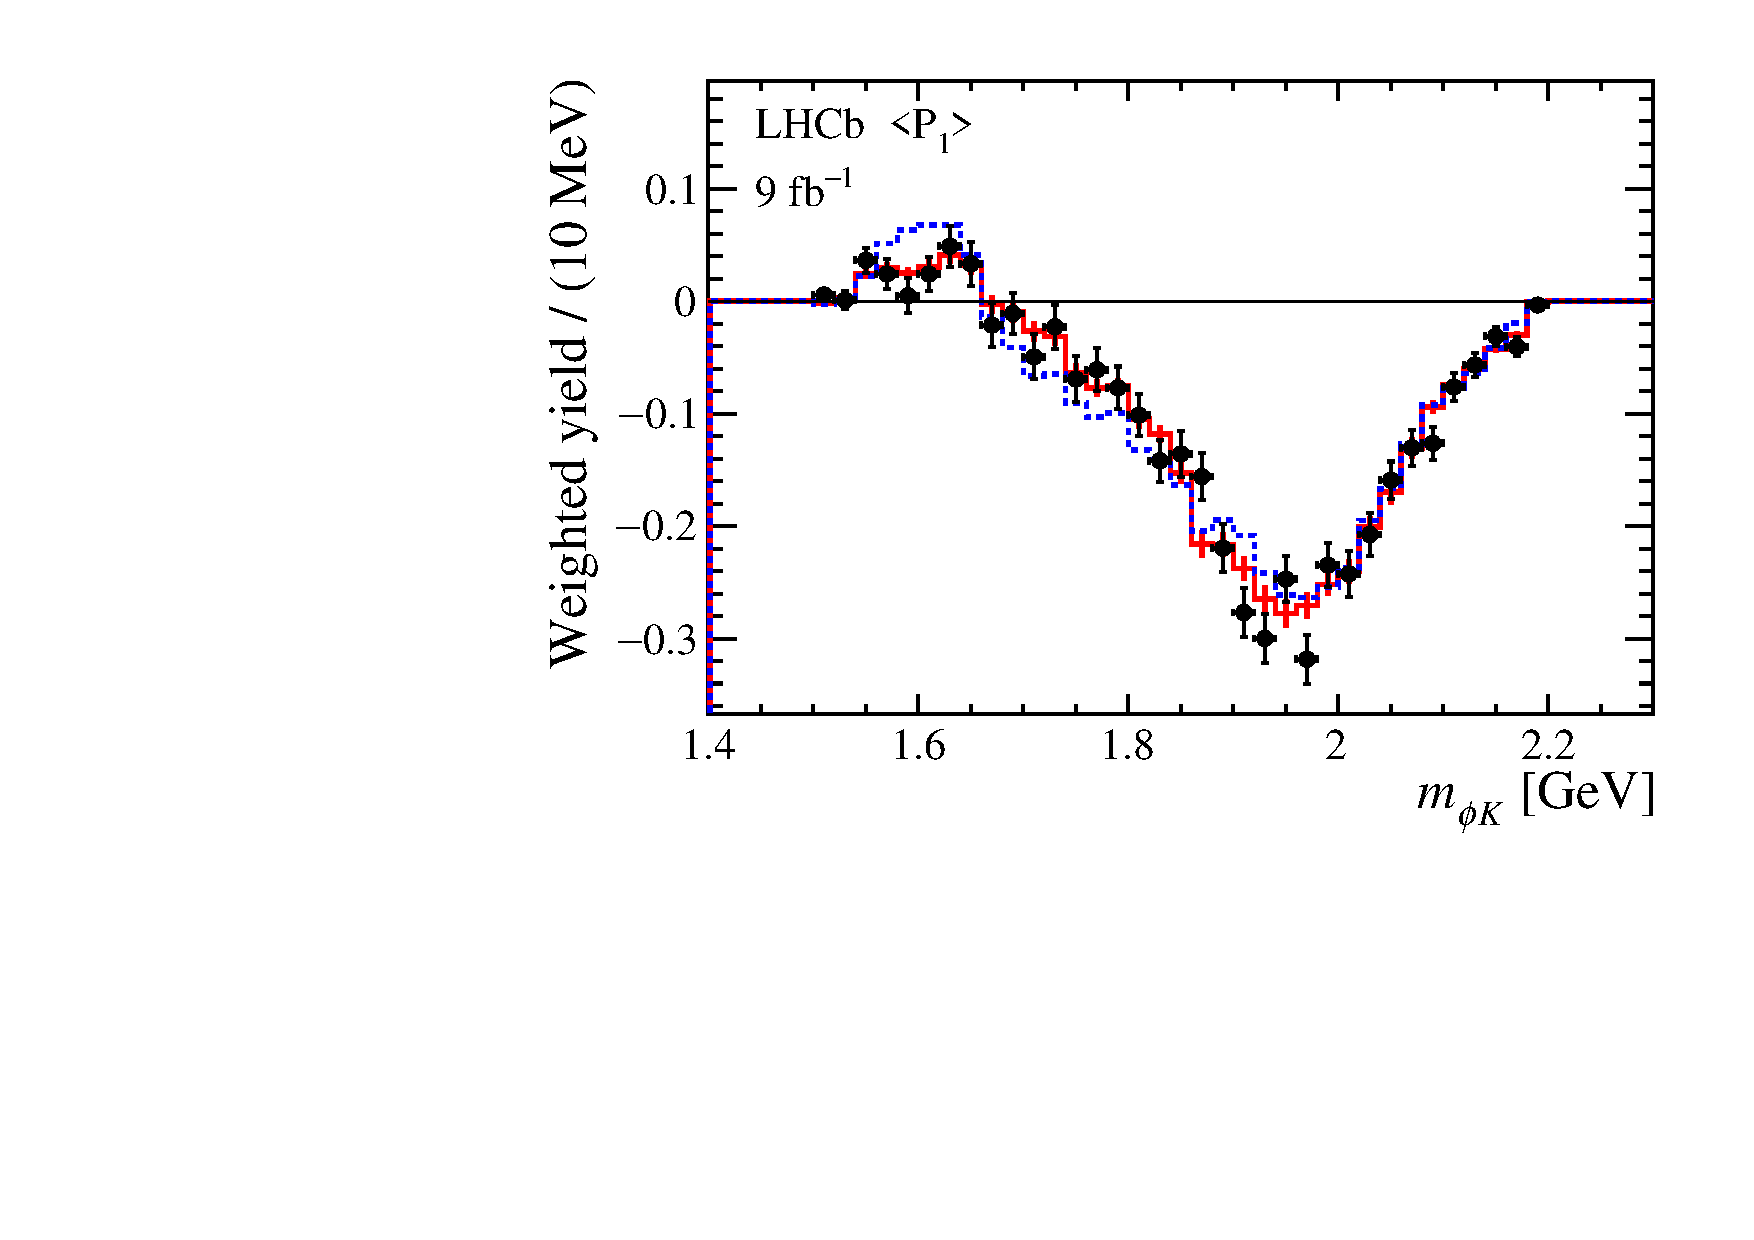
\includegraphics[width=0.33\textwidth]{Figures/03_Zcs/app_moments/shykst1}%
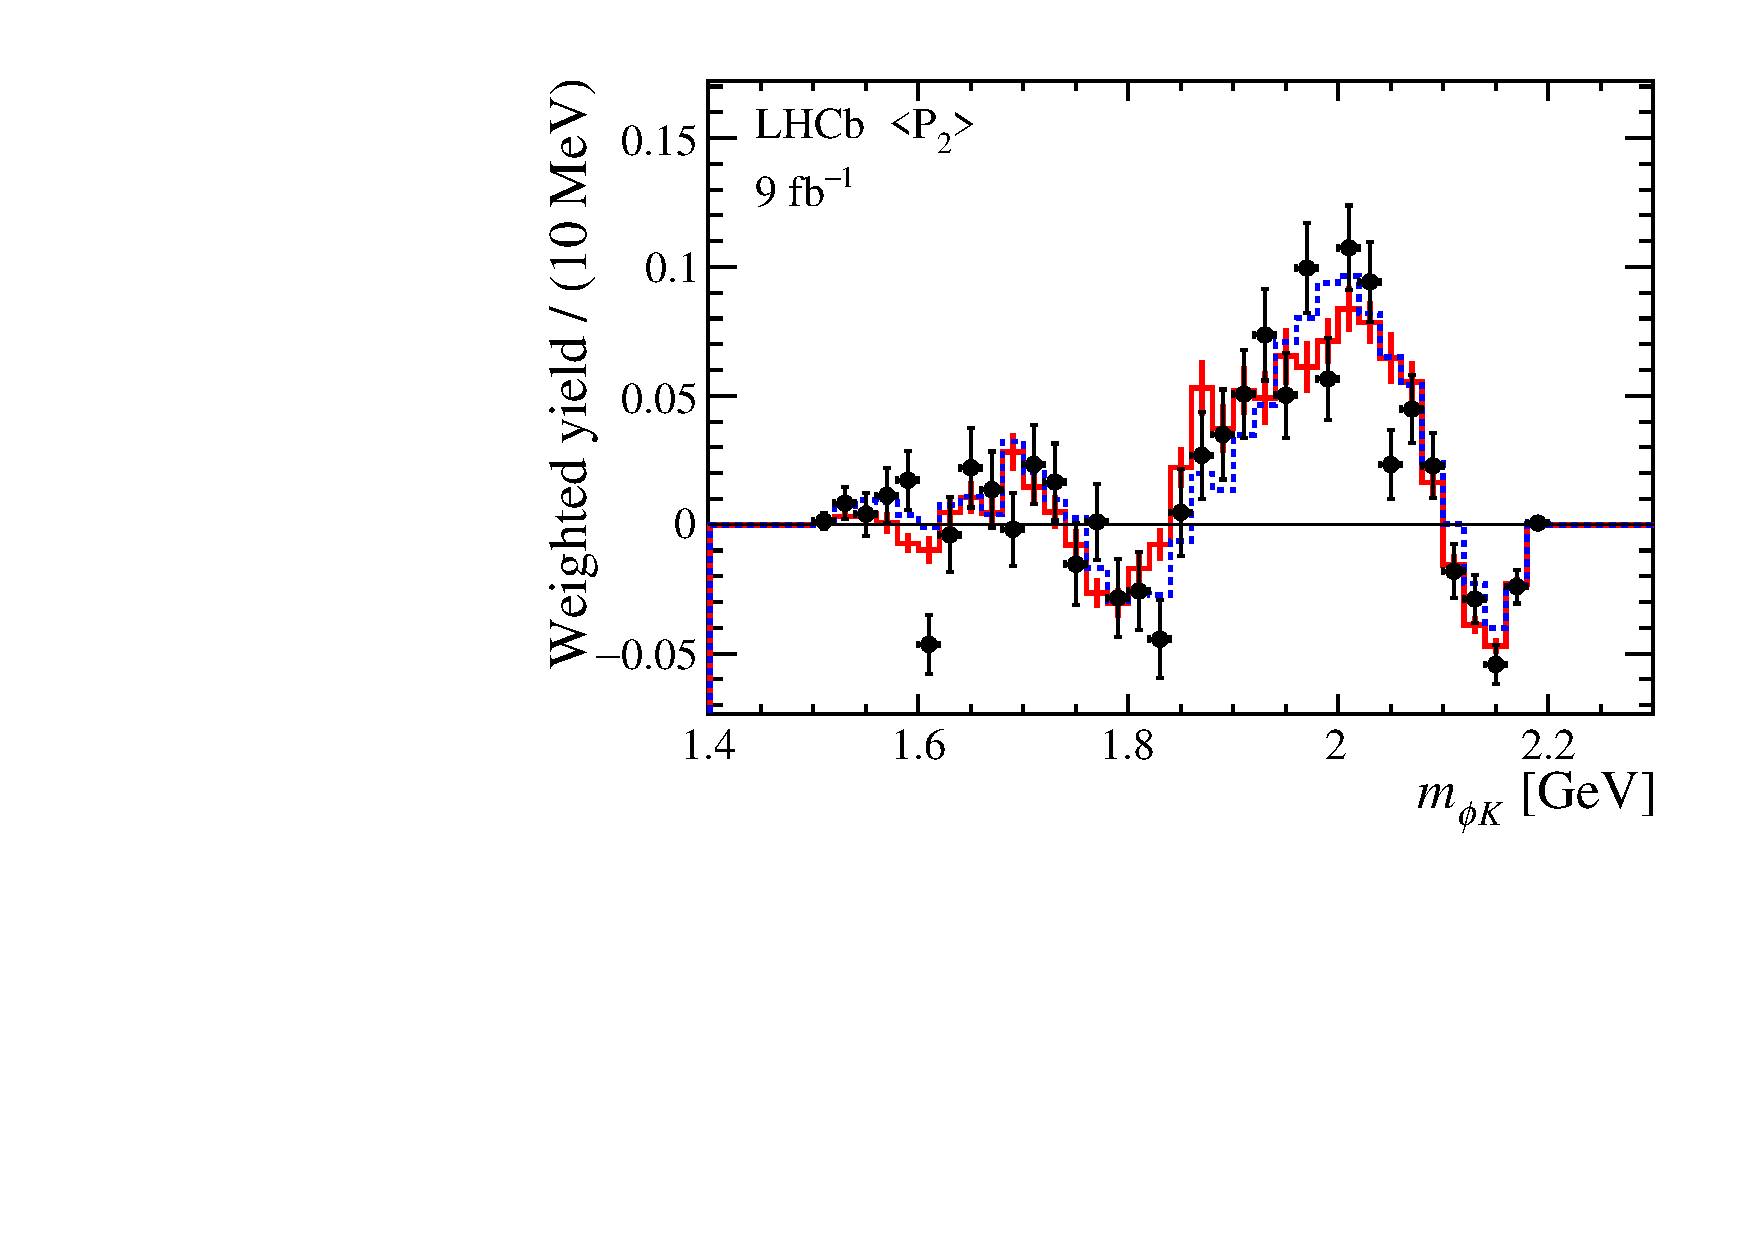
\includegraphics[width=0.33\textwidth]{Figures/03_Zcs/app_moments/shykst2}
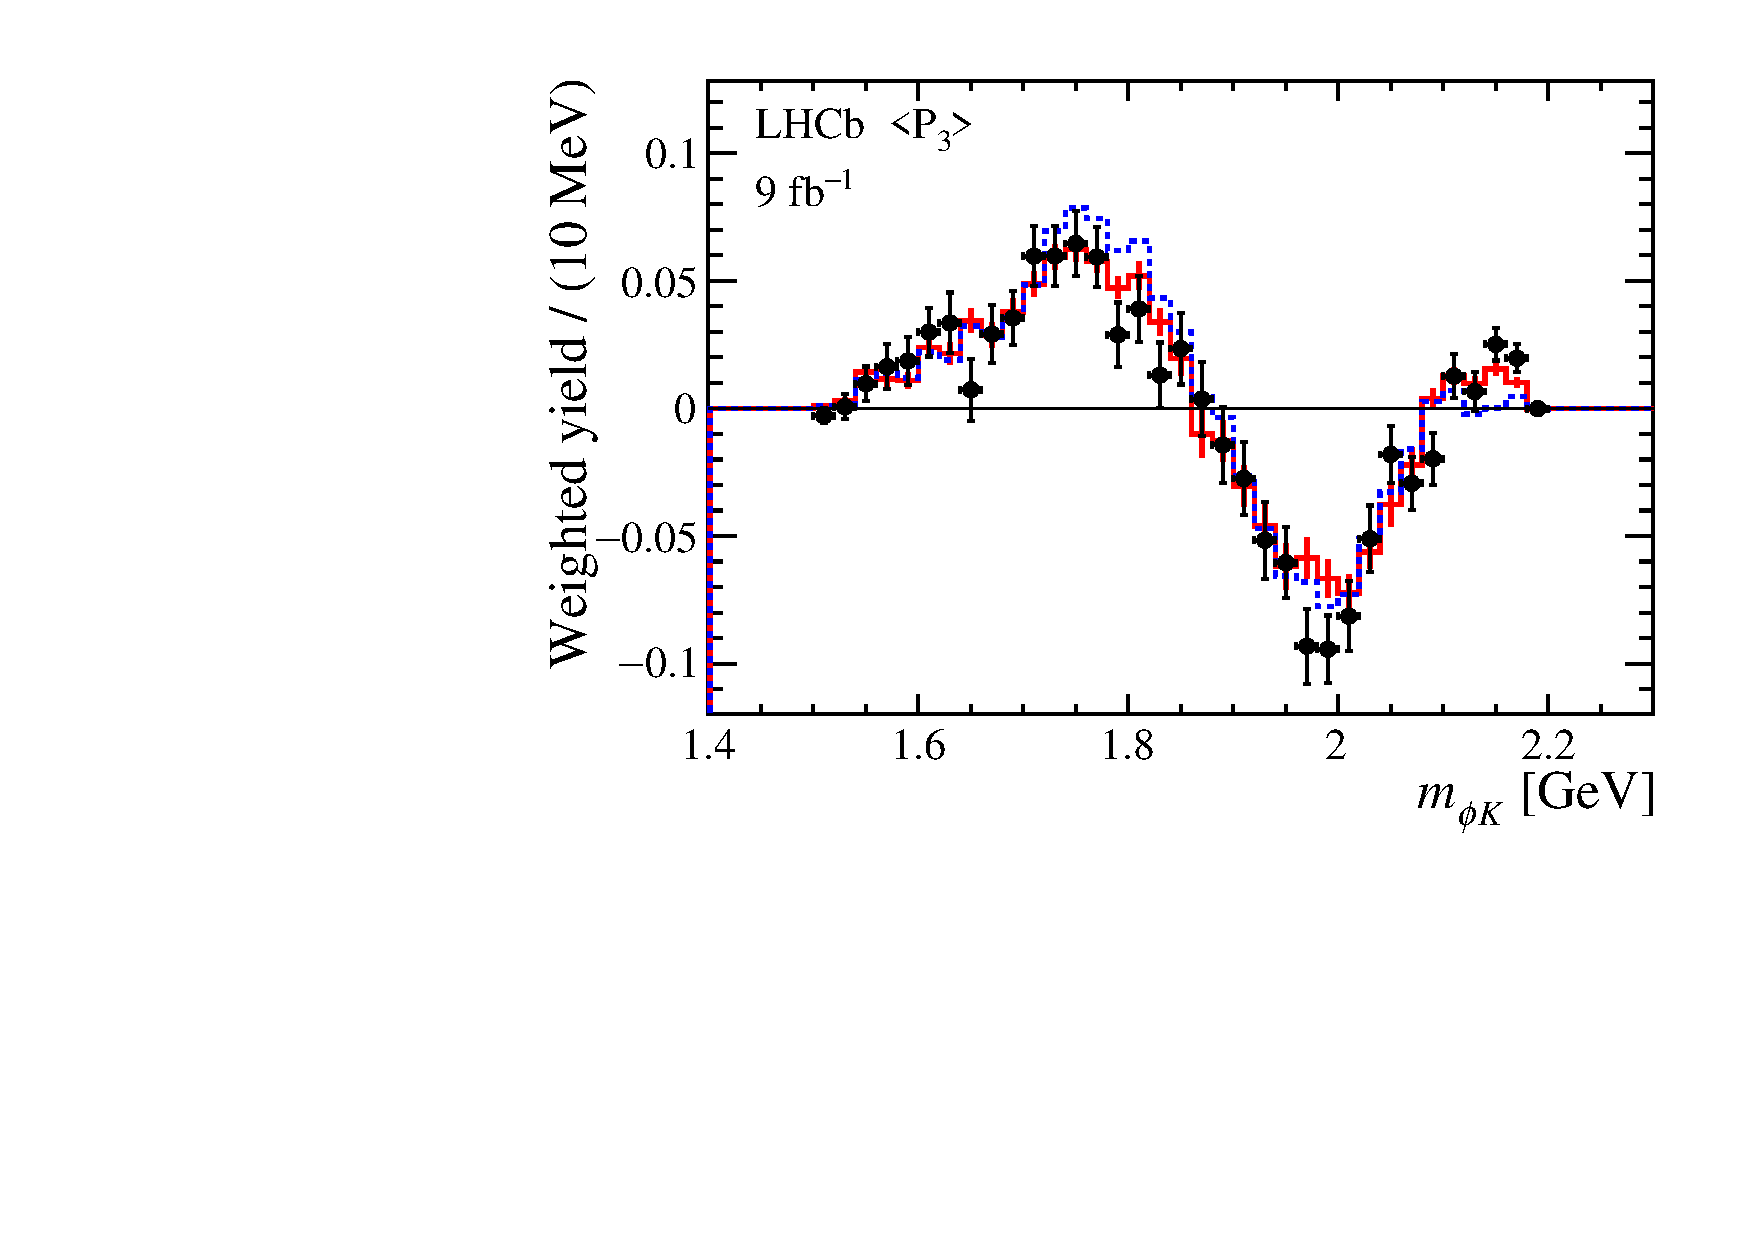
\includegraphics[width=0.33\textwidth]{Figures/03_Zcs/app_moments/shykst3}%
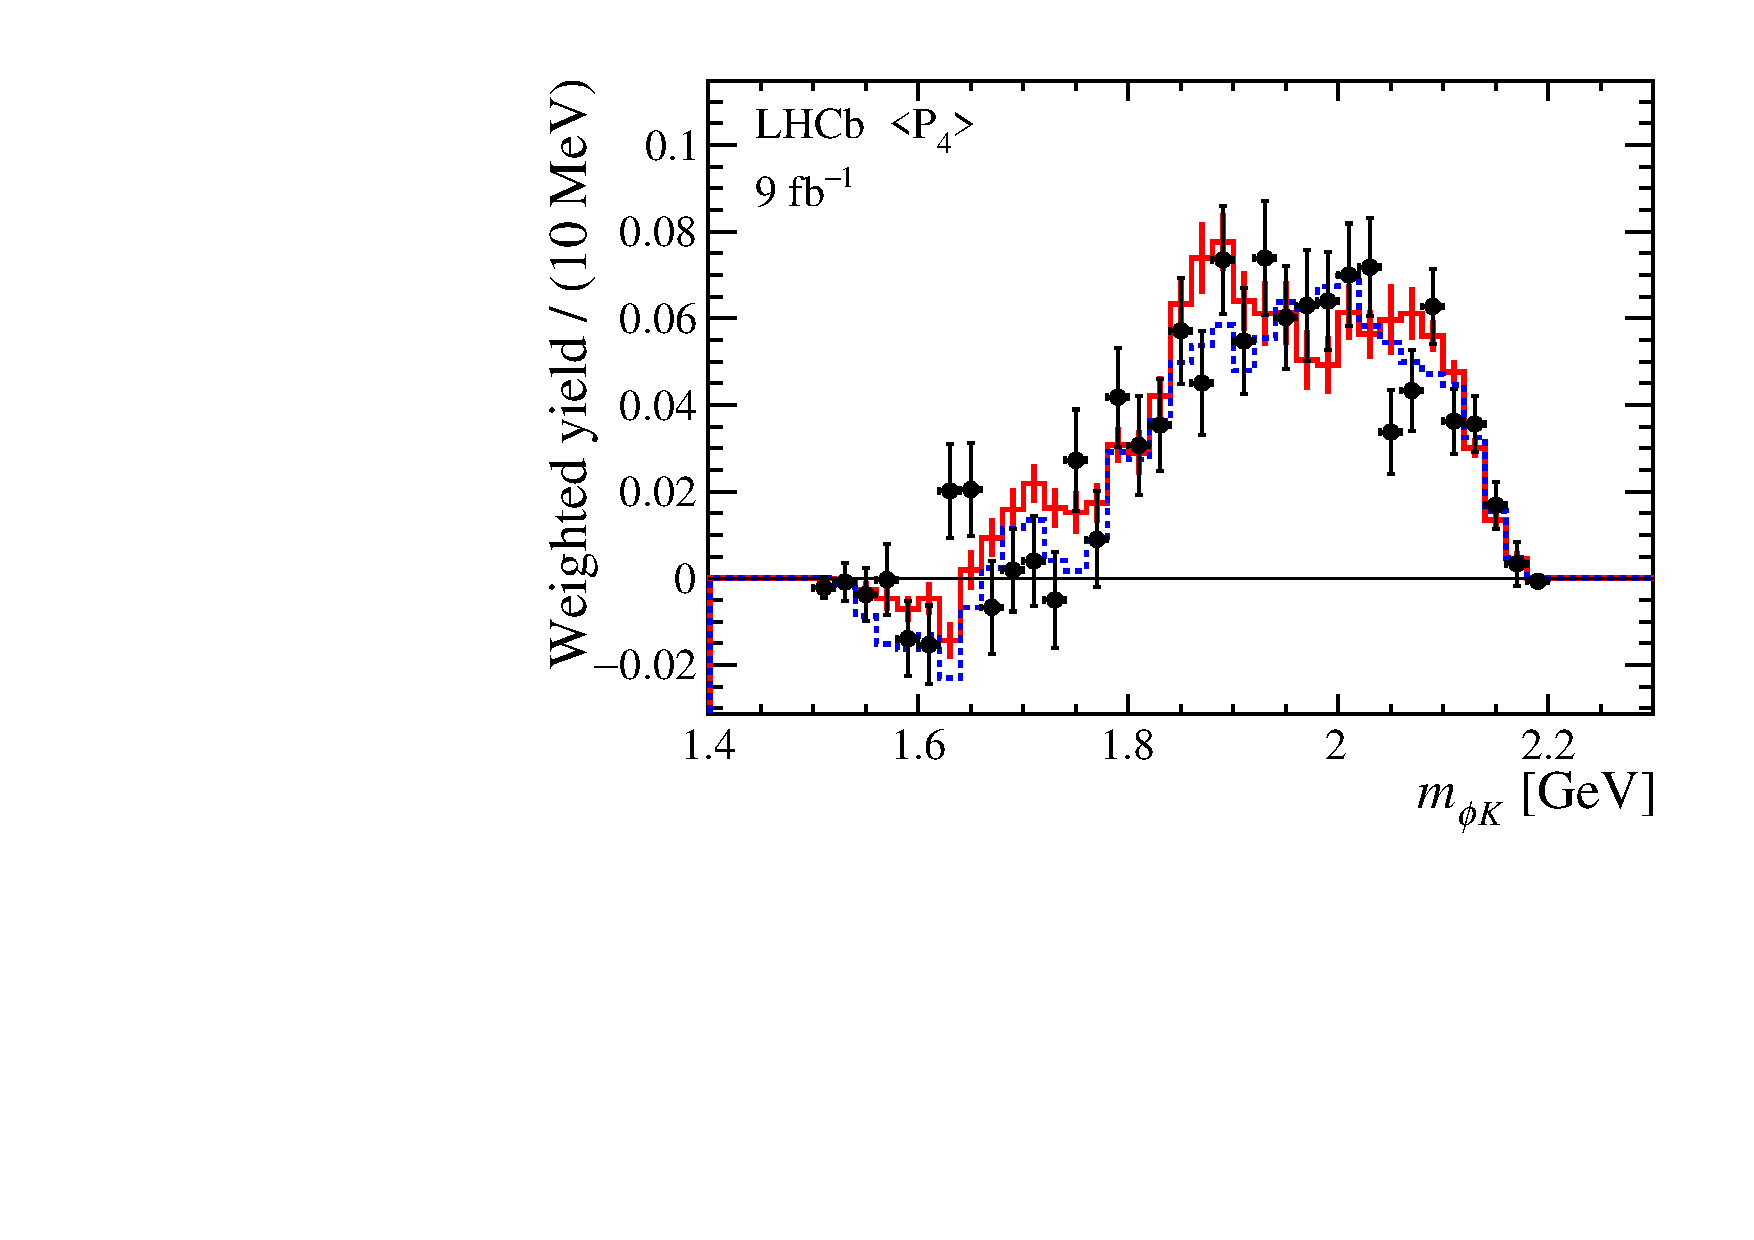
\includegraphics[width=0.33\textwidth]{Figures/03_Zcs/app_moments/shykst4}%
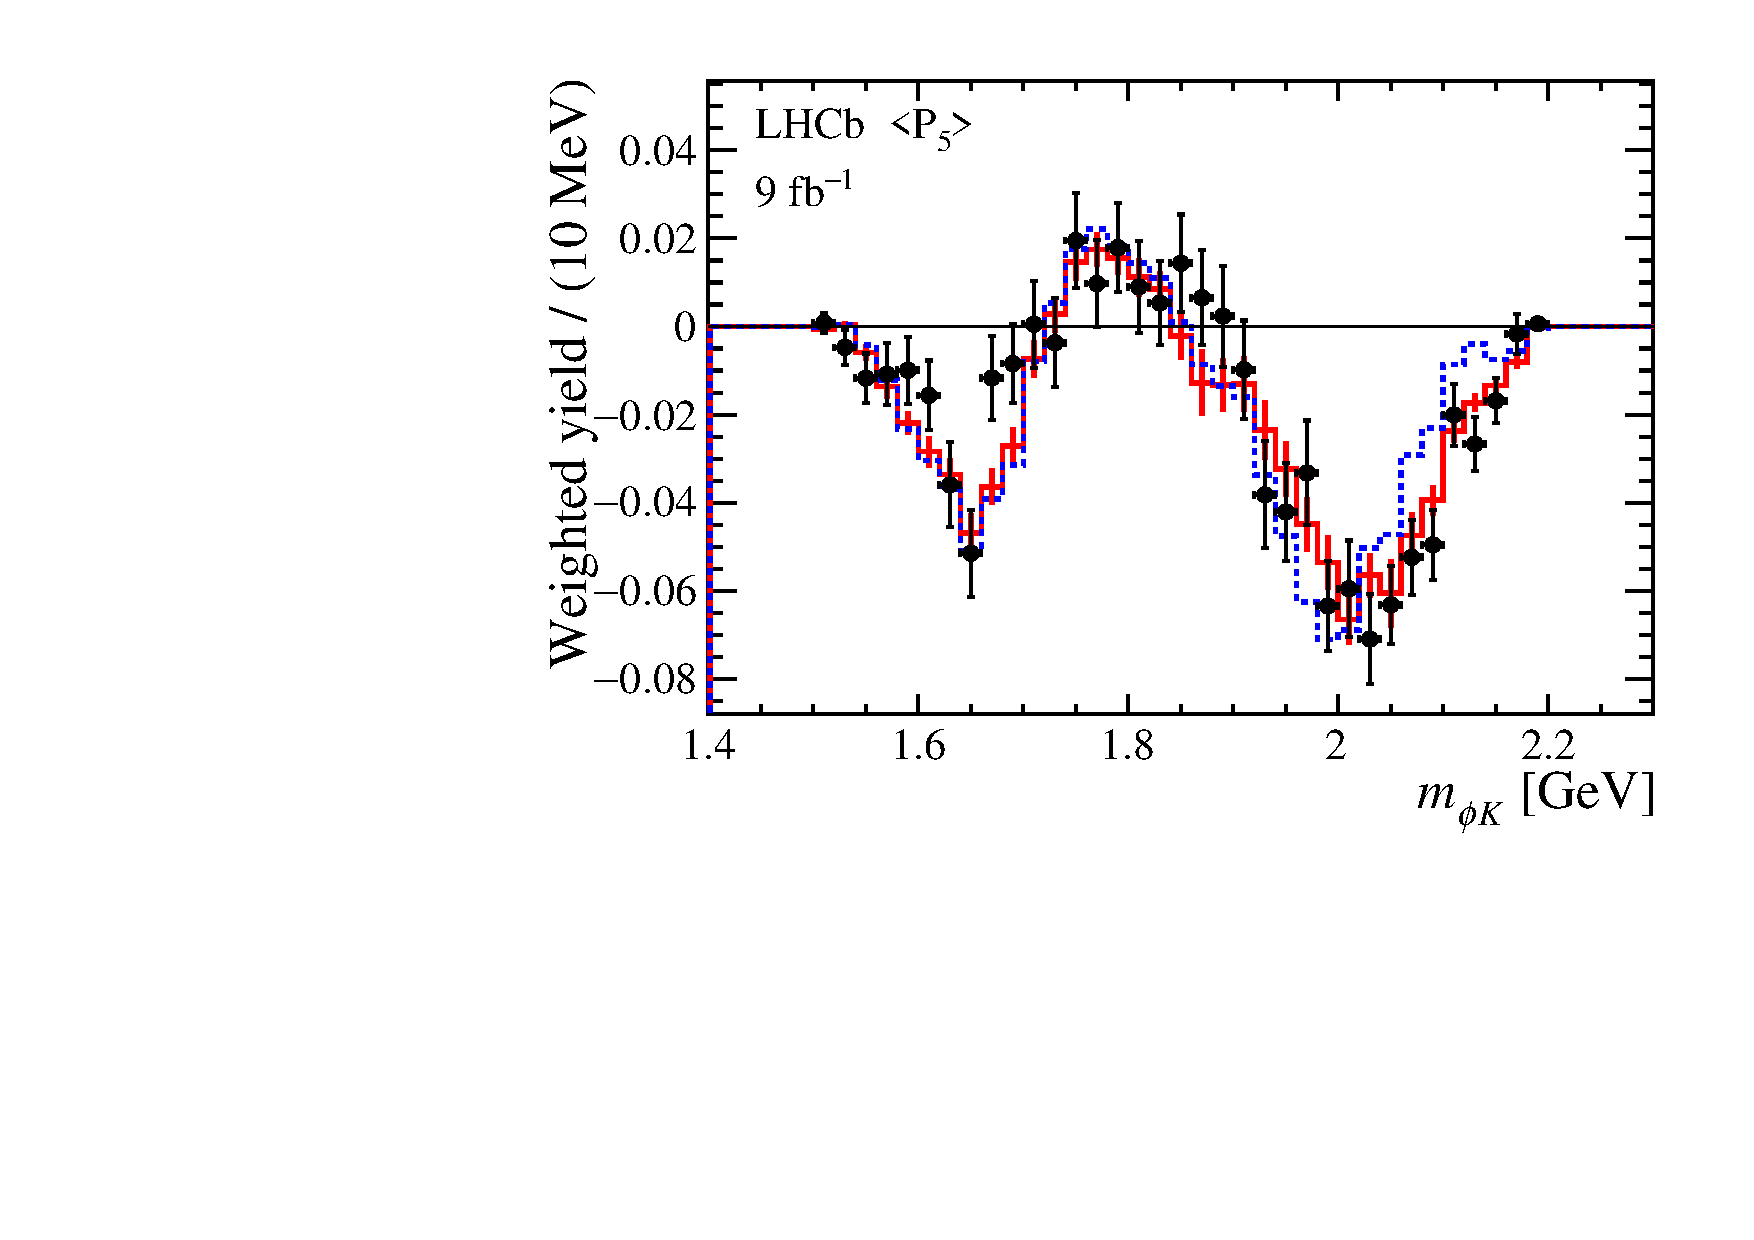
\includegraphics[width=0.33\textwidth]{Figures/03_Zcs/app_moments/shykst5}
\caption{Signal angular moments of $\phi K$ helicity angle as a function of $\mfk$ compared between the background subtracted data, and PDFs from run1 model (blue dashed) and the nominal model (red solid). The $\chi^2/$nbin for the fit of nominal model (run1 model) are 66(79)/69, 37(86)/35, 49(48)/35, 35(59)/35, 46(44)/35, 36(74)/35 for order from 0 to 5, respectively.}
\label{mom5kst}
\end{figure}

\begin{figure}[!htbp]
\centering
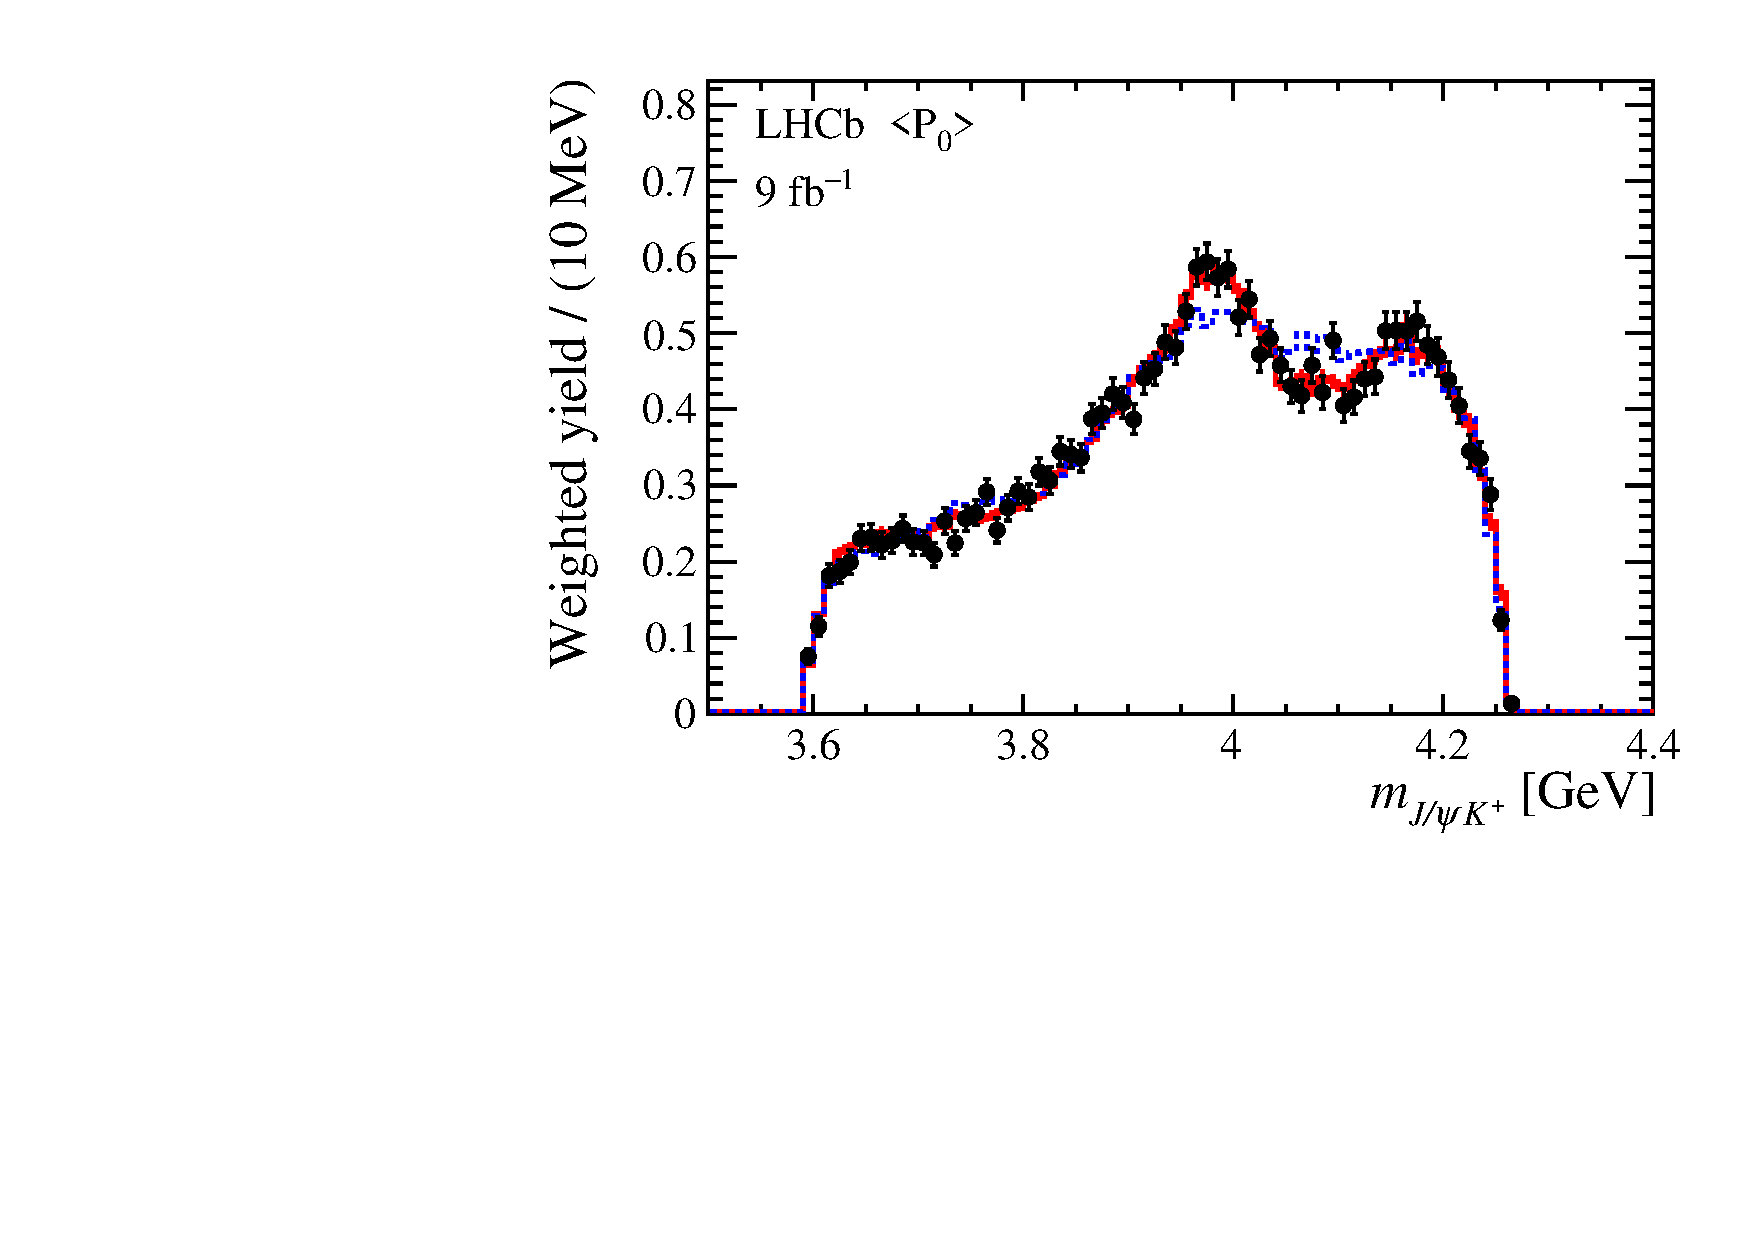
\includegraphics[width=0.33\textwidth]{Figures/03_Zcs/app_moments/shy1z0}%
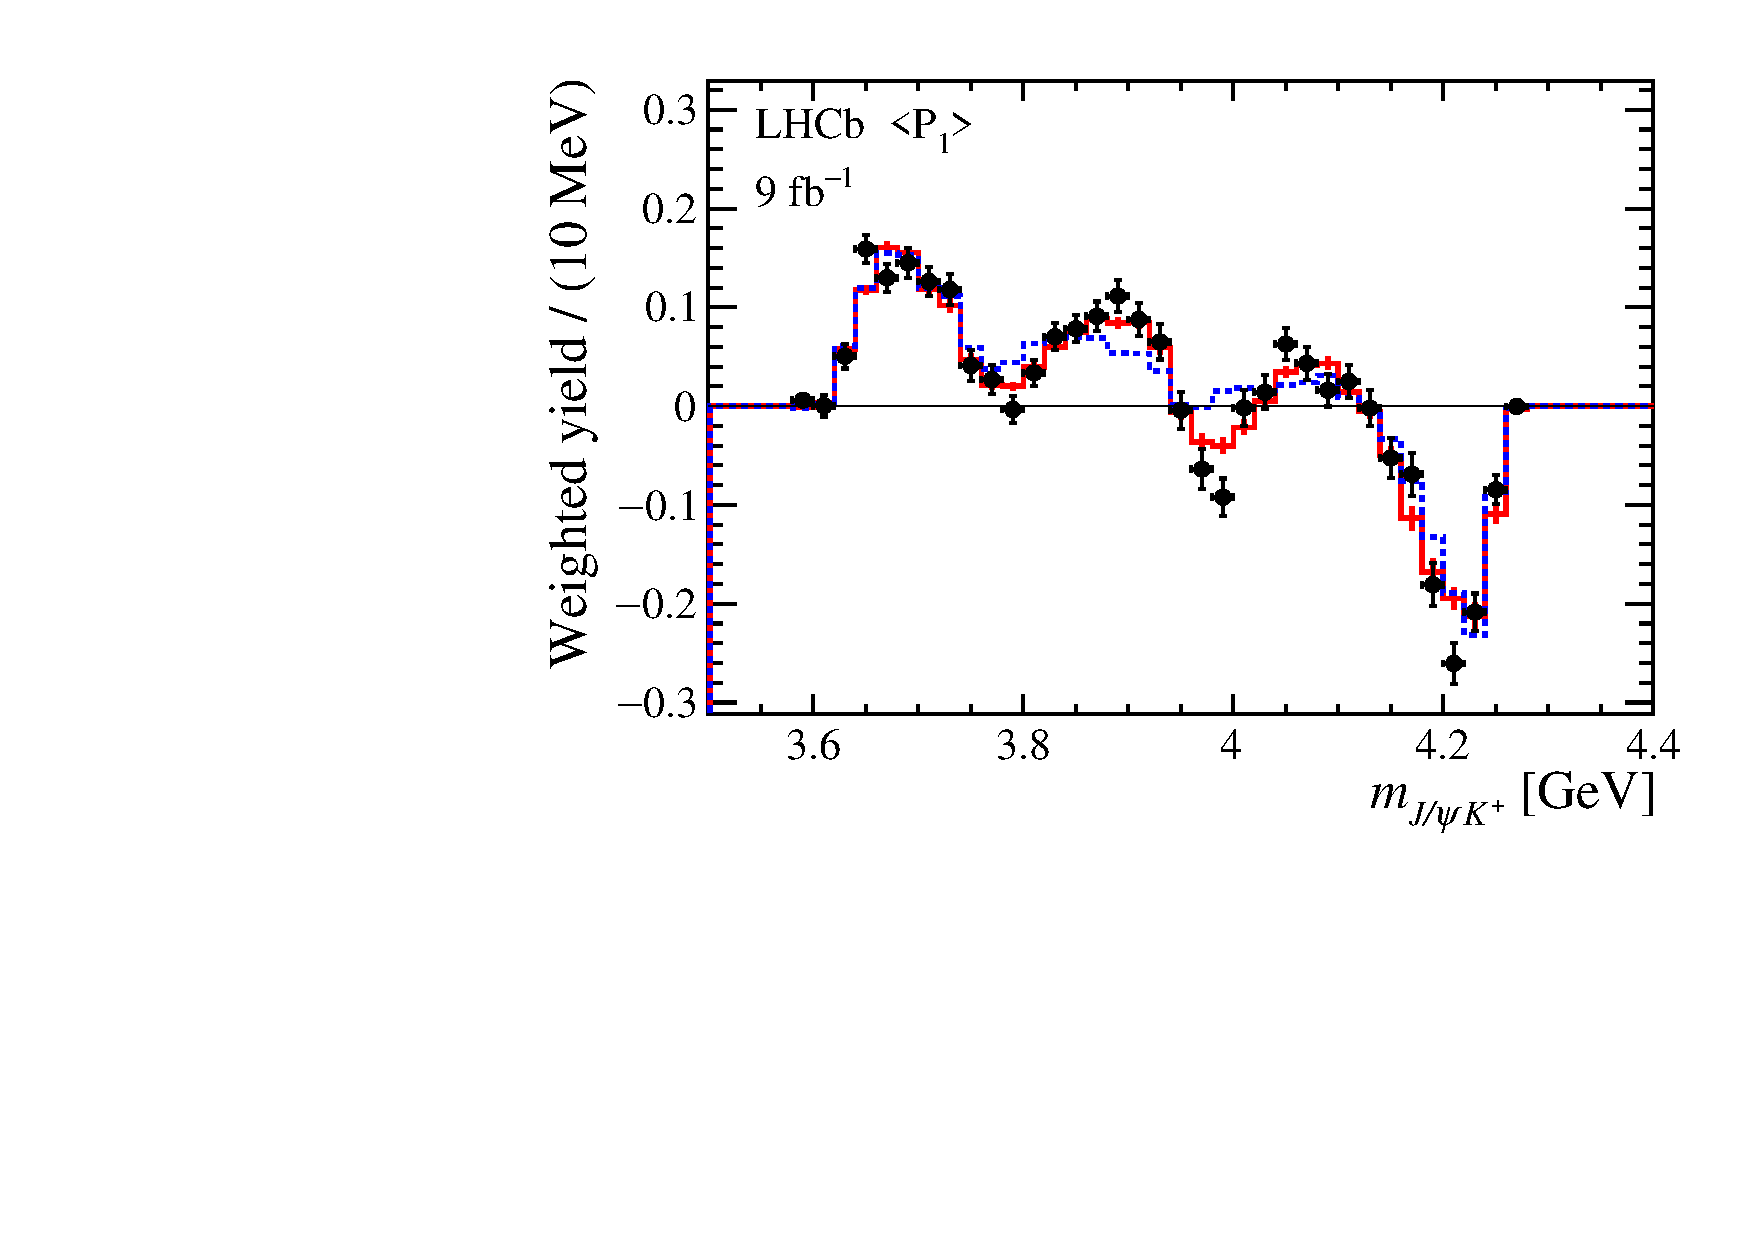
\includegraphics[width=0.33\textwidth]{Figures/03_Zcs/app_moments/shy1z1}%
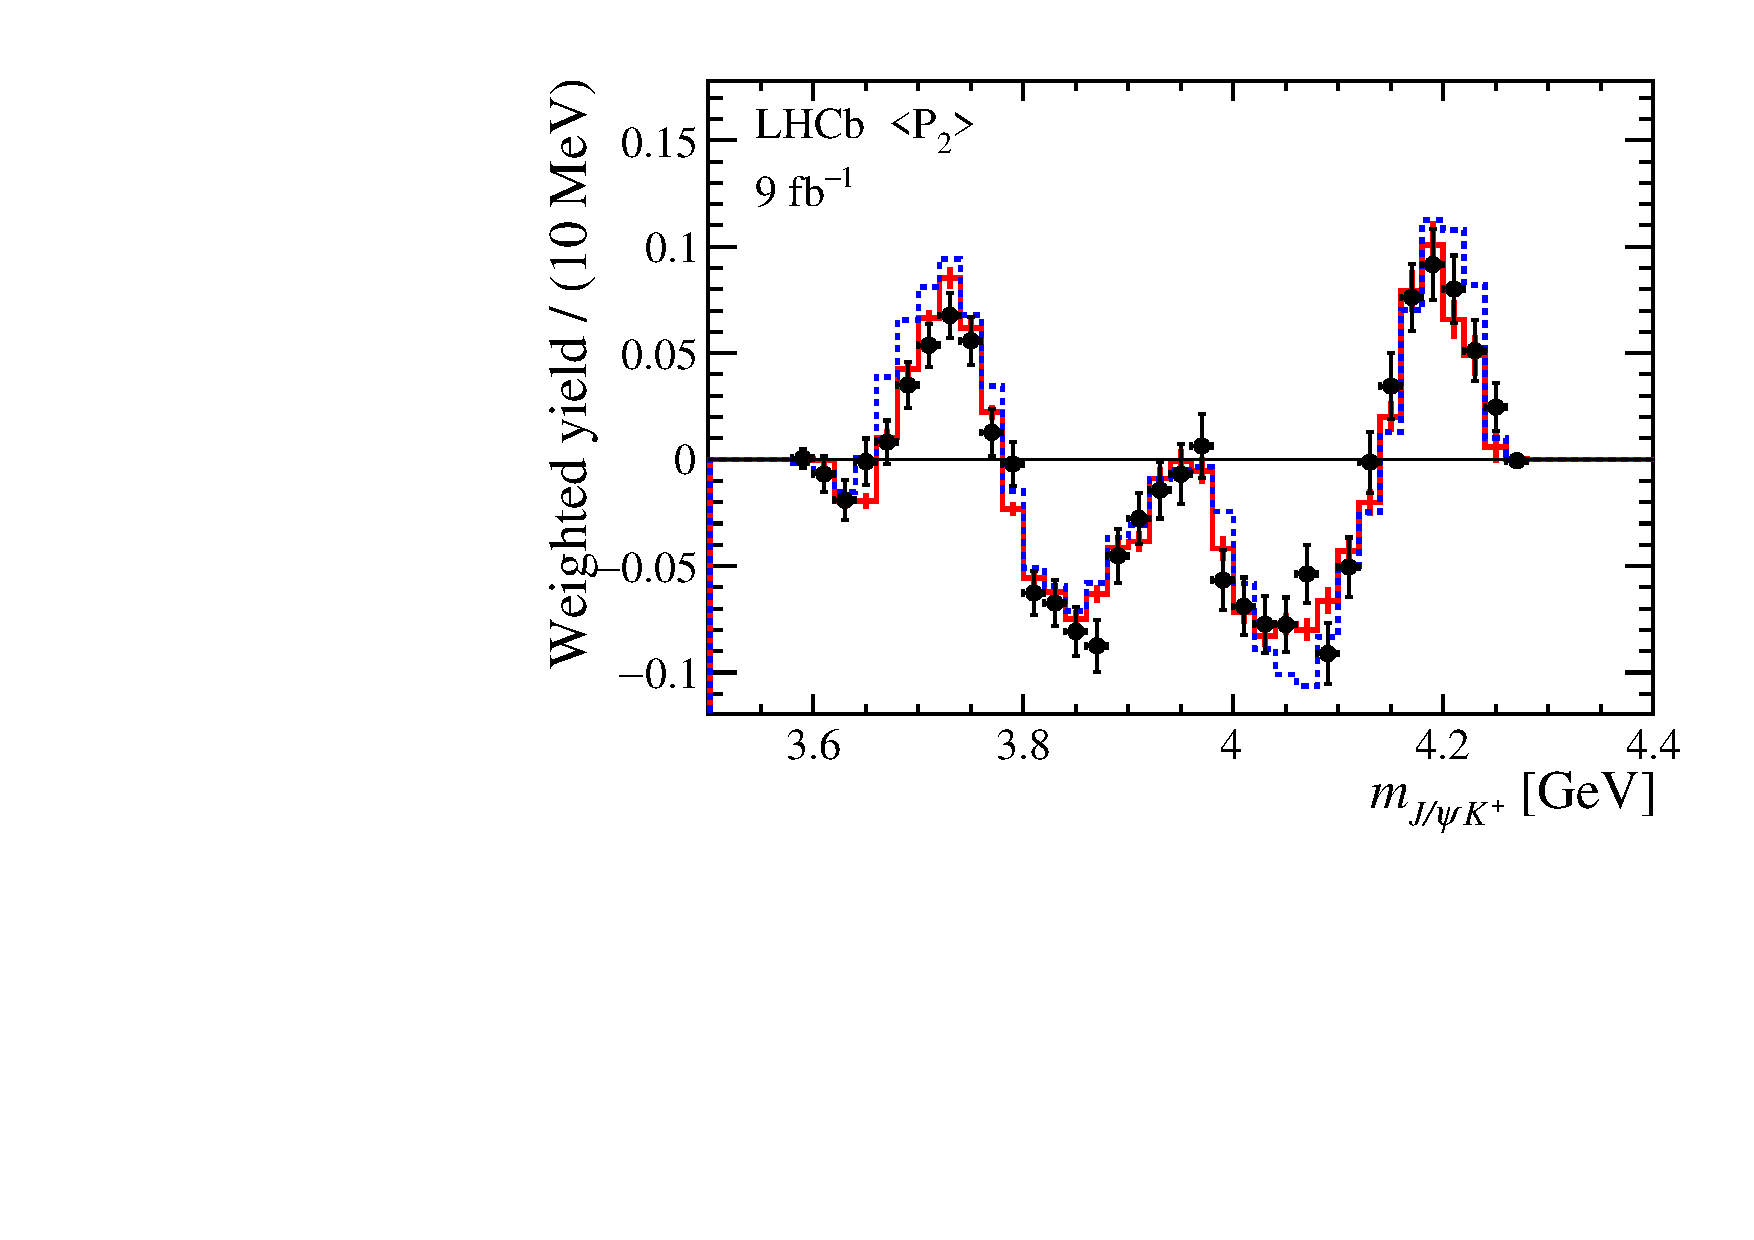
\includegraphics[width=0.33\textwidth]{Figures/03_Zcs/app_moments/shy1z2}
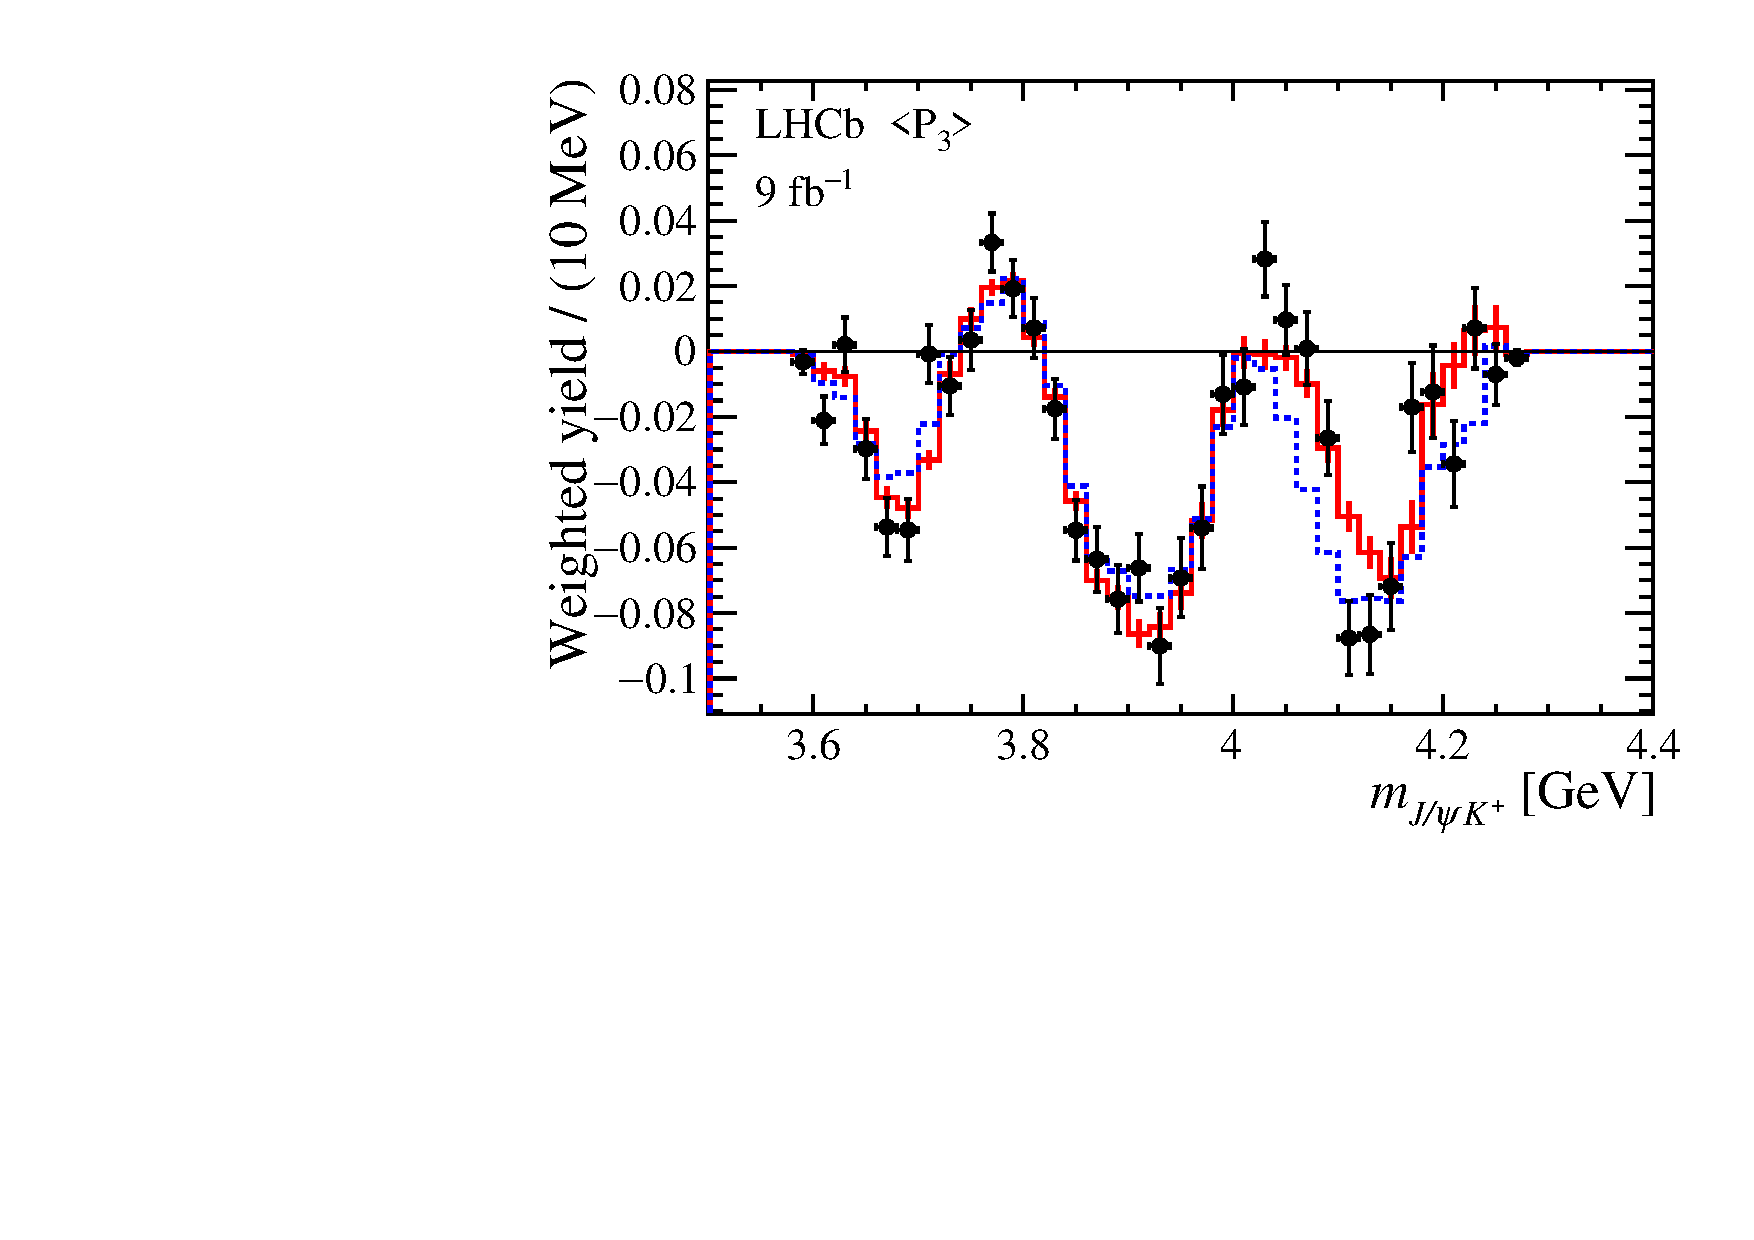
\includegraphics[width=0.33\textwidth]{Figures/03_Zcs/app_moments/shy1z3}%
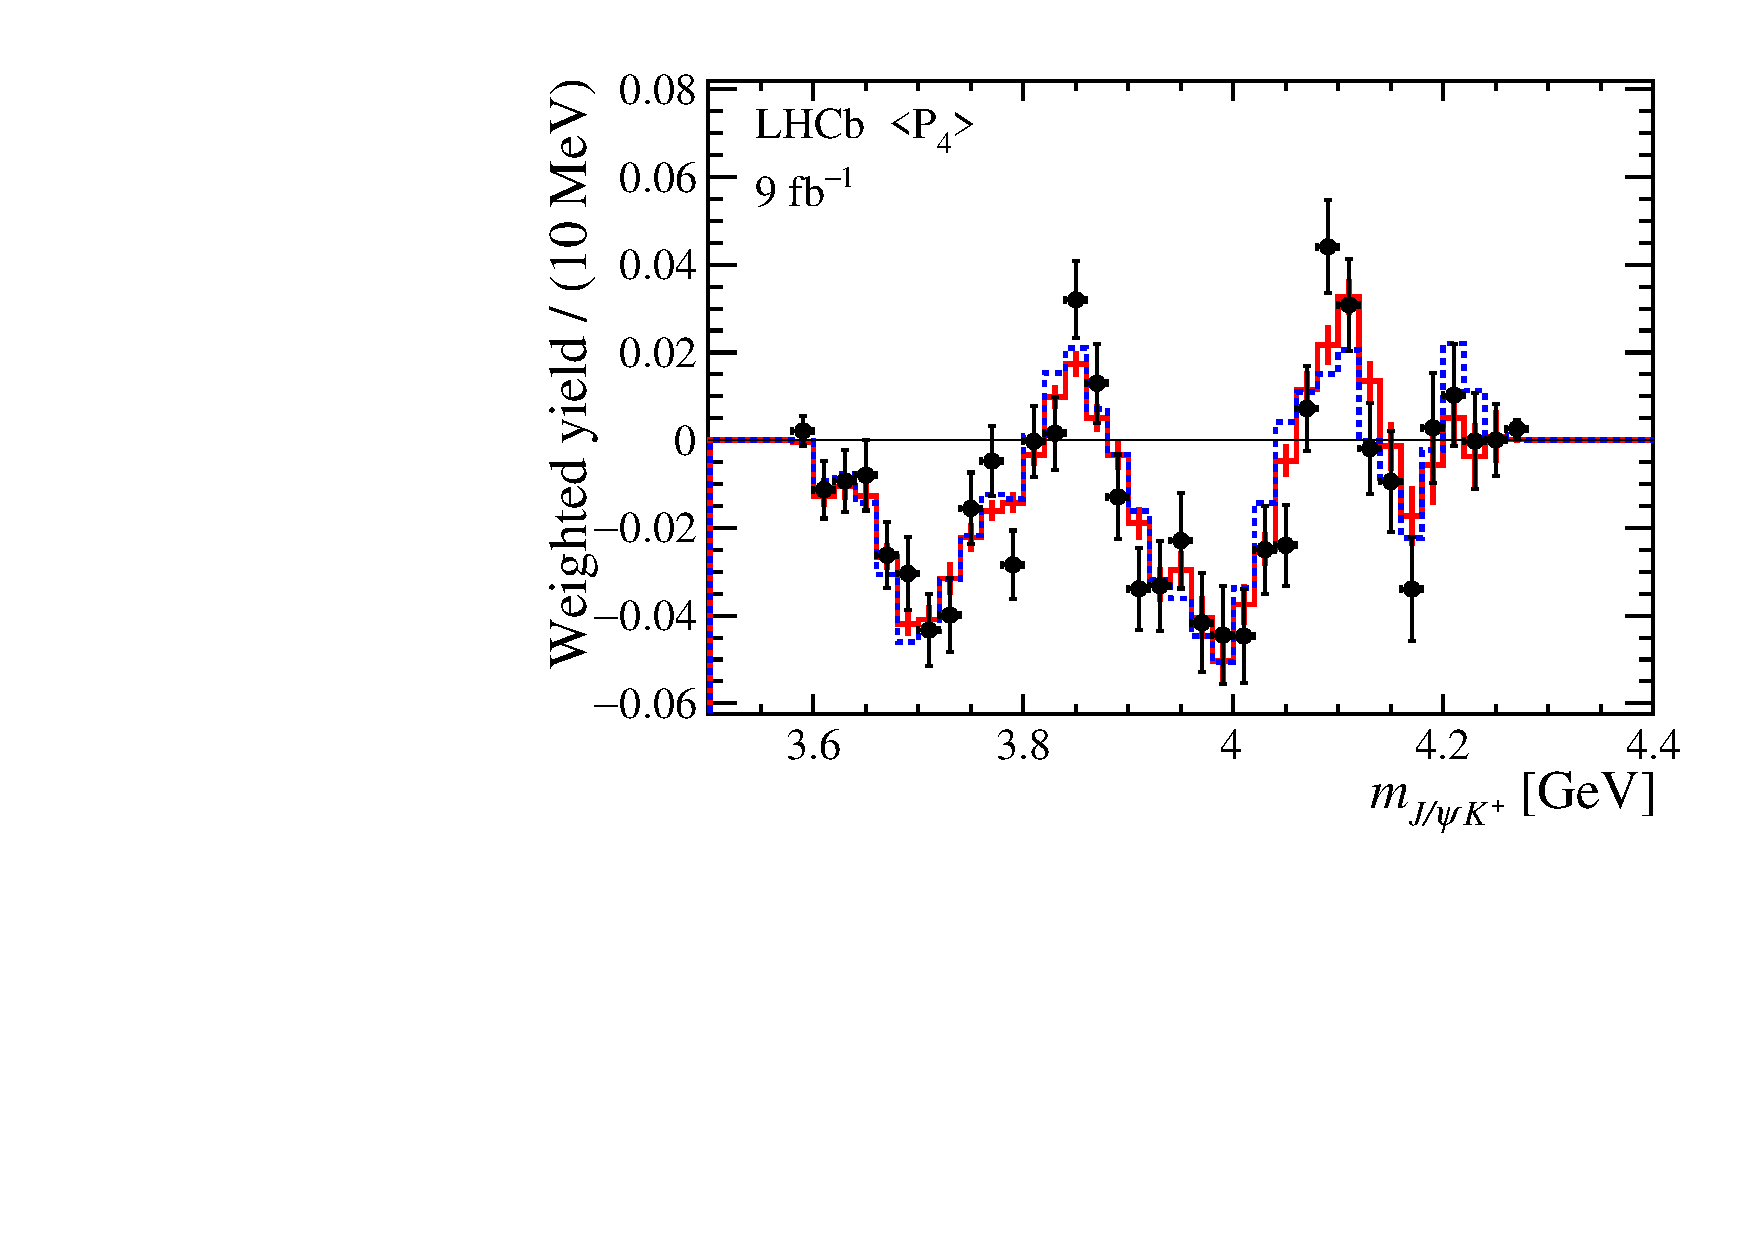
\includegraphics[width=0.33\textwidth]{Figures/03_Zcs/app_moments/shy1z4}%
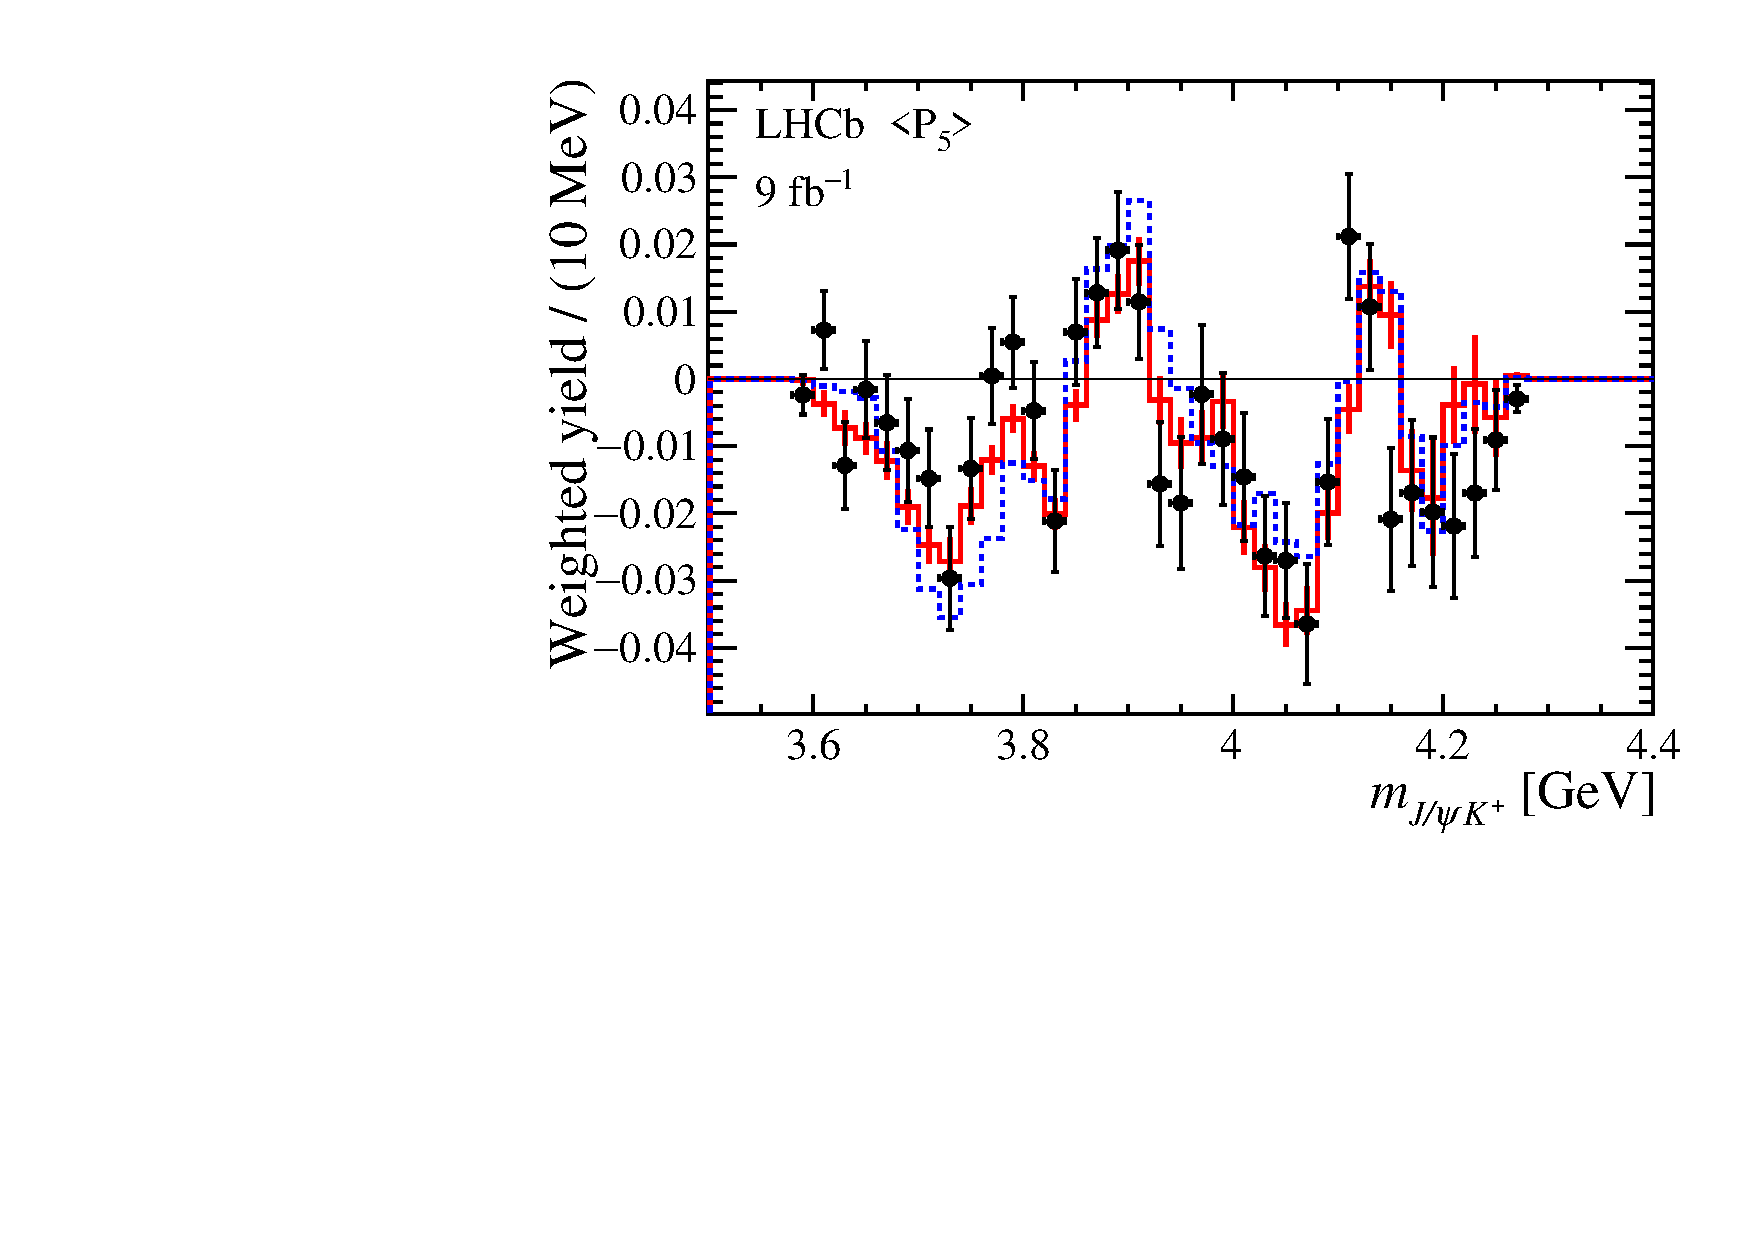
\includegraphics[width=0.33\textwidth]{Figures/03_Zcs/app_moments/shy1z5}
\caption{Angular moments of $\jpsi K$ helicity angle as a function of $\mfk$ compared between the background subtracted data, and PDFs from run1 model (blue dashed) and the nominal model (red solid). The $\chi^2/$nbin for the fit of nominal model (run1 model) are 77(138)/69, 50(108)/35, 30(75)/35, 60(81)/35, 31(41)/35, 44(68)/35 for order from 0 to 5, respectively.}
\label{mom5z}
\end{figure}



\section{Model-independent}

\label{sec:app:MI}
To cross-check the results obtained with the Breit-Wigner sum approach, 
we replace selected partial waves, 
one at a time, 
with a model-independent (MI) description of the complex amplitude describing the mass dependence.
We first investigate $J^P=1^+$ $Z\to\jpsi K$ partial wave in which we use two BW poles in the nominal model.
The other resonances are described by BW as done in the nominal fit, 
since the data are unable to constraint many waves in MI approach at the same time. i
The BW functions for the two $1^+$ $Z$'s are replaced by complex numbers $c_i$,
where $i=1,...,25$, 
representing this wave in 27\mev bins of $\mjk$. 
The MI amplitude at any value of $\mjk$ is returned by two cubic splines for the Real and Imaginary parts of $c_i$. 
To be more specific, the mass dependent term $R$ for a wave of $Z_j$ is reformed as
\begin{equation}
R_{Z_j}(m_{\jpsi K}) =
B'_{L_{B}^{Z_j}}(p,p_0,d) \left(\frac{p}{M_{B}}\right)^{L_{B}^{Z_j}} \, c_i(\mjk)
\label{SUPeq:resmi}
\end{equation}
Here $p_0$ is calculated using the center mass of $\mjk$ (\ie $({\mjk}^{\rm min}+{\mjk}^{\rm max})/2$), 
and $L_{B}$ takes the lowest allowed value. 
Comparing the above equation with Eq.~(\ref{SUPeq:resshape}), 
the MI complex amplitude include BW function and the Blatt-Weisskopf function of resonance decay.

To simplify, 
one MI is used to represent all $LS$ partial waves of $1^+$ $Z$ contributions. 
We compare this fit and the model-dependent nominal BW-sum results 
for the amplitude squared and complex phase in a function of $\mjk$ in Fig.~\ref{fig:MIZ1P}. 
The corresponding Argand plot is shown in Fig.~\ref{fig:ArgZ1p}. 
The MI study confirms that two $Z$ states are needed in $1^+$ partial wave.

\begin{figure*}[hbtp]
\centering
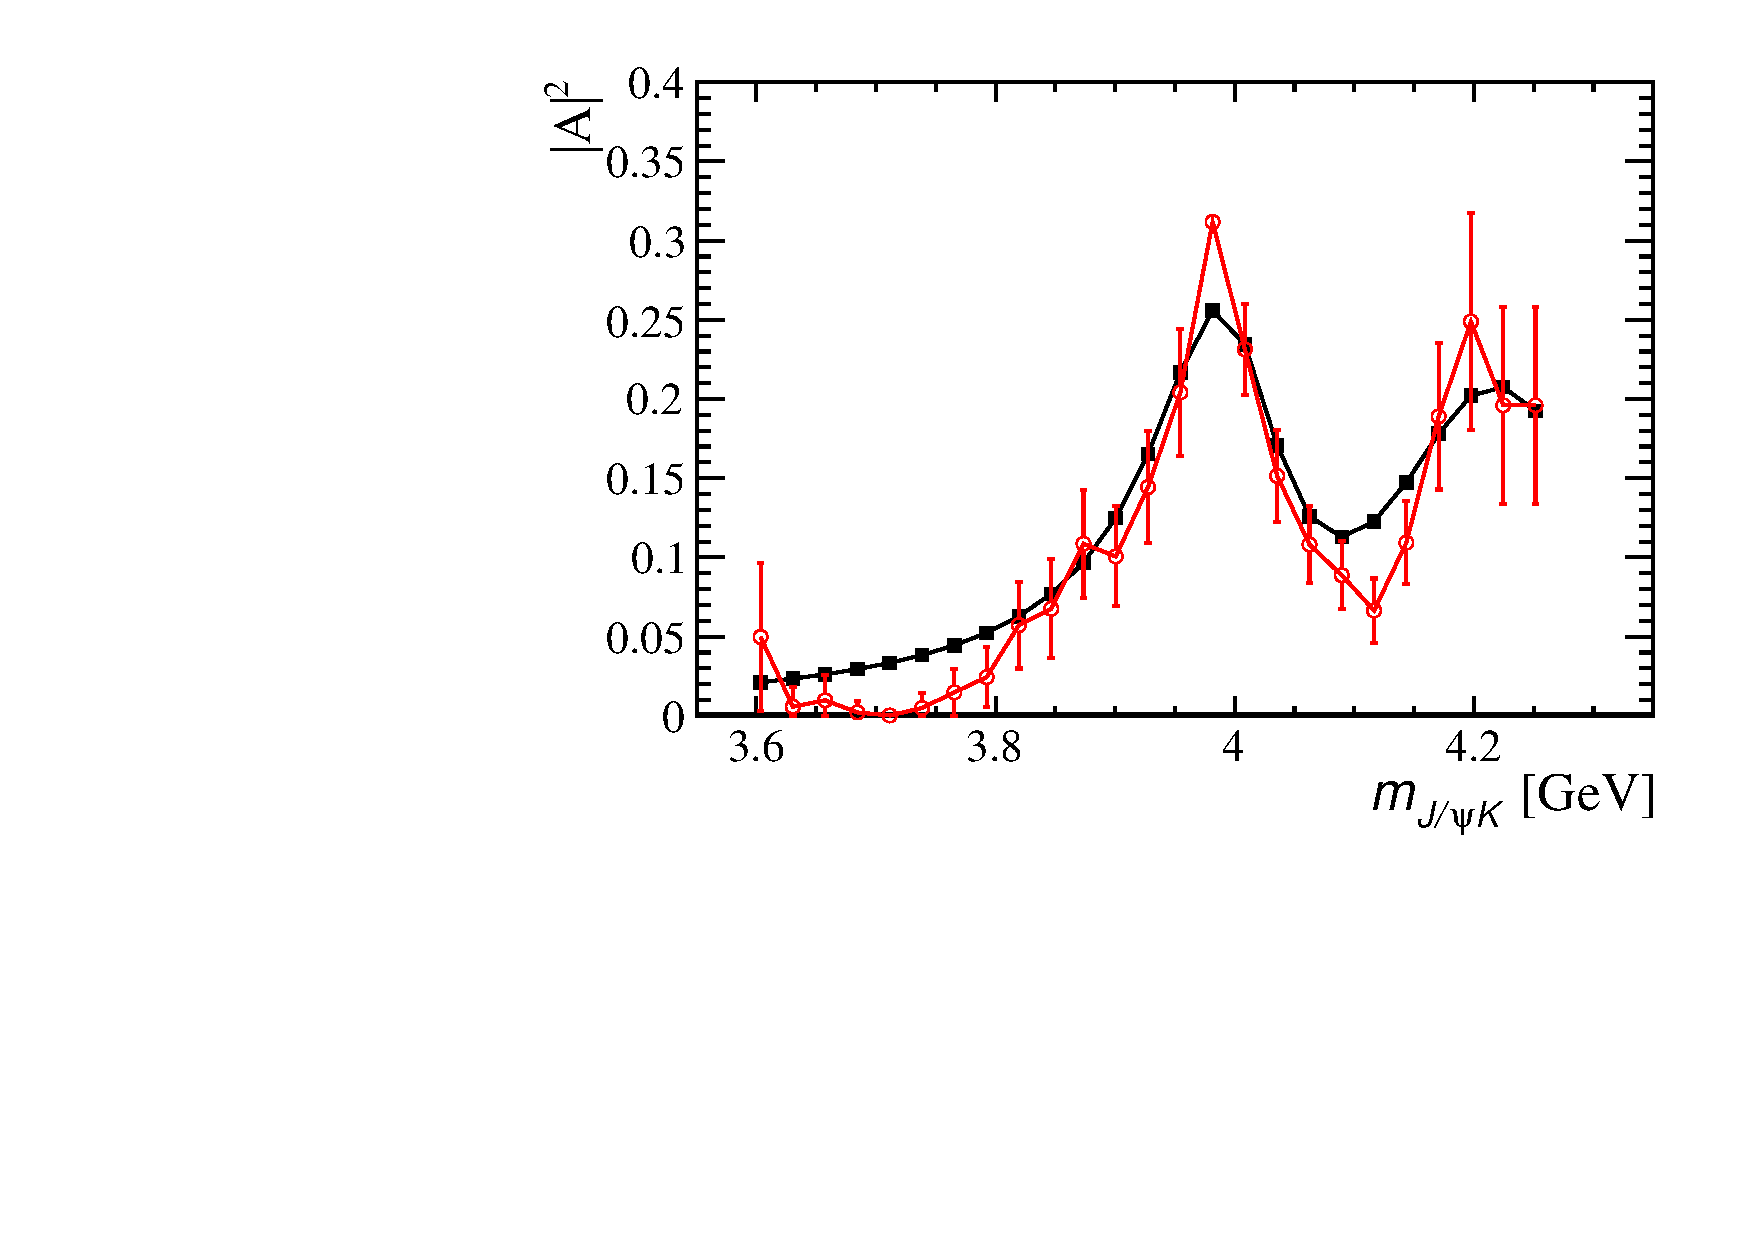
\includegraphics[width=0.4\textwidth]{Figures/03_Zcs/app_MI/A2_Z1P}%
\put(-35,105) {\textrm{\small \bf(a)}}%
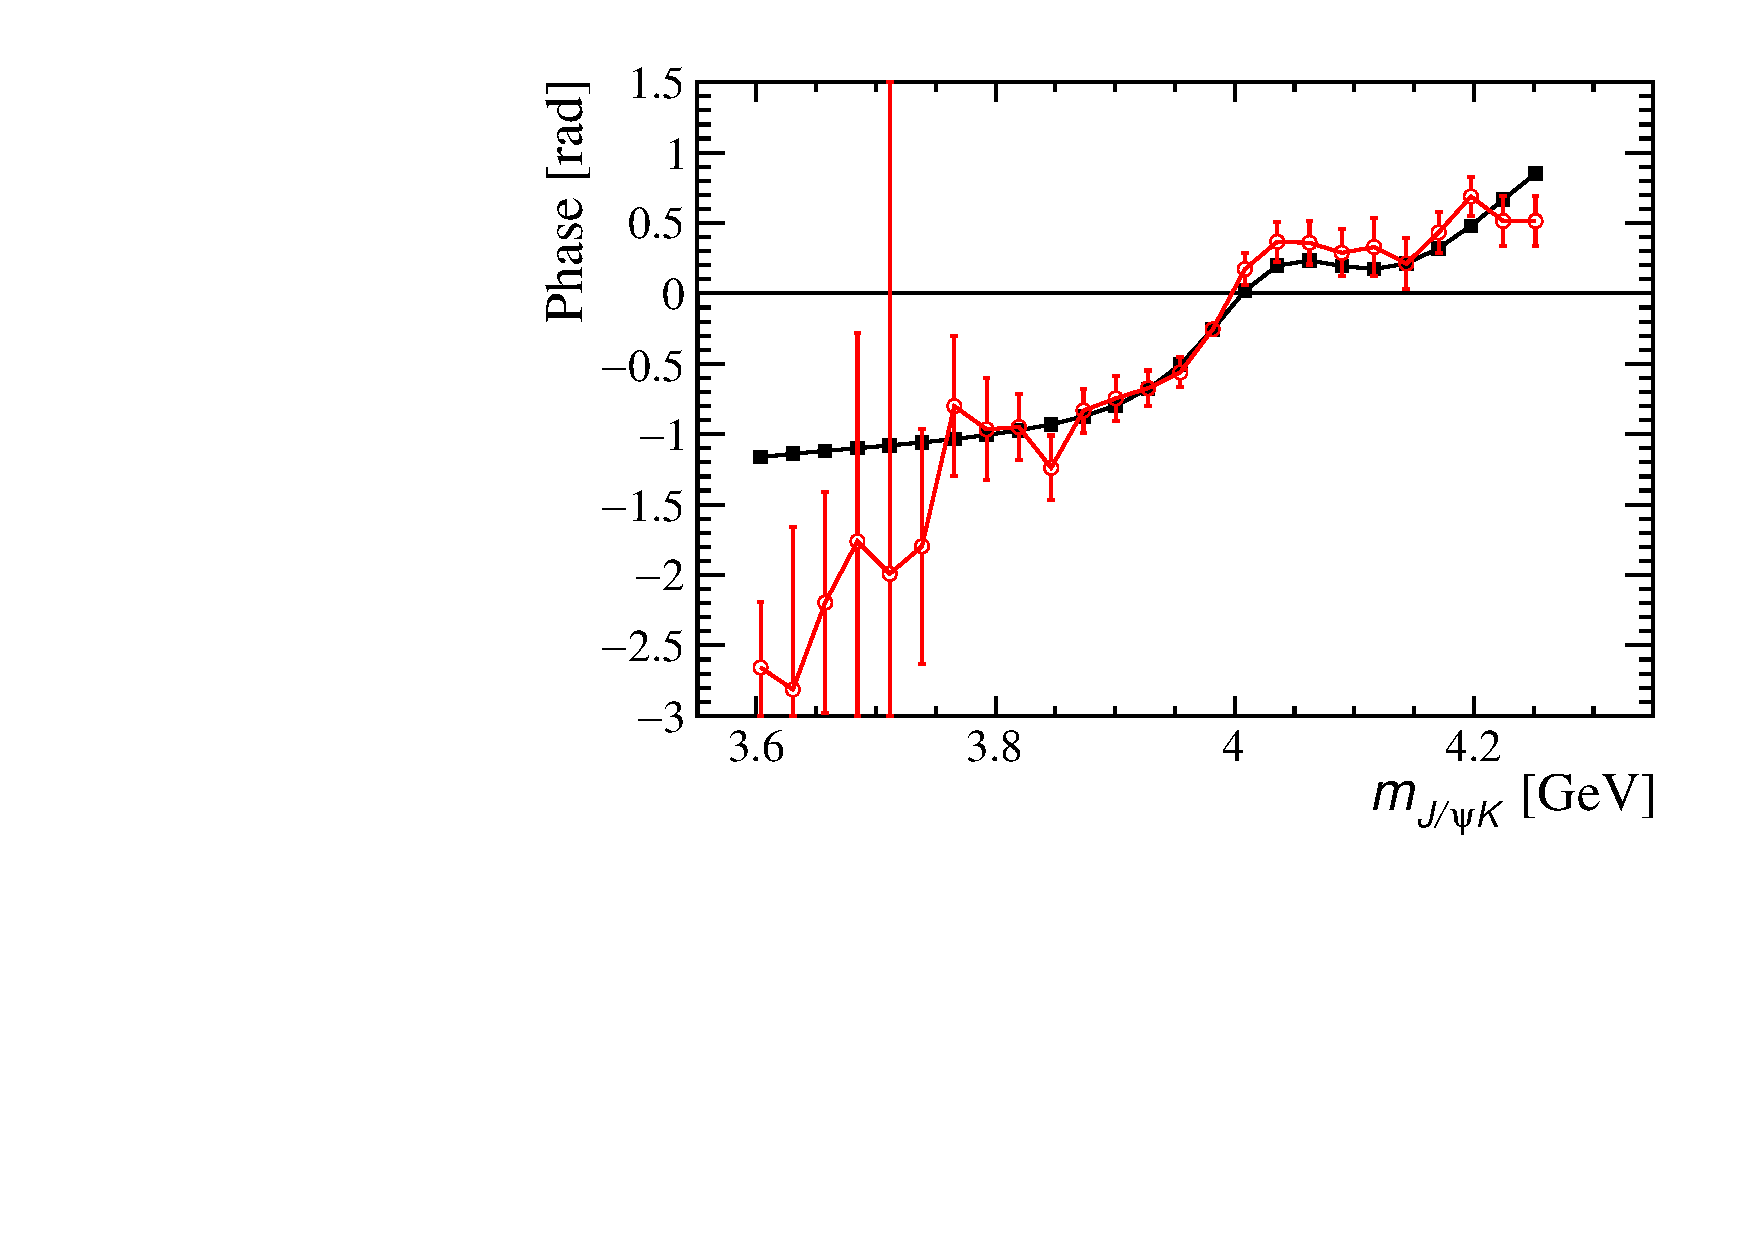
\includegraphics[width=0.4\textwidth]{Figures/03_Zcs/app_MI/Ph_Z1P}
\put(-35,105){\textrm{\small \bf(b)}}
\caption{(a) Amplitude squared and (b) phase motion for $1^+$ $Z$ wave obtained from the model-independent method (red open) and the nominal BW-sum fit (black solid).
The BW-sum model has poles at $M_0-i\Gamma_0/2=4003-i\,131/2$ and $4216-i\,233/2$ \mev, 
obtained from sum of the lowest $L$ waves for a reference.}
\label{fig:MIZ1P}
\end{figure*}

\begin{figure}[hbtp]
\centering
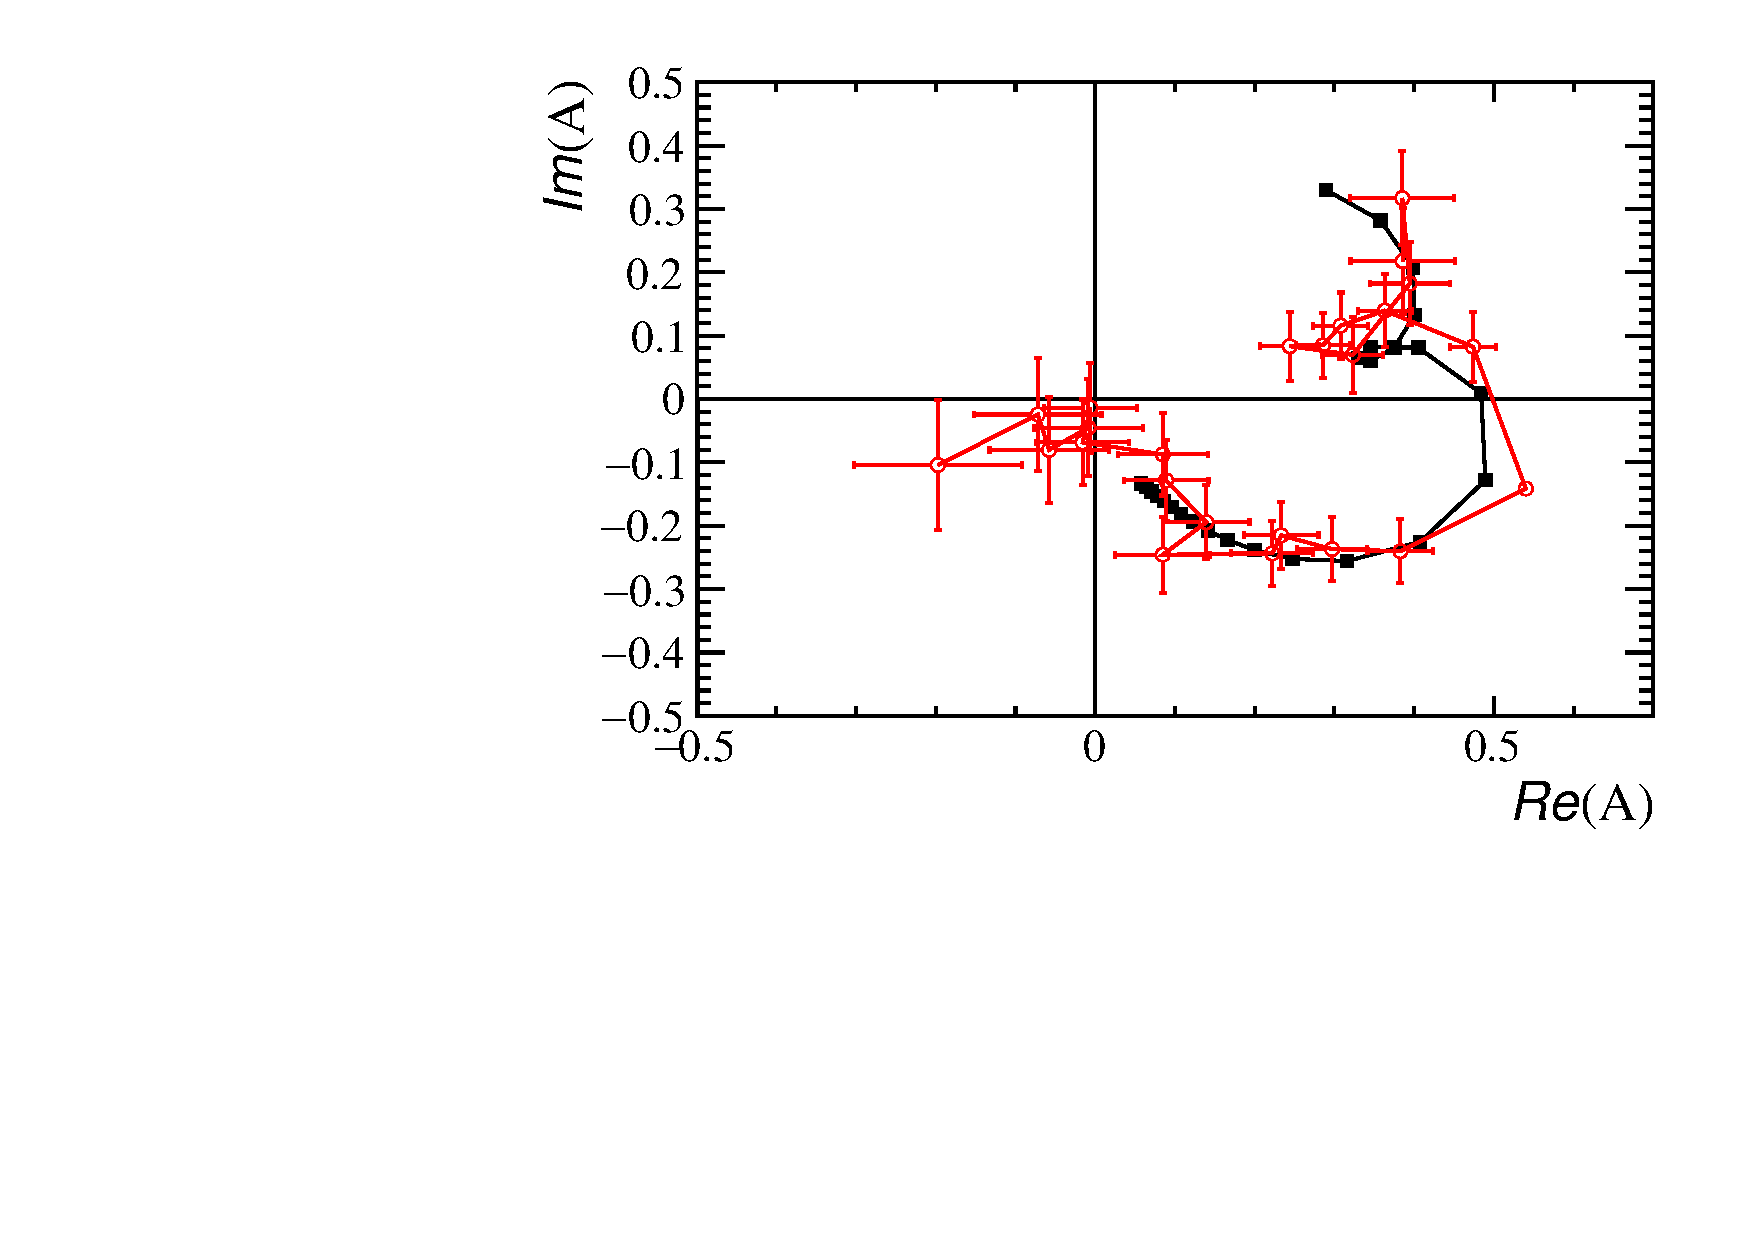
\includegraphics[width=0.4\textwidth]{Figures/03_Zcs/app_MI/Argand_Z1P}
\caption{Argand plot of $1^+$ $Z$ waves obtained from the model-independent method (red  open) and the nominal BW-sum fit (black solid). 
The BW-sum model has poles at $M_0-i\Gamma_0/2=4003-i\,131/2$ and $4216-i\,233/2$ \mev, 
obtained from sum of the lowest $L$ waves for a reference.}\label{fig:ArgZ1p}
\end{figure}

\begin{figure*}[hbtp]
\centering
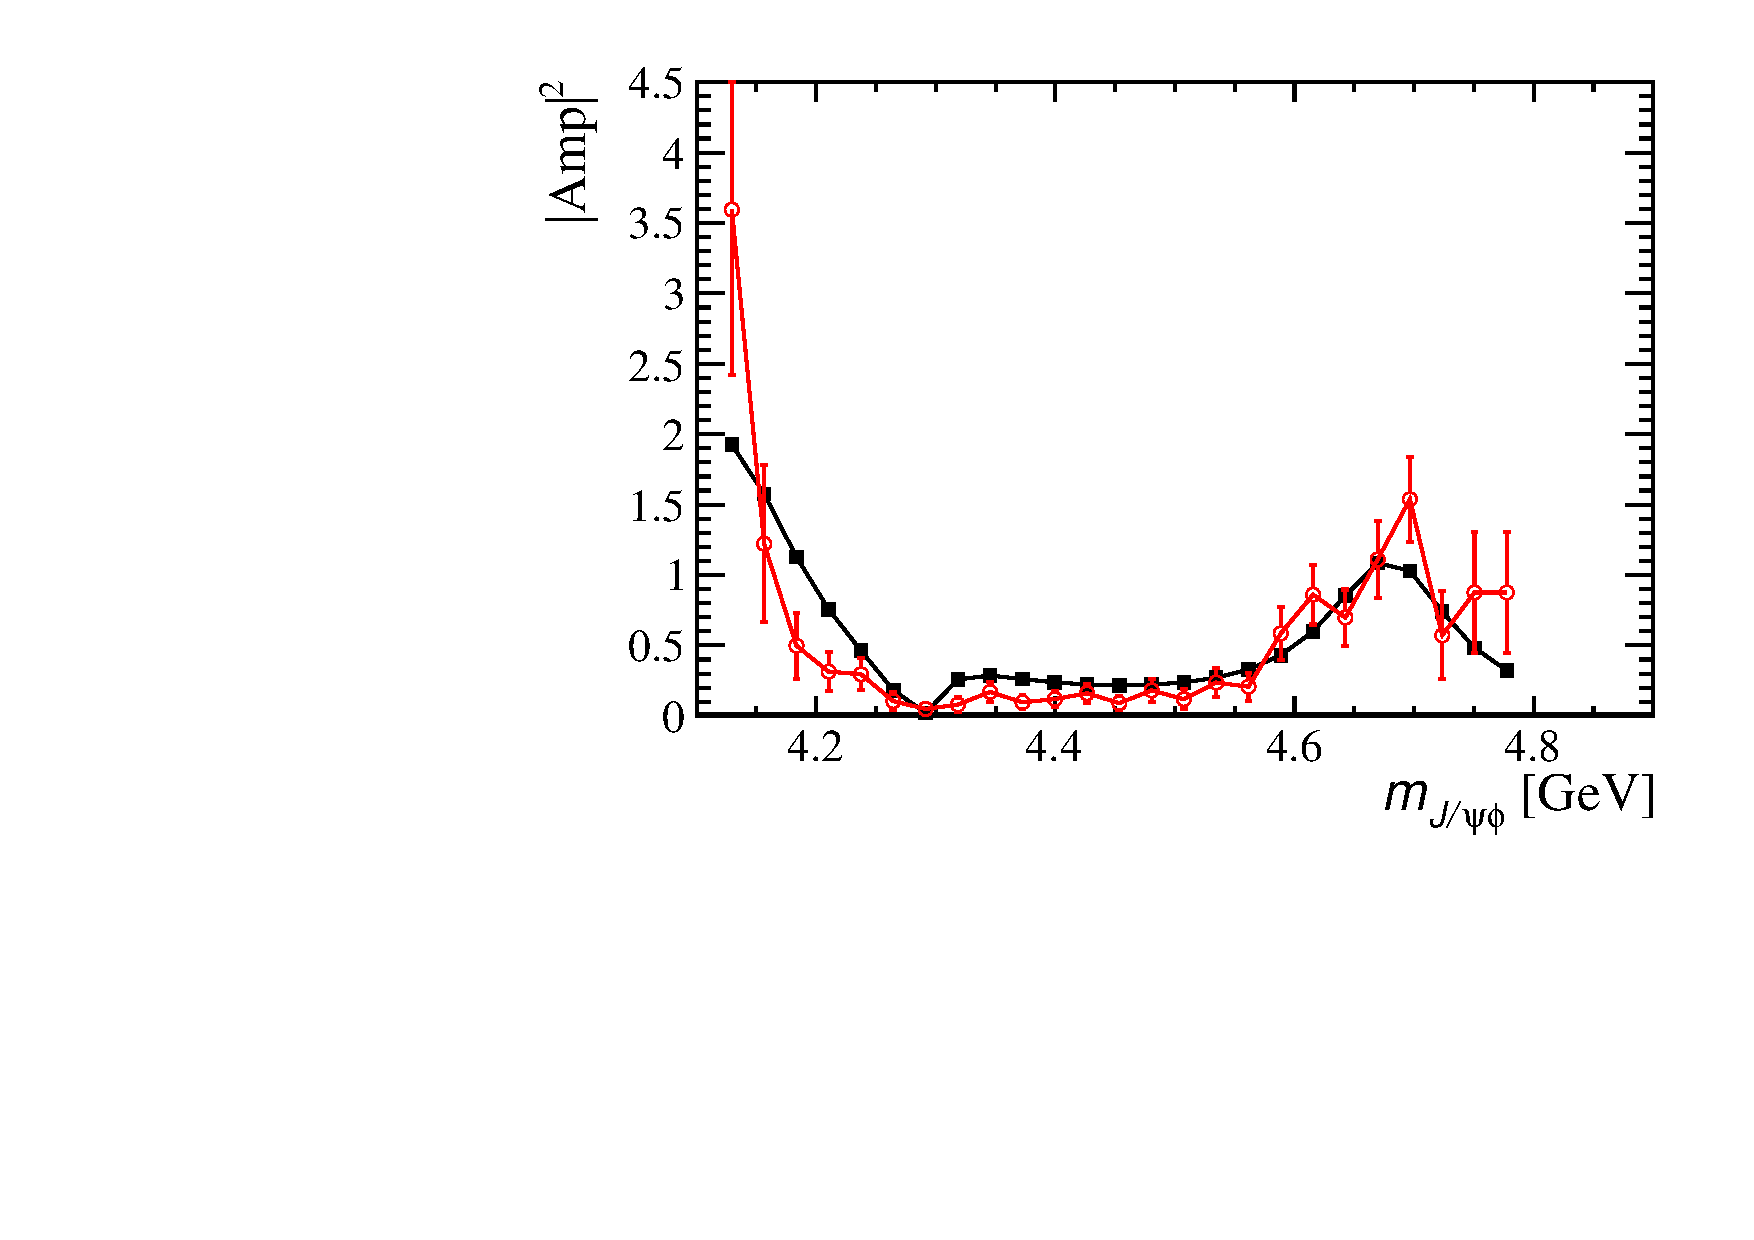
\includegraphics[width=0.4\textwidth]{Figures/03_Zcs/app_MI/A2_X1P_same}%
\put(-35,105) {\textrm{\small \bf(a)}}%
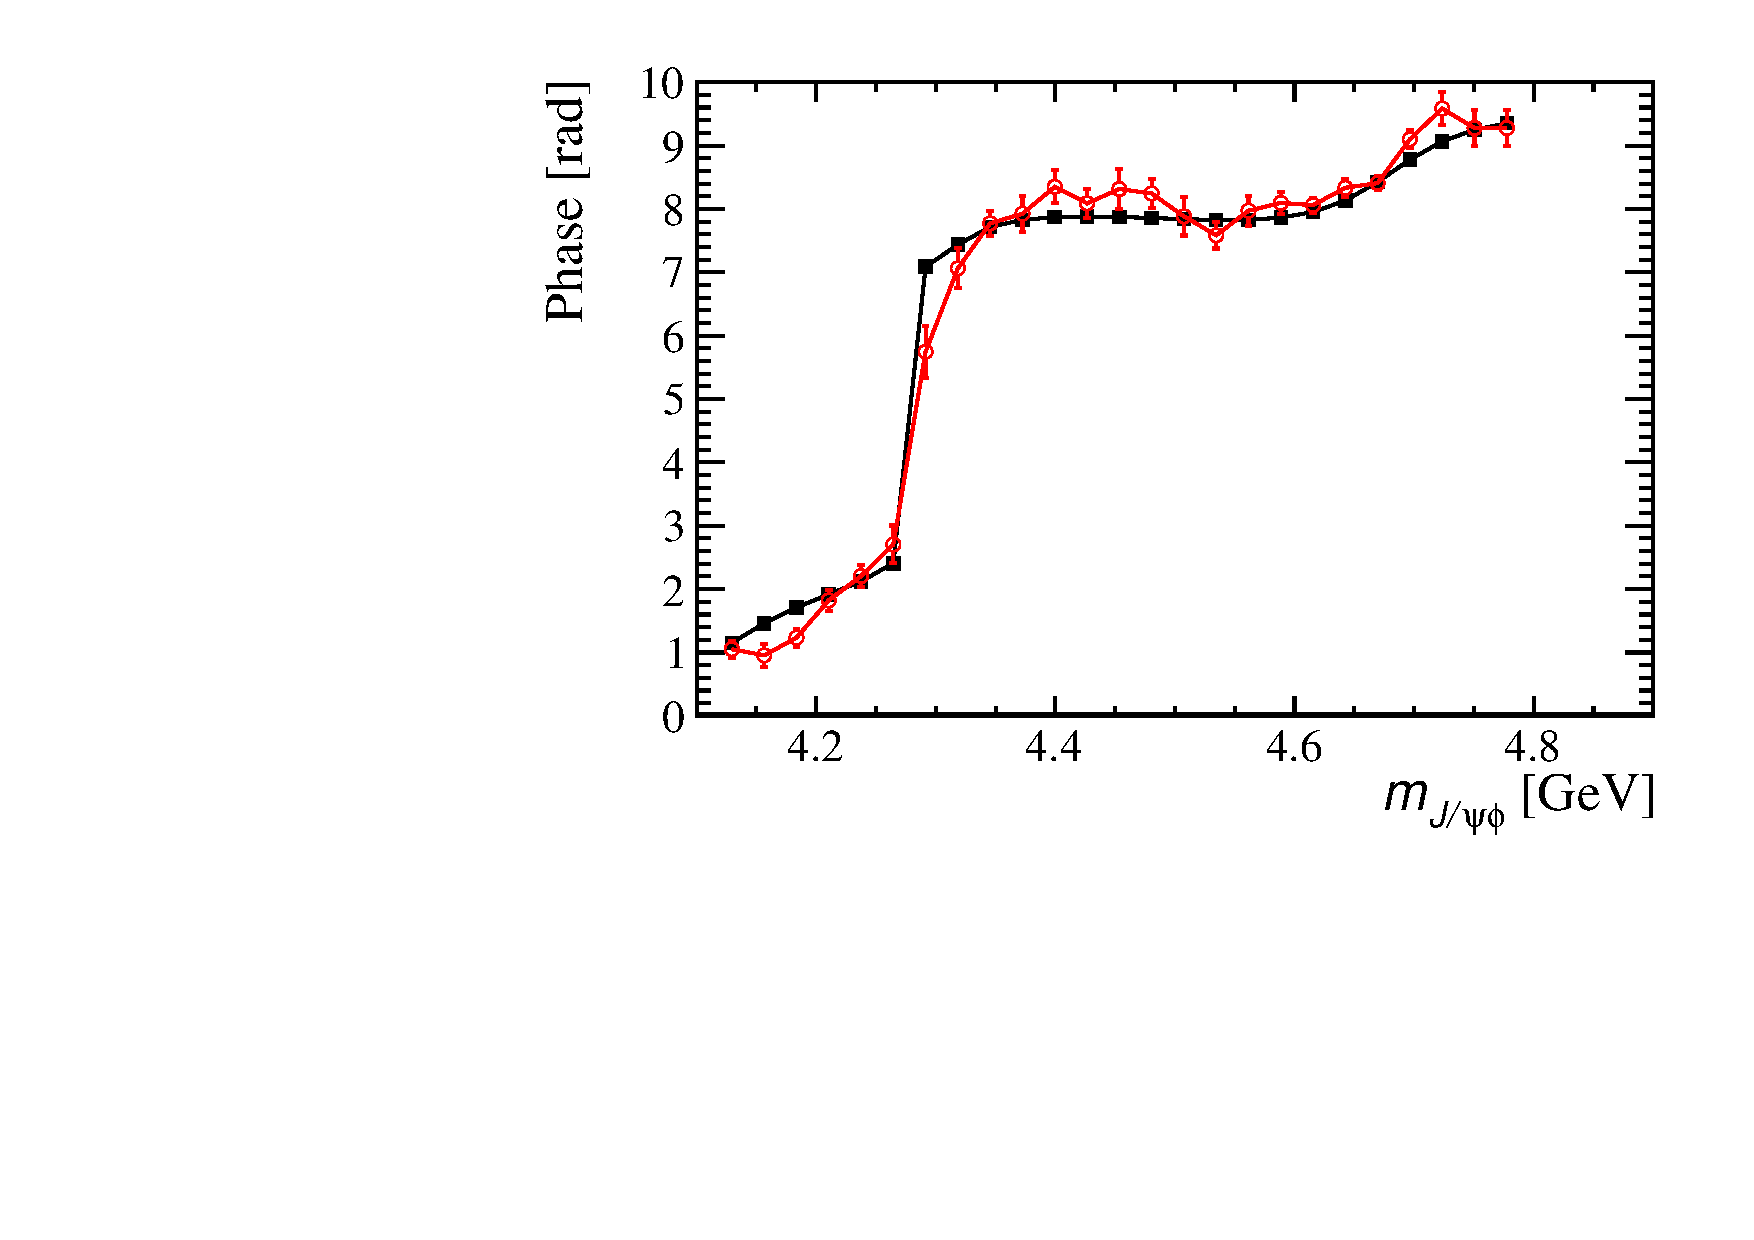
\includegraphics[width=0.4\textwidth]{Figures/03_Zcs/app_MI/Ph_X1P_same}
\put(-35,105){\textrm{\small \bf(b)}}
\caption{(a) Amplitude squared and (b) phase motion for $1^+$ $X$ lowest $L$ wave obtained from the model-independent method (red  open) and the nominal BW-sum fit (black solid).
The BW-sum model has poles at $M_0-i\Gamma_0/2=4118-i\,162/2$, $4294-i\,53/2$ and $4684-i\,126/2$ \mev, 
obtained from sum of the lowest $L$ waves for a reference.}
\label{fig:MIX1P}
\end{figure*}

\begin{figure*}[hbtp]
\centering
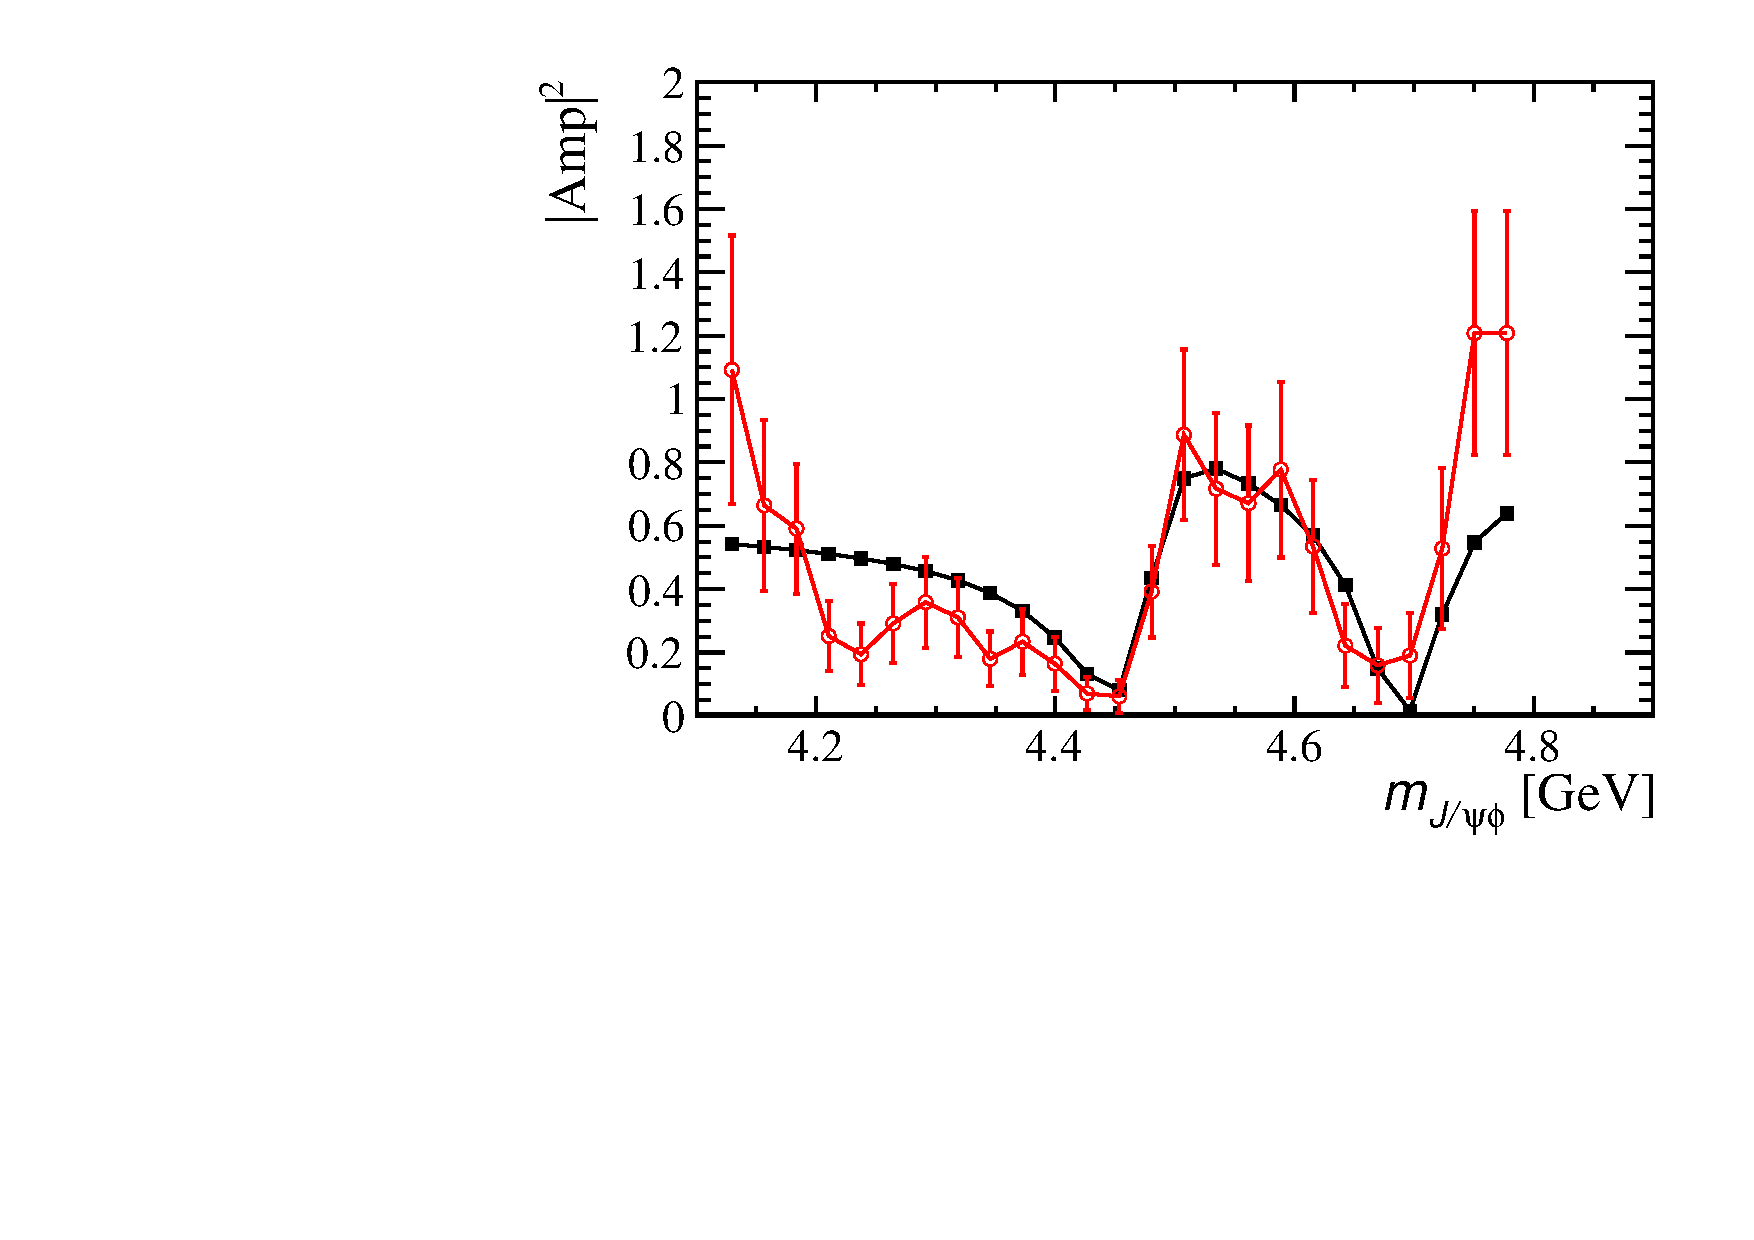
\includegraphics[width=0.4\textwidth]{Figures/03_Zcs/app_MI/A2_X0P_same}%
\put(-35,105) {\textrm{\small \bf(a)}}%
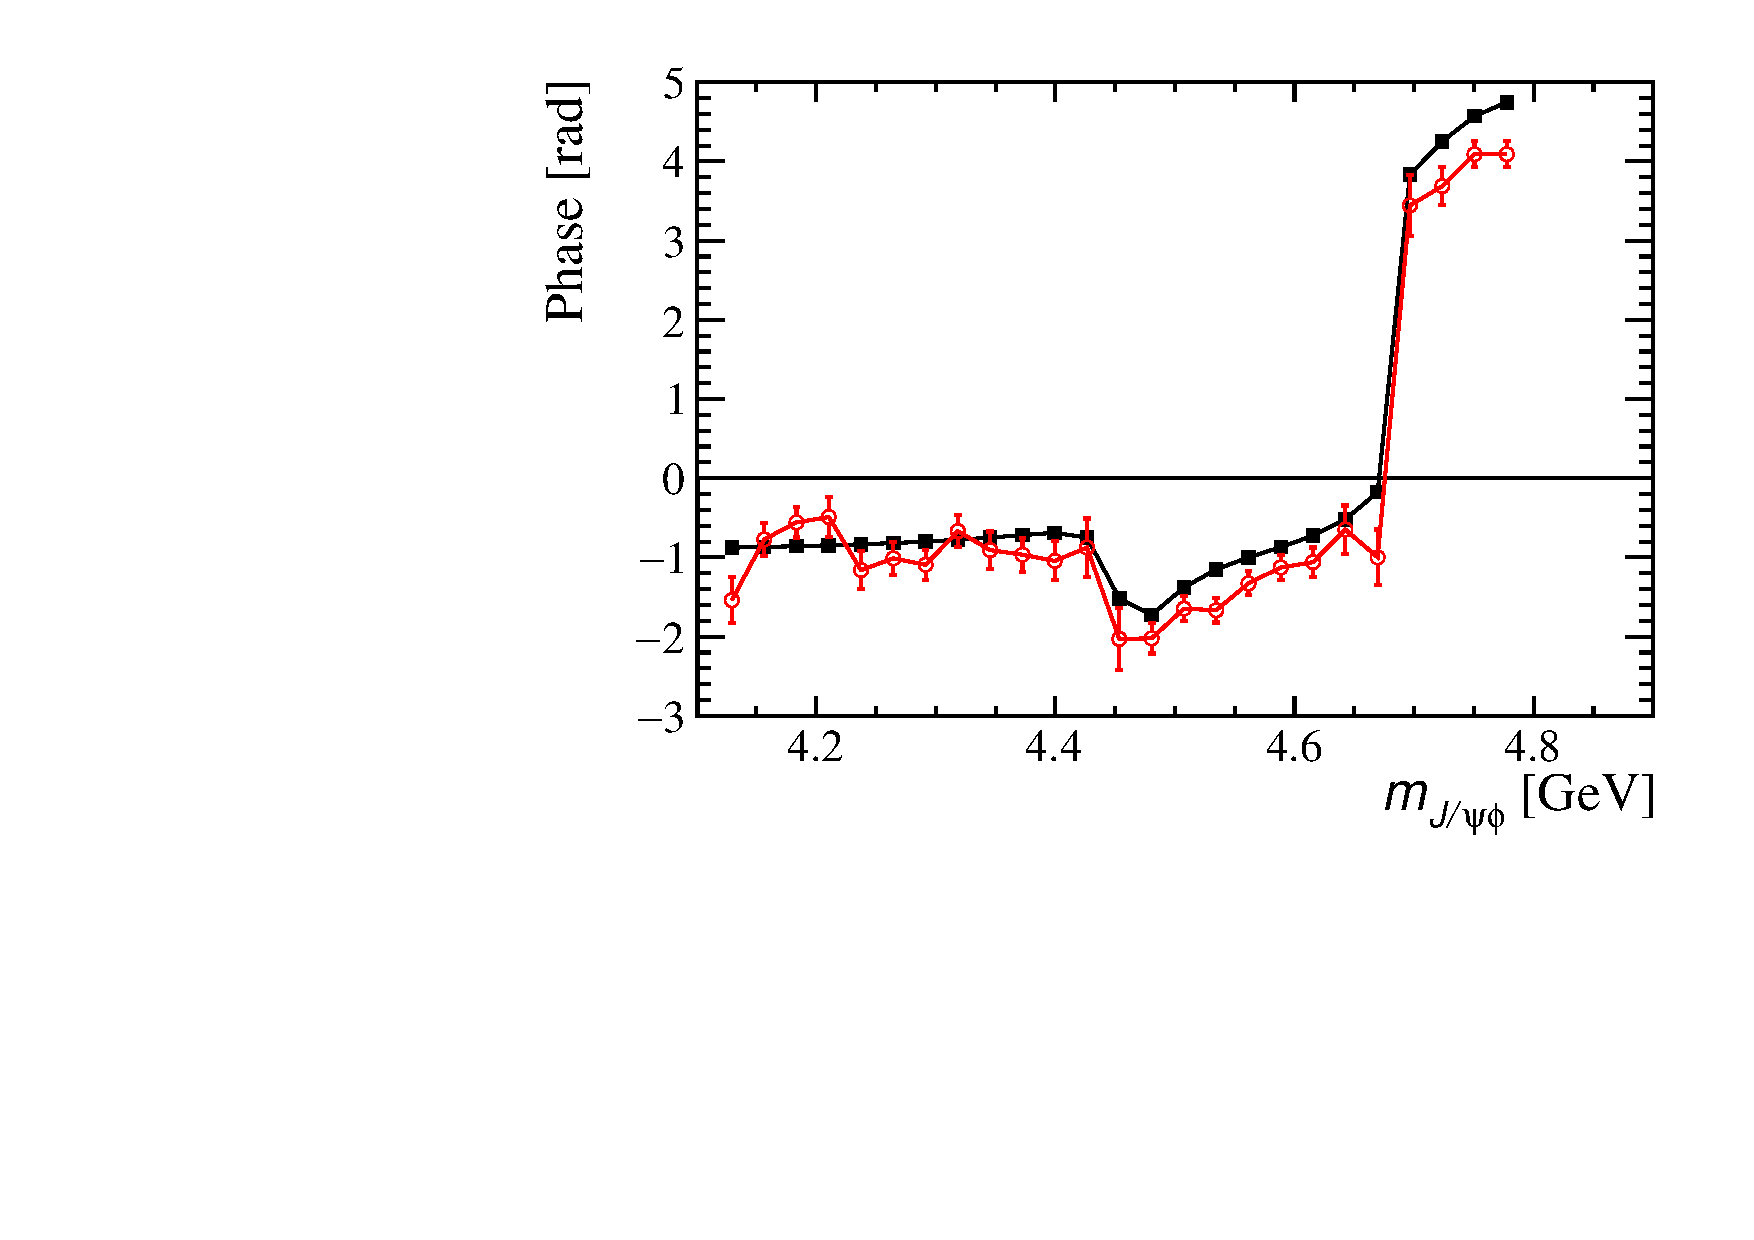
\includegraphics[width=0.4\textwidth]{Figures/03_Zcs/app_MI/Ph_X0P_same}
\put(-35,105){\textrm{\small \bf(b)}}
\caption{(a) Amplitude squared and (b) phase motion for $0^+$ $X$ lowest $L$ wave obtained from the model-independent method (red  open) and the nominal BW-sum fit (black solid).
The BW-sum model has poles at $M_0-i\Gamma_0/2=4474-i\,77/2$, $4694-i\,87/2$ \mev and the NR contribution, 
obtained from sum of the lowest $L$ waves for a reference.}
\label{fig:MIX0P}
\end{figure*}

\begin{figure}[hbtp]
\centering
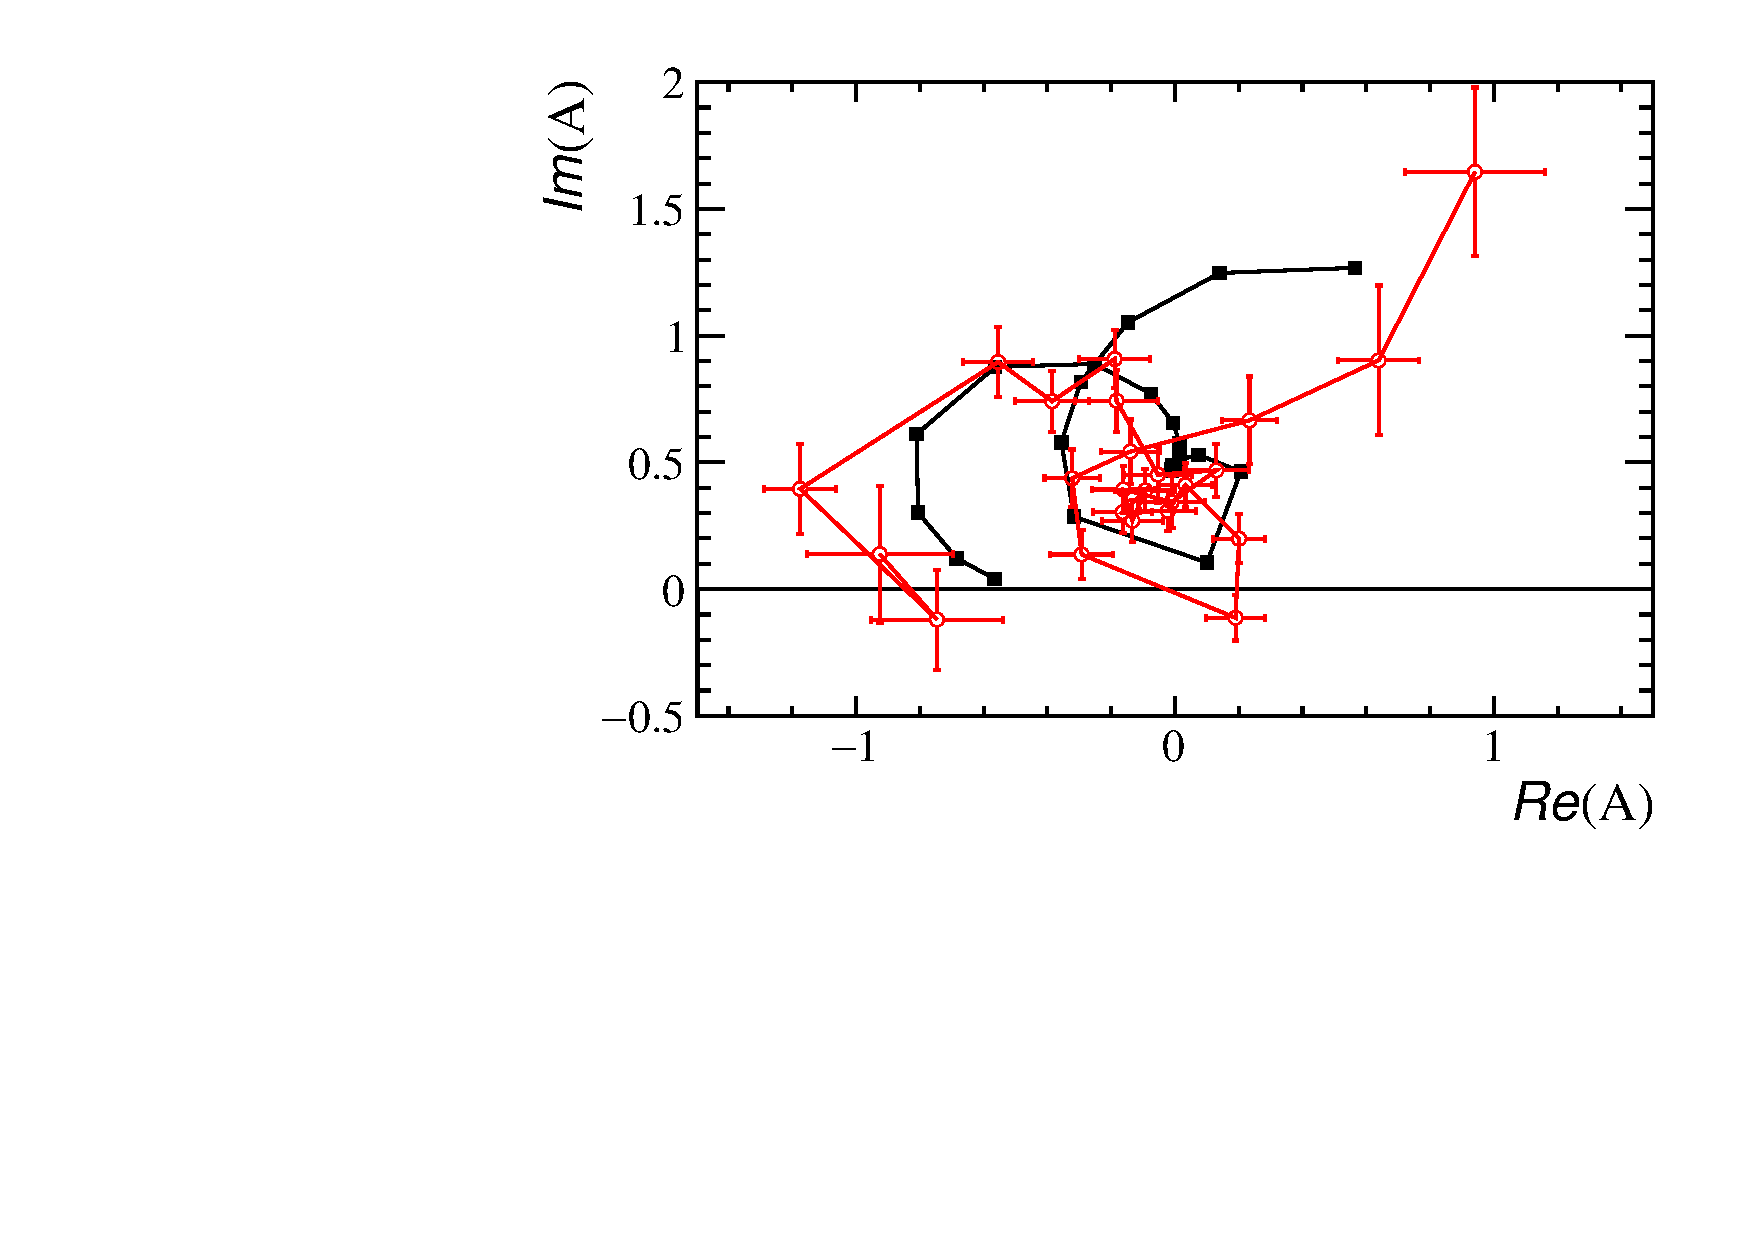
\includegraphics[width=0.4\textwidth]{Figures/03_Zcs/app_MI/Argand_X1P_same}%
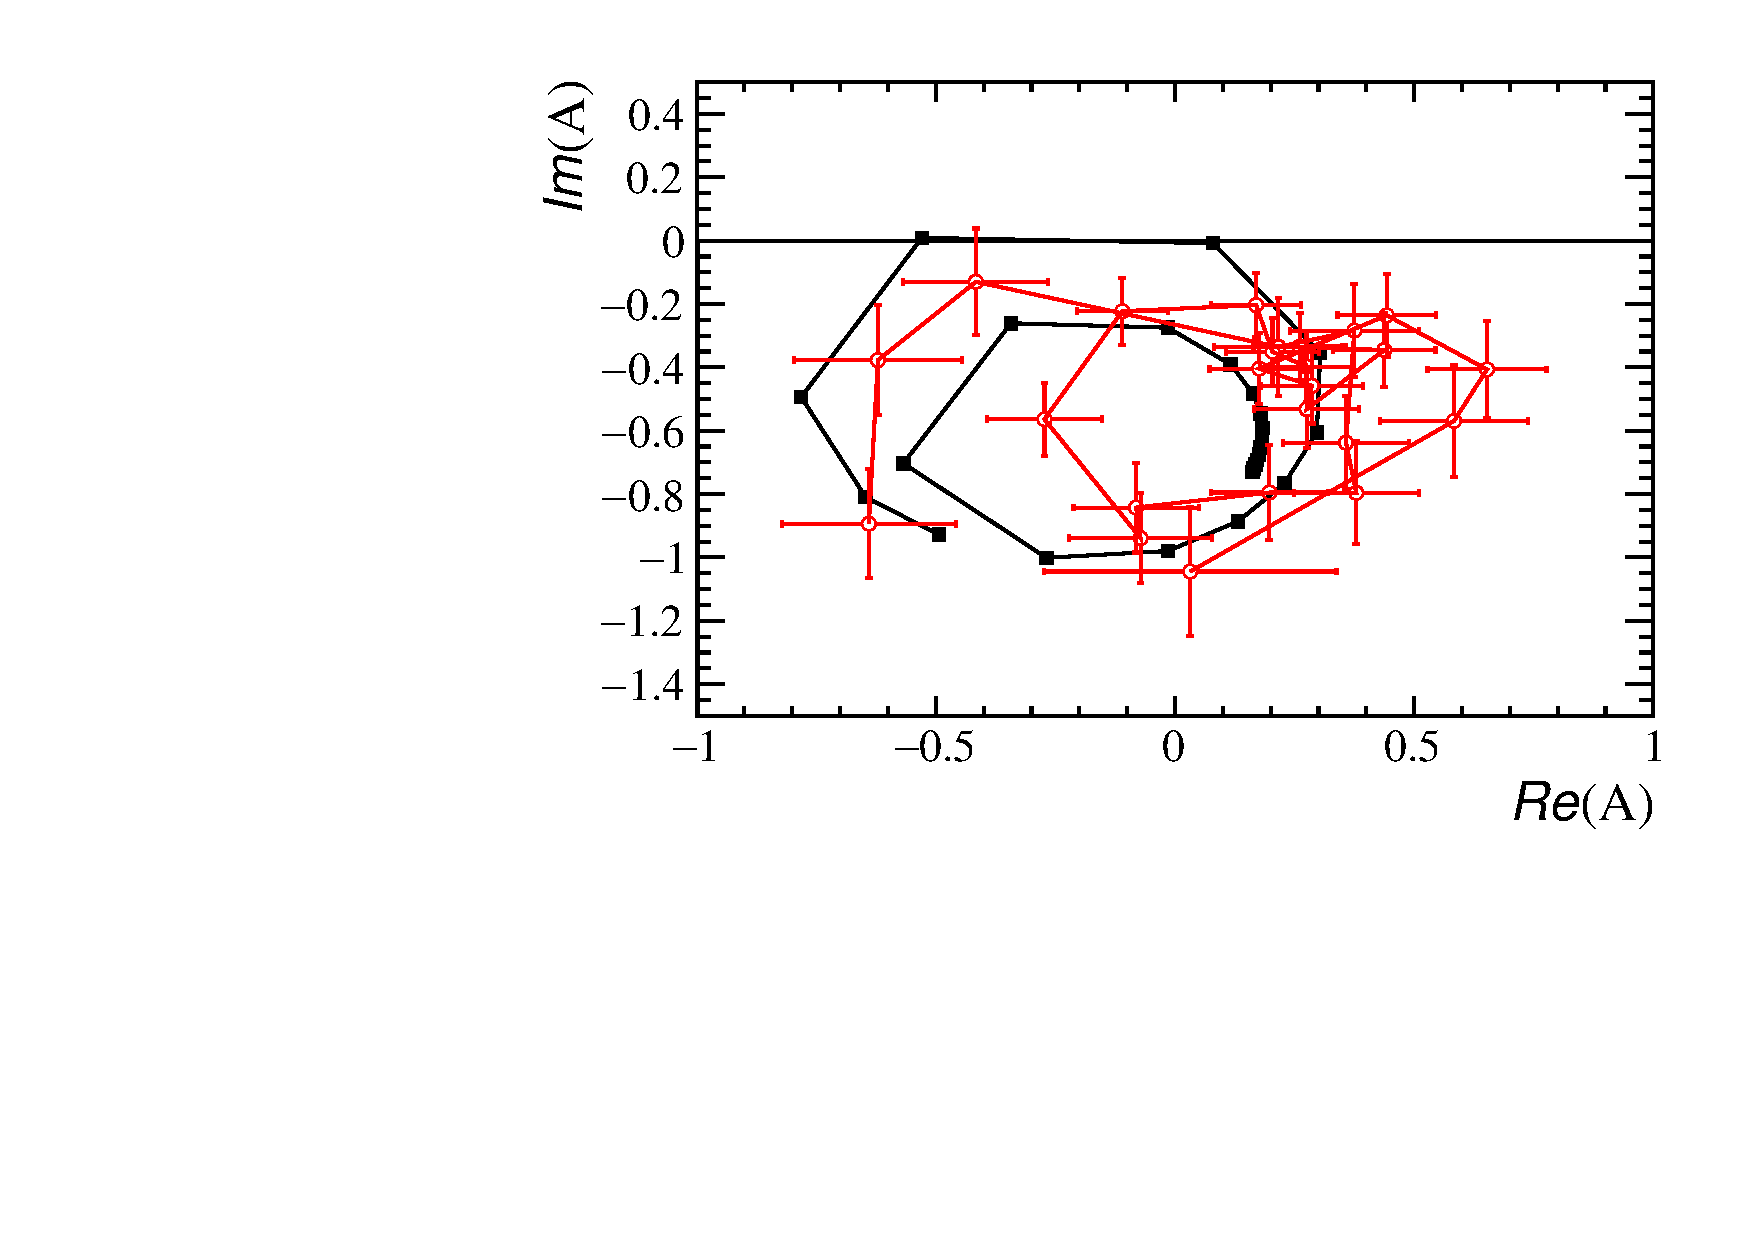
\includegraphics[width=0.4\textwidth]{Figures/03_Zcs/app_MI/Argand_X0P_same}
\caption{(Left) Argand plot of $1^+$ $X$ waves obtained from the model-independent method (red  open) and the nominal BW-sum fit (black solid). 
The BW-sum model has poles poles at $M_0-i\Gamma_0/2=4118-i\,162/2$, $4294-i\,53/2$ and $4684-i\,126/2$ \mev, 
obtained from sum of the lowest $L$ waves for a reference. 
(Right) Argand plot of $0+$ $X$ waves obtained from the model-independent method (red  open) 
and the nominal BW-sum fit (black solid). 
The BW-sum model has poles poles at $M_0-i\Gamma_0/2=4118-i\,162/2$, $4294-i\,53/2$ and $4684-i\,126/2$ \mev, 
obtained from sum of the lowest $L$ waves for a reference.}\label{fig:ArgX}
\end{figure}

\begin{figure*}[hbtp]
\centering
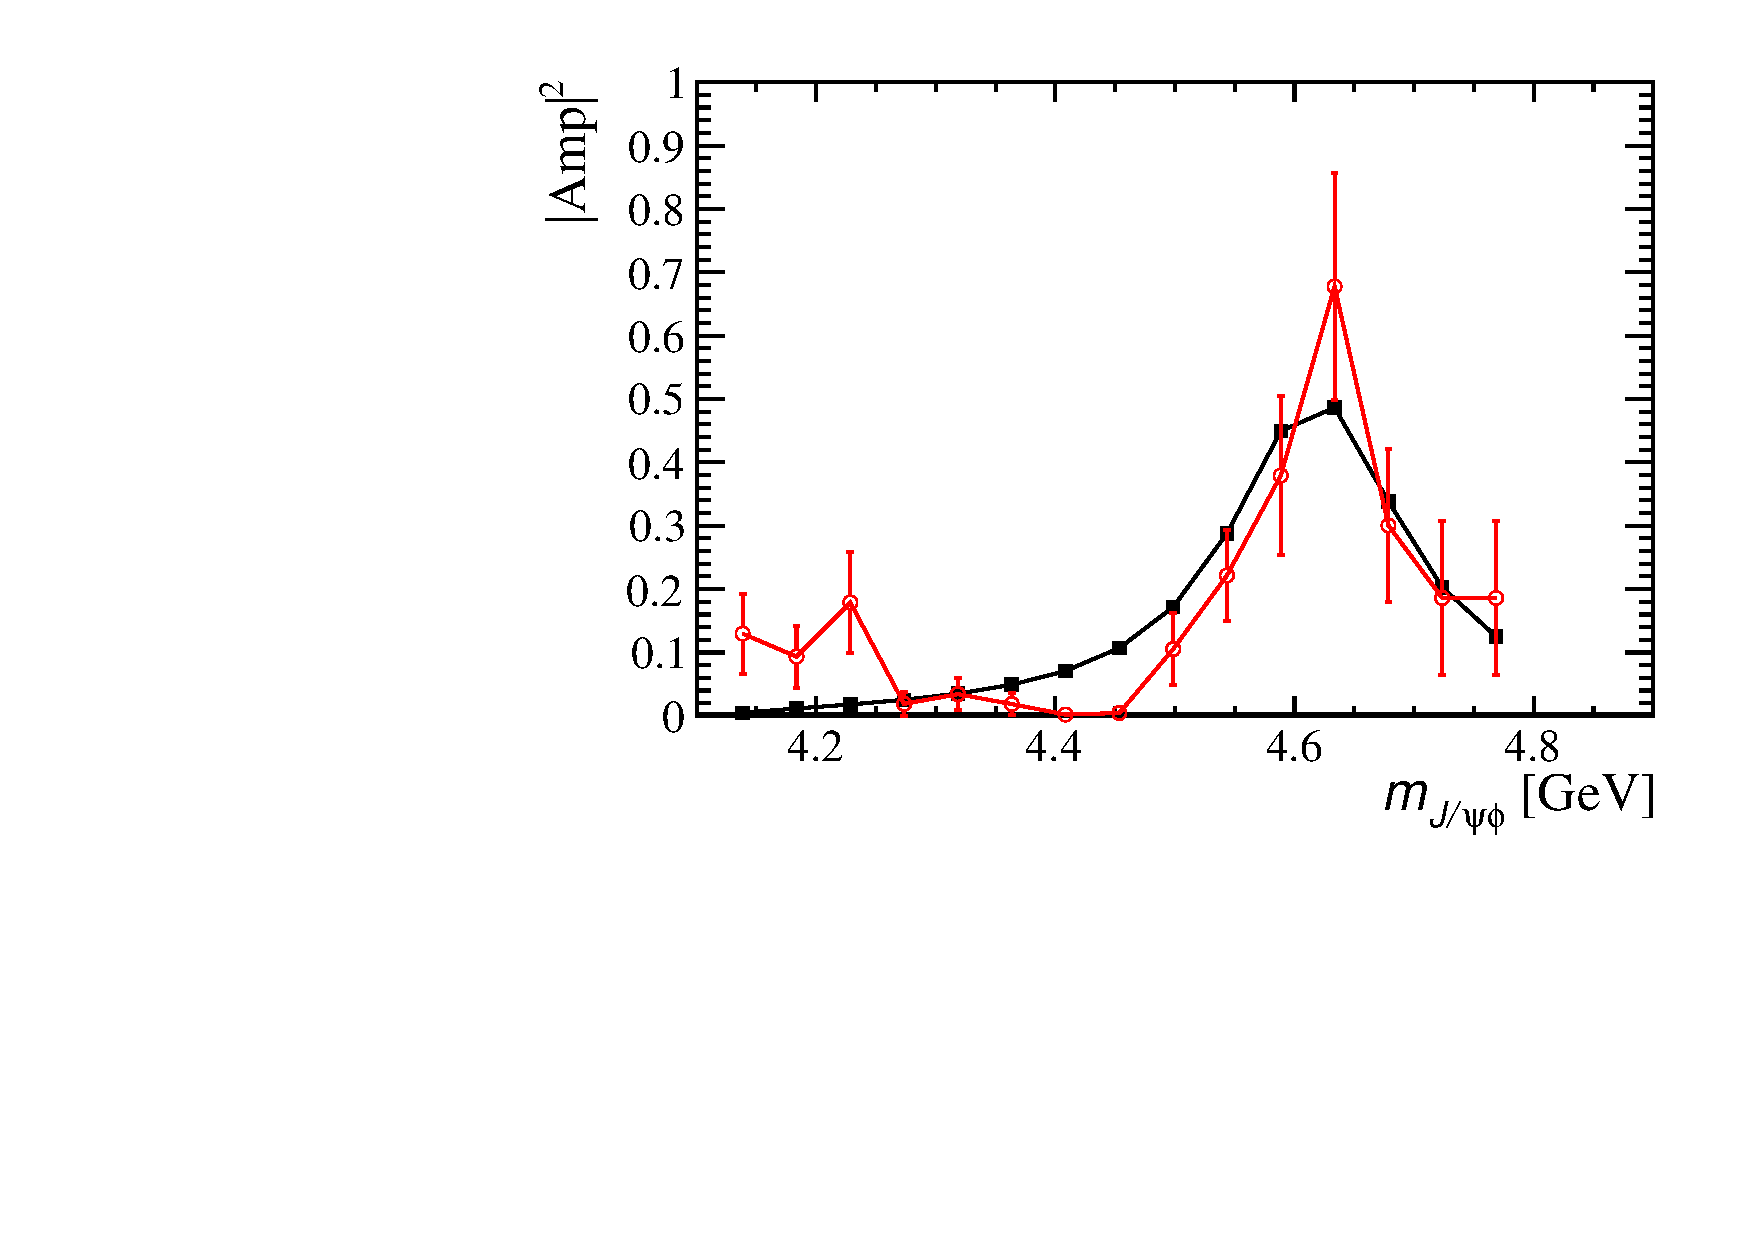
\includegraphics[width=0.4\textwidth]{Figures/03_Zcs/app_MI/A2_X1M}%
\put(-35,105) {\textrm{\small \bf(a)}}%
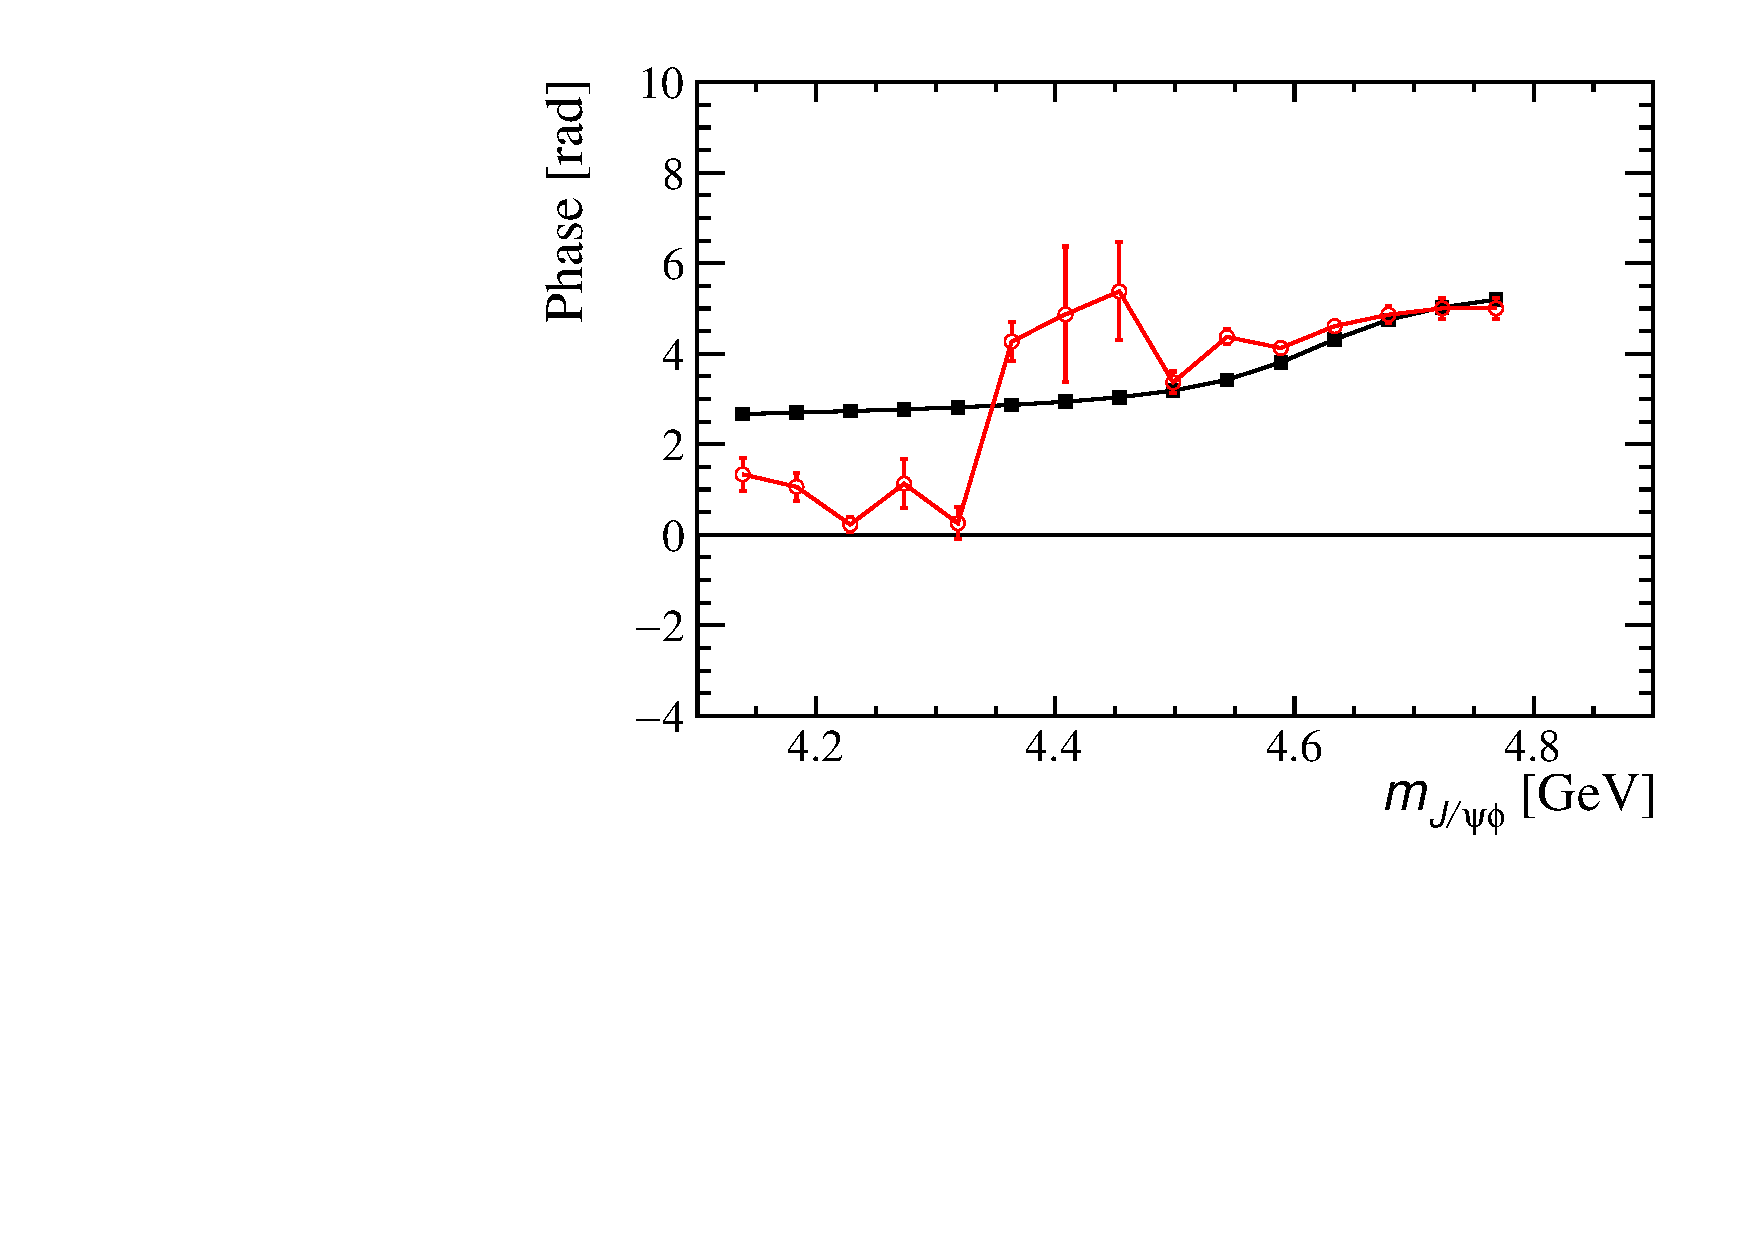
\includegraphics[width=0.4\textwidth]{Figures/03_Zcs/app_MI/Ph_X1M}
\put(-35,105){\textrm{\small \bf(b)}}
\caption{(a) Amplitude squared and (b) phase motion for $1^-$ $X$ wave obtained from the model-independent method (red  open) and the nominal BW-sum fit (black solid).
The BW-sum model has one pole at $M_0-i\Gamma_0/2=4626-i\,174/2$ \mev.}
\label{fig:MIX1M}
\end{figure*}

\begin{figure*}[hbtp]
\centering
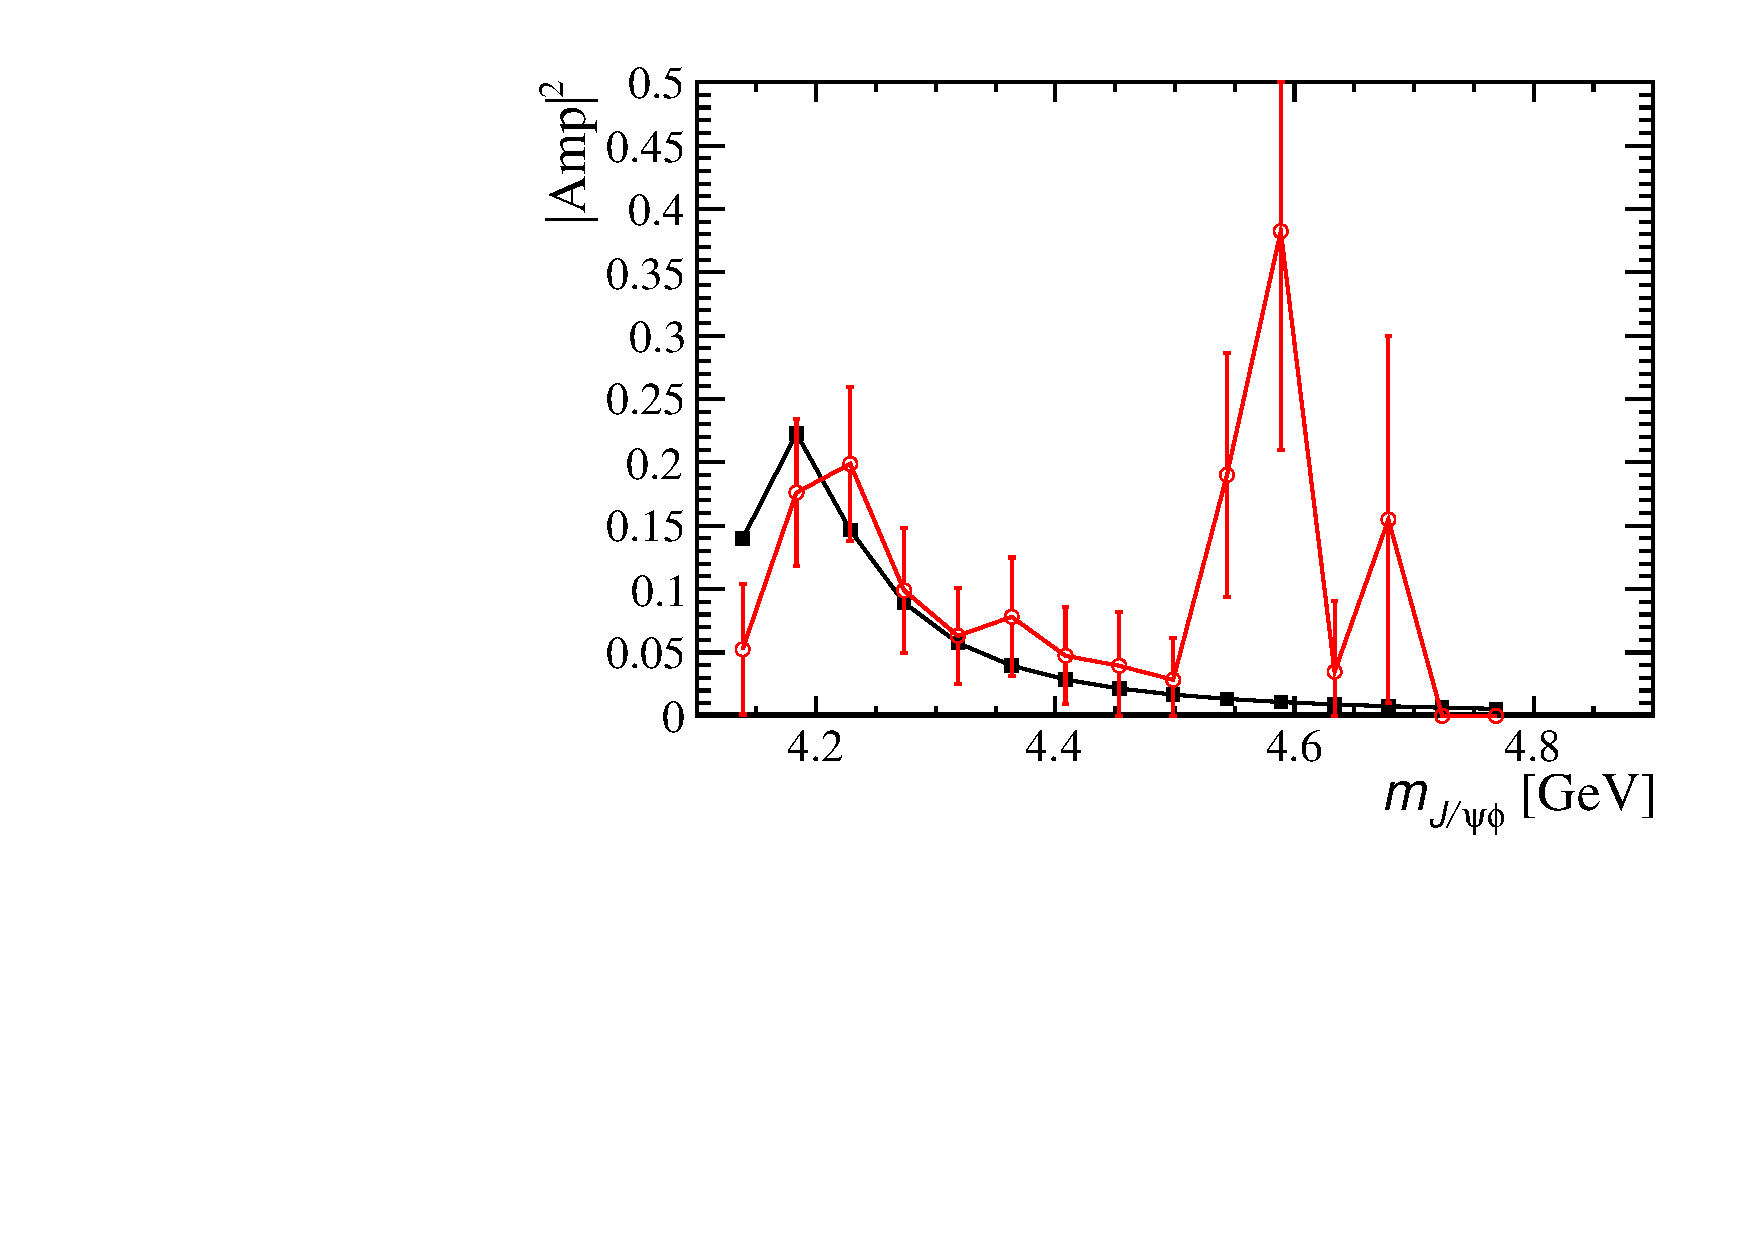
\includegraphics[width=0.4\textwidth]{Figures/03_Zcs/app_MI/A2_X2M}%
\put(-35,105) {\textrm{\small \bf(a)}}%
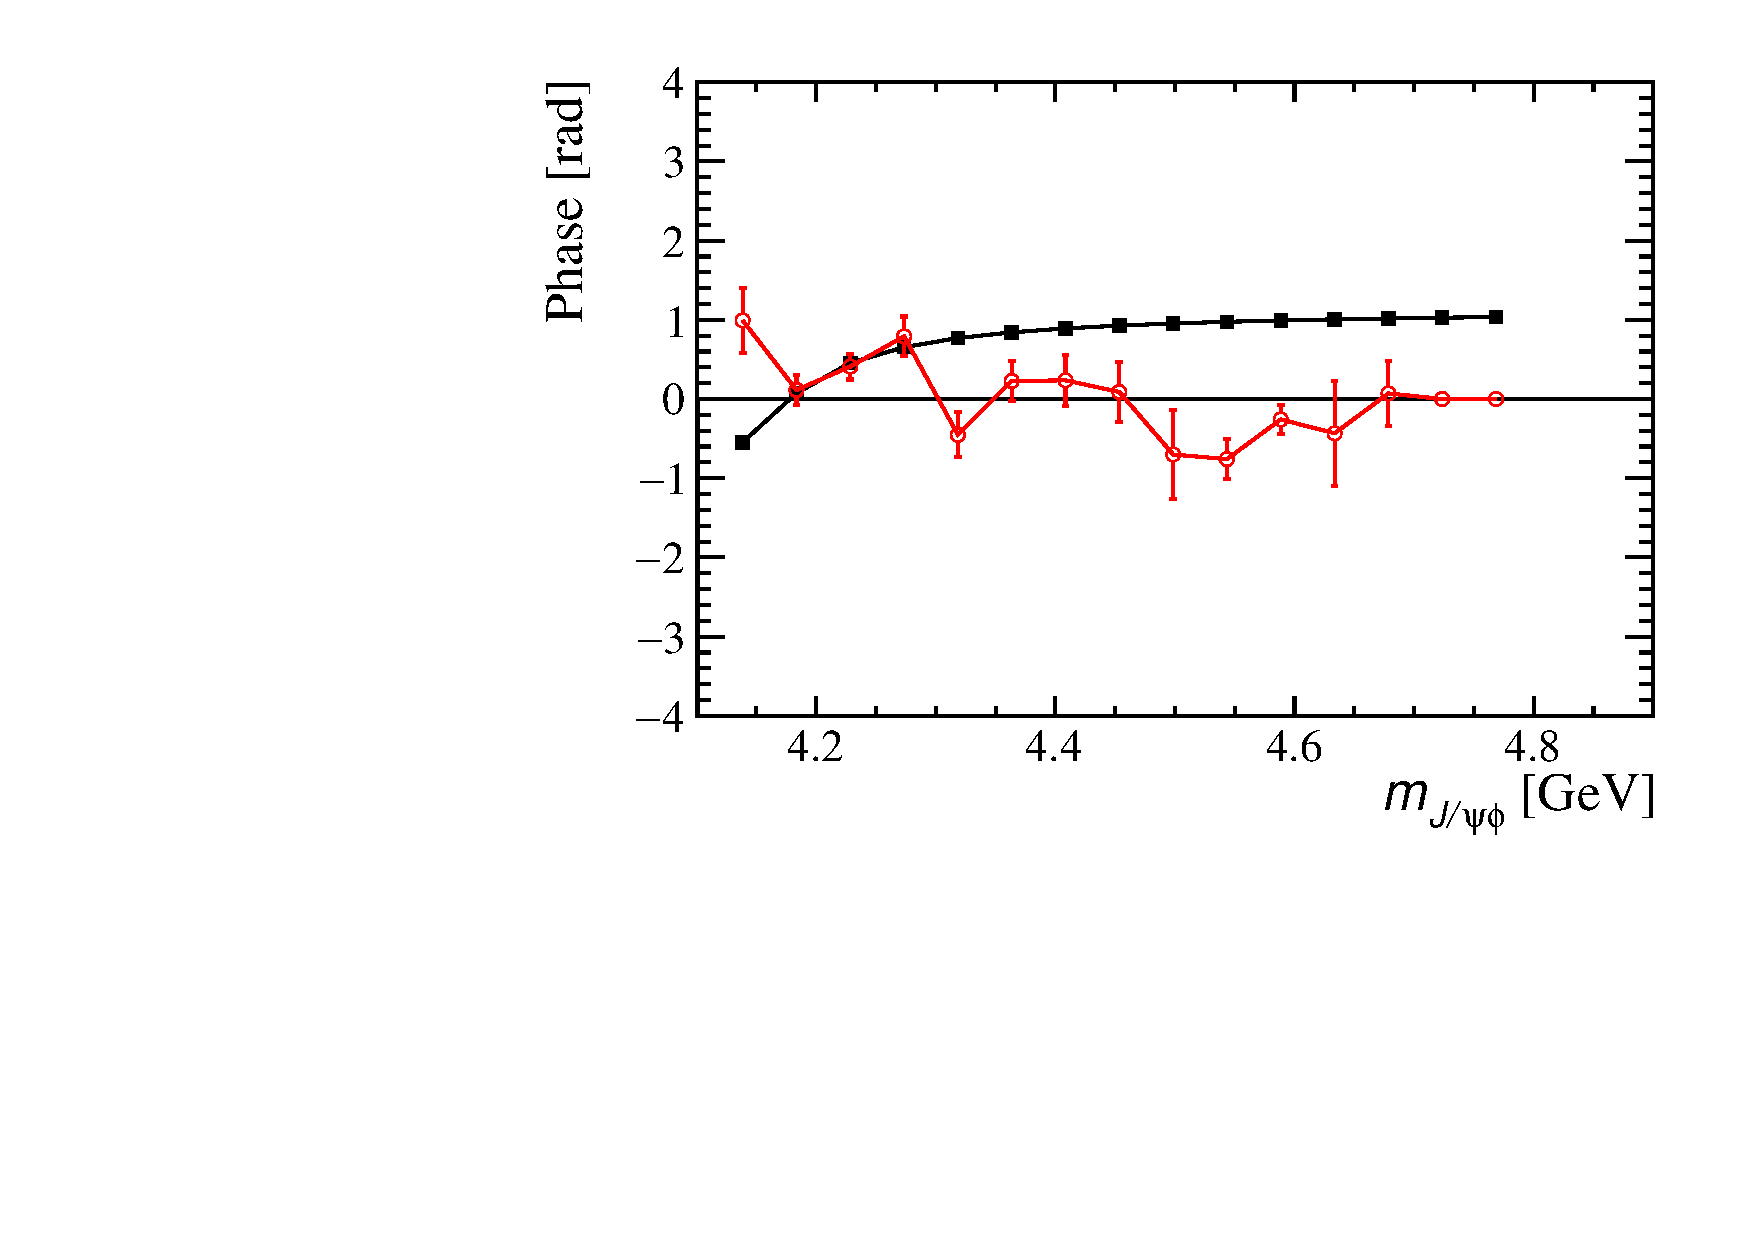
\includegraphics[width=0.4\textwidth]{Figures/03_Zcs/app_MI/Ph_X2M}
\put(-35,105){\textrm{\small \bf(b)}}
\caption{(a) Amplitude squared and (b) phase motion for $2^-$ $X$ wave obtained from the model-independent method (red  open) and the nominal BW-sum fit (black solid).
The BW-sum model has one pole at $M_0-i\Gamma_0/2=4146-i\,135/2$\mev.}
\label{fig:MIX2M}
\end{figure*}

\begin{figure}[hbtp]
\centering
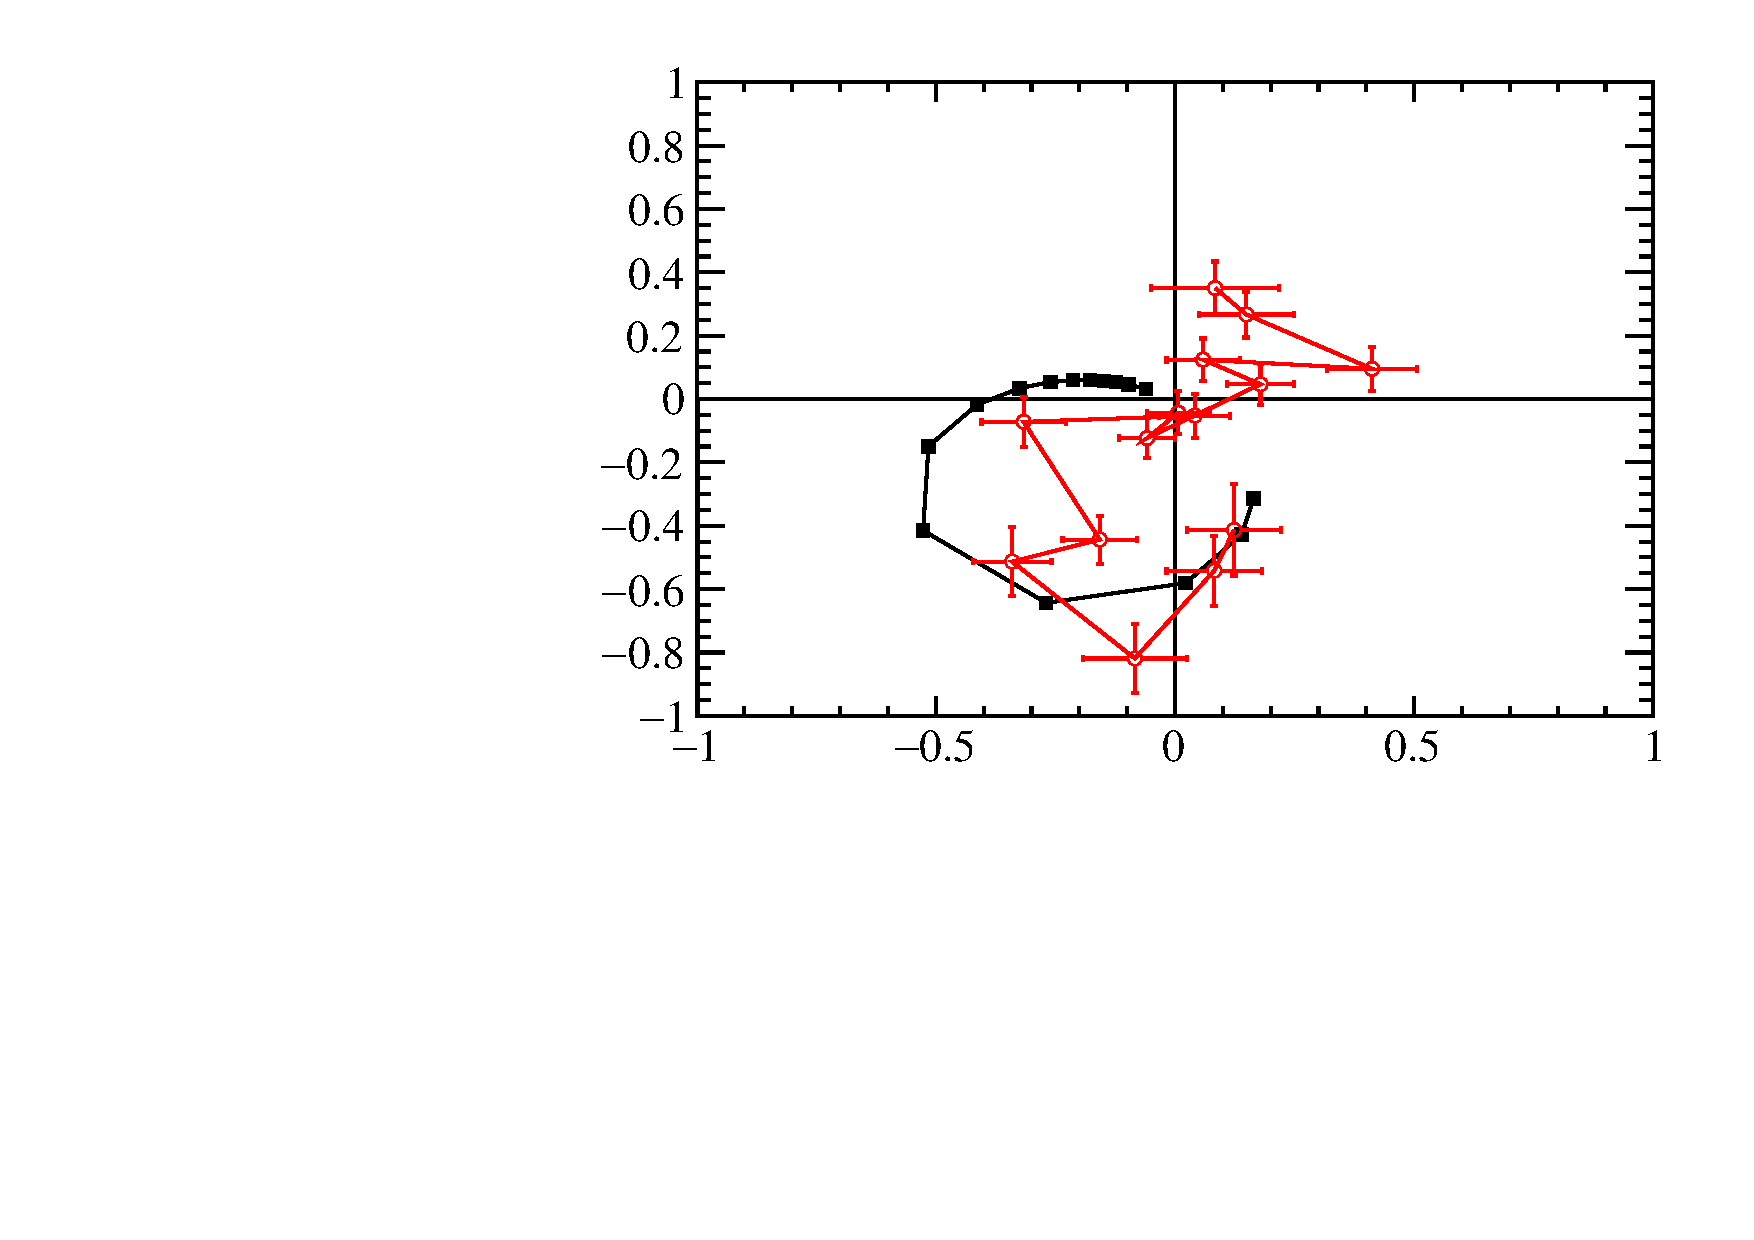
\includegraphics[width=0.4\textwidth]{Figures/03_Zcs/app_MI/Argand_X1M}%
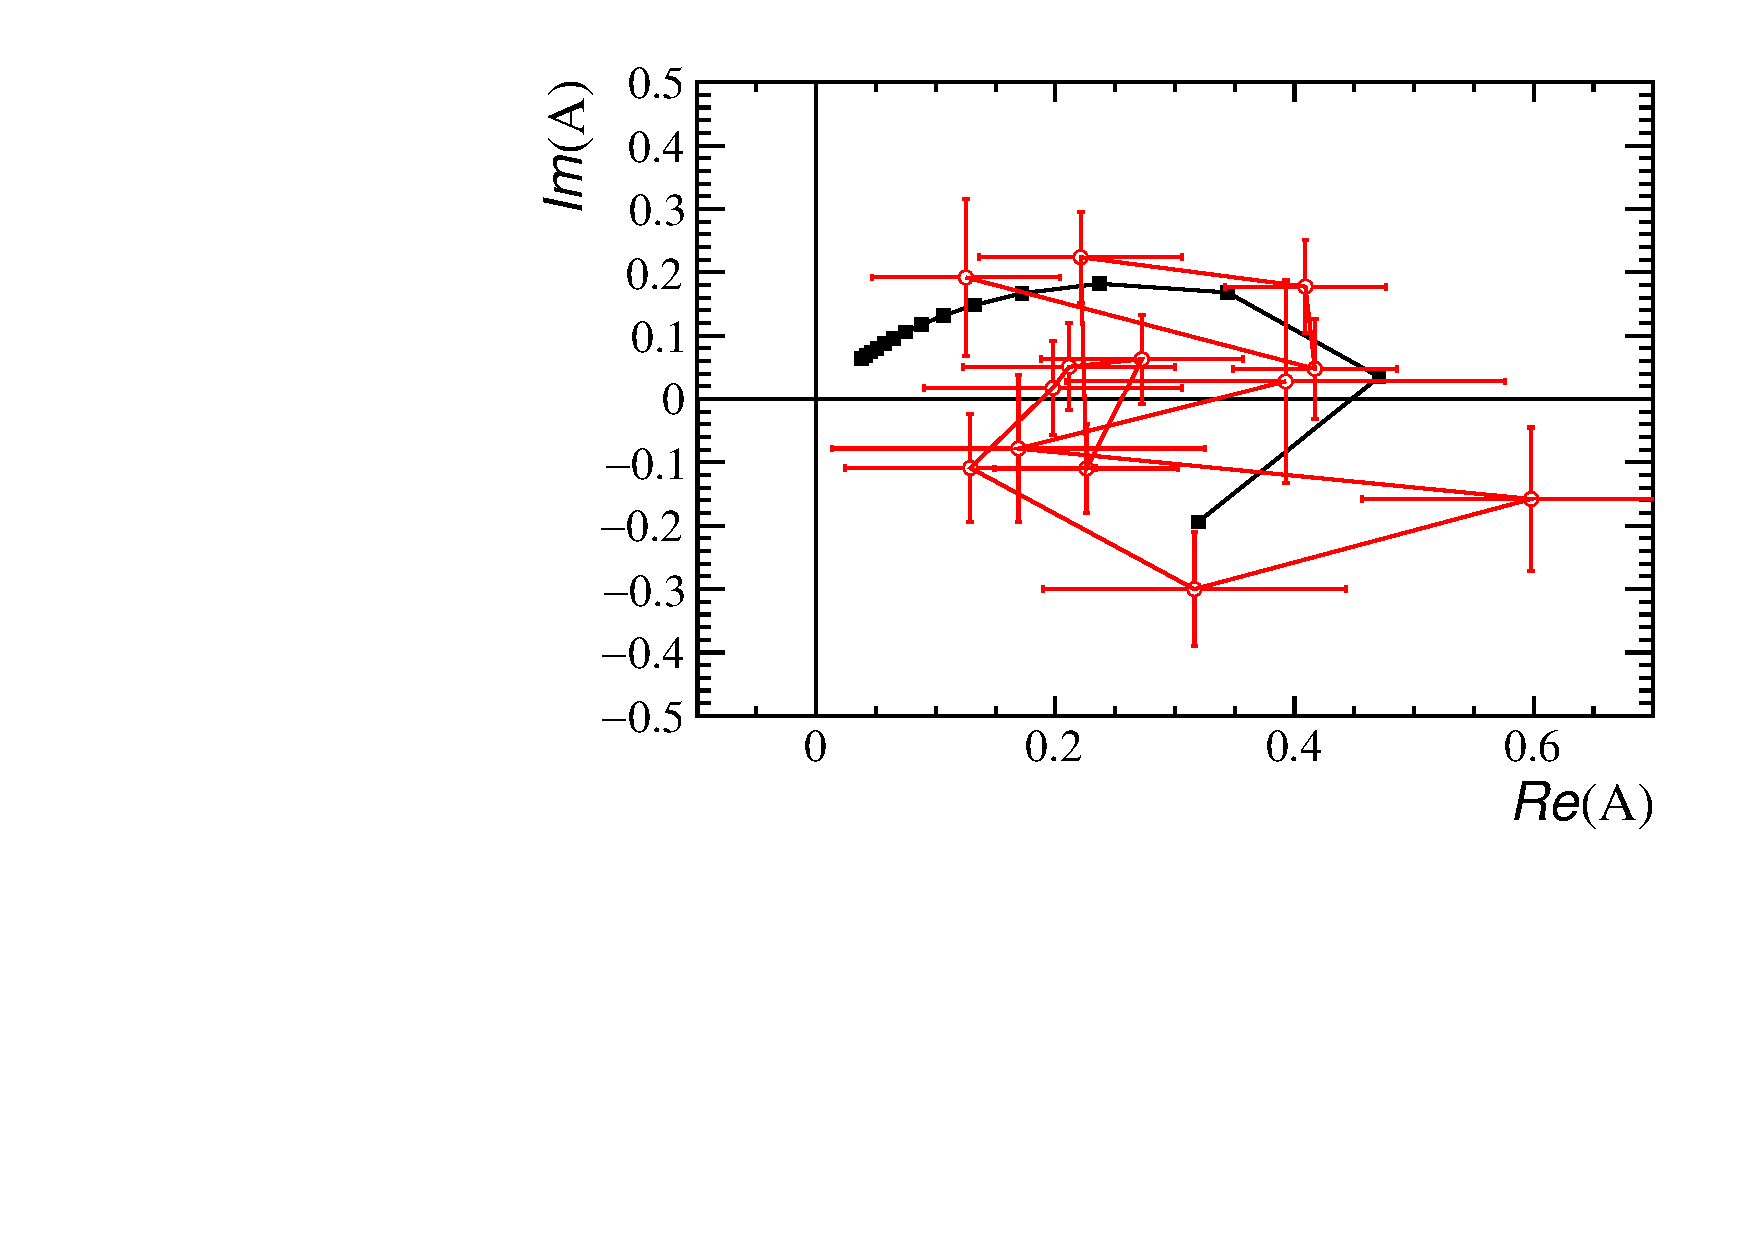
\includegraphics[width=0.4\textwidth]{Figures/03_Zcs/app_MI/Argand_X2M}
\caption{(Left) Argand plot of $1^-$ $X$ waves obtained from the model-independent method (red  open) and the nominal BW-sum fit (black solid). The BW-sum model has poles poles at $M_0-i\Gamma_0/2=4626-i\,174/2$ \mev. (Right) Argand plot of $2-$ $X$ waves obtained from the model-independent method (red  open) and the nominal BW-sum fit (black solid). The BW-sum model has poles poles at $M_0-i\Gamma_0/2=4146-i\,135/2$\mev.}\label{fig:ArgX2}
\end{figure}

Next, we examine $X$ waves, one at a time. 
The amplitude squared and phase motivation of the smallest $L$ wave 
are shown Fig.~\ref{fig:MIX1P} and \ref{fig:MIX0P} for the $1^+$ and $0^+$
~\footnote{The $0^+$ result is obtained without the $Z(4220)$ state, to remove strong negative interference between $0^+$ $X$ and $Z(4220)$ components. 
Otherwise, $Z(4420)$ gets very broad and FF is unphysically large at 150\%.} 
components, respectively. 
The MI results and the nominal BW fit are in good agreement in both magnitude and phase. 
The MI fit confirms the existence of the new $1^+$ $X(4685)$ state at about 4.7\gev, 
in addition to the $X(4140)$ and $X(4274)$ identified in the previous amplitude analysis. 
An amplitude peak is obtained in this region with the phase motion is consistent with the BW fit (Fig.~\ref{fig:MIX1P}). 
The corresponding Argand plots for both waves are shown in Fig.~\ref{fig:ArgX}.  

Next we show the tests for small $X$ contribution of one $J^P$, 
in Figs.~\ref{fig:MIX1M} and \ref{fig:MIX2M} for $1^-$ and $2^-$ $X$ contributions, respectively. 
The MI results also supports activities at of $1^-$ at 4.6\gev and $2^-$ at 4.2\gev found in the sum of BW approach, 
particular for $1^-$ state. 
The corresponding Argand plots for both waves are shown in Fig.~\ref{fig:ArgX2}.

\section{Check on the non-$\phi$ sideband}

The $B^{\pm}$ candidates with $1050<m_{KK}<1100 \mev$  are selected, and referred to as the $\phi$ sideband sample.
The yields of $B\to\jpsi KKK$ signal and of combinatorial background in the $\pm15\mev$ mass range around the peak
are summarized in Table.\ref{table:app_phi_sideband_yields}.

\begin{table}[h]
\begin{center}
\caption{The signal and combinatorial background yields in the $\pm15\mev$ range around the $B$ mass peak
for $B\to\jpsi KKK$ candidates in the $\phi$ sideband (see the text).}
\label{table:app_phi_sideband_yields}
\begin{tabular}{cc}
\hline
 type &  yields \\
\hline
signal & $3766 \pm 73$ \\
combinatorial background & $ 2609 \pm 65$\\
\hline
\end{tabular}
\end{center}
\end{table}


The $m_{\jpsi K}$,$m_{\jpsi \phi}$
 and $m_{\phi K}$ distributions are shown in Fig.\ref{fig:mass_distribution_phi_sideband_2}.
The $m_{\jpsi K}$ distribution for the $m_{\jpsi \phi} \in (4.25,4.35)\mathrm{MeV}$ slice is shown in  Fig.\ref{fig:mjpsik_in_mjpsiphi_strip_2}.
There is no sign of any mass peaking, in particular of $Z(4000)$.
The Dalitz plots in the $\phi$ sideband sample are shown in Fig.\ref{fig:dalitz_plot_phi_sideband}.
The $\jpsi\phi$ mass structures, which are prominent in the $B\to\jpsi\phi K$ sample,
are not present when the $m_{KK}$ is selected in the $\phi$ sideband.

\begin{figure}[!hbtp]
\centering
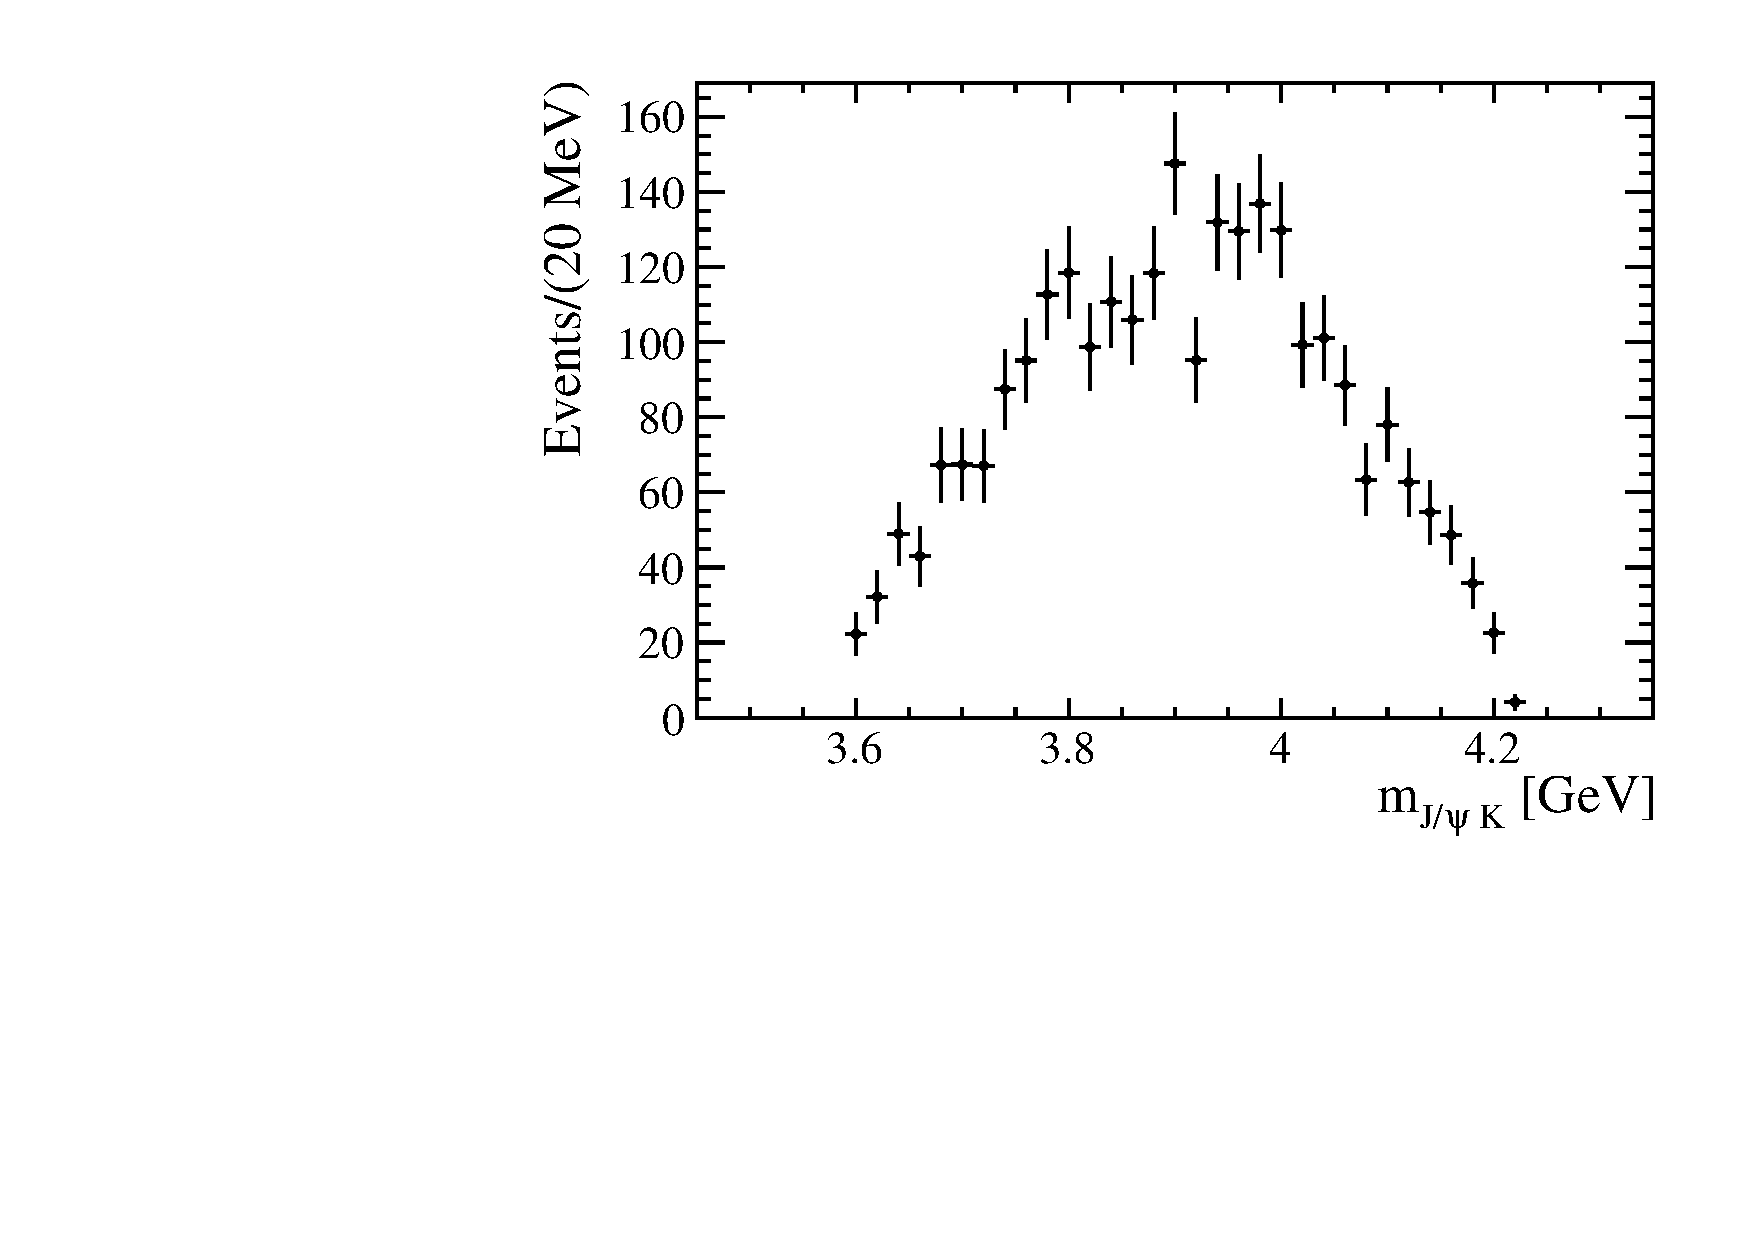
\includegraphics[width=0.33\textwidth]{Figures/03_Zcs/app_non_phi/phi_sideband_mjpsik_1d.pdf}%
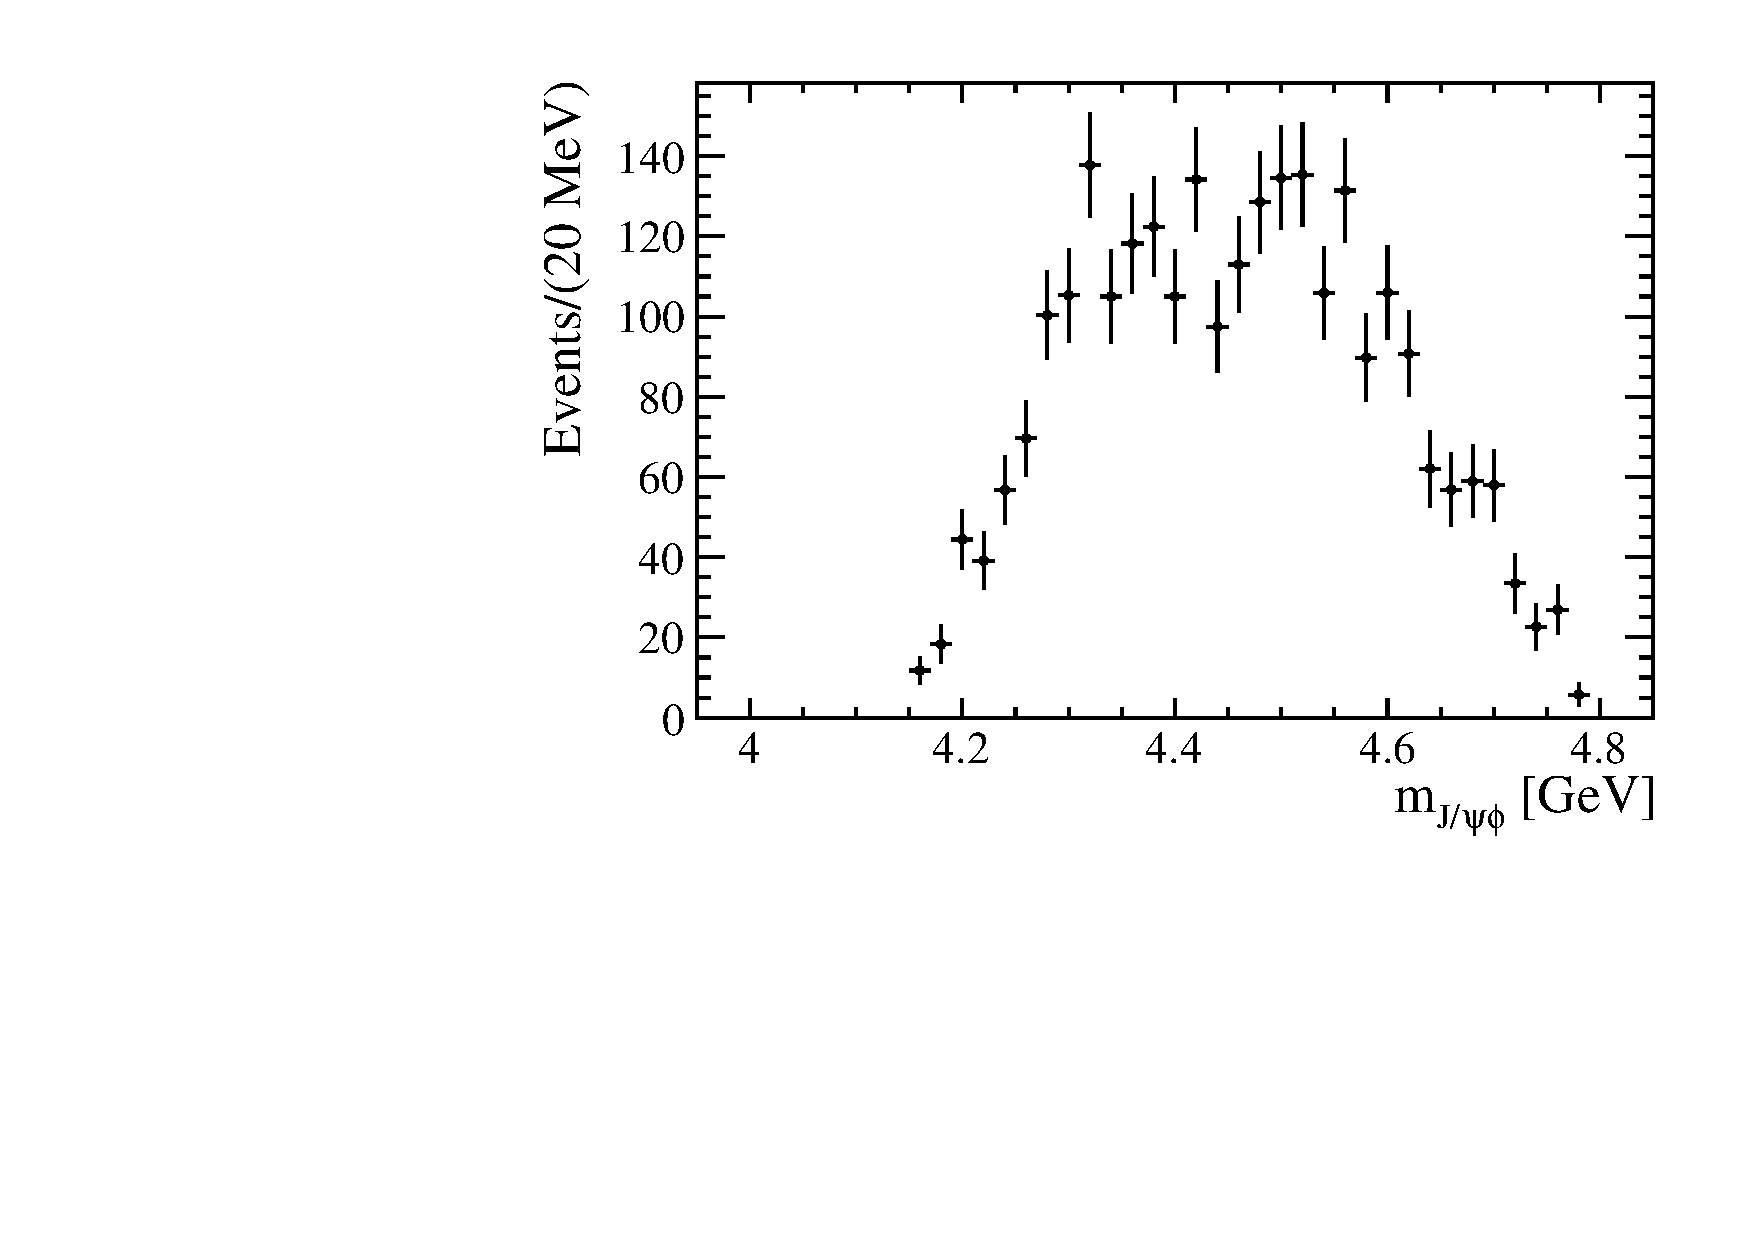
\includegraphics[width=0.33\textwidth]{Figures/03_Zcs/app_non_phi/phi_sideband_mjpsiphi_1d.pdf}
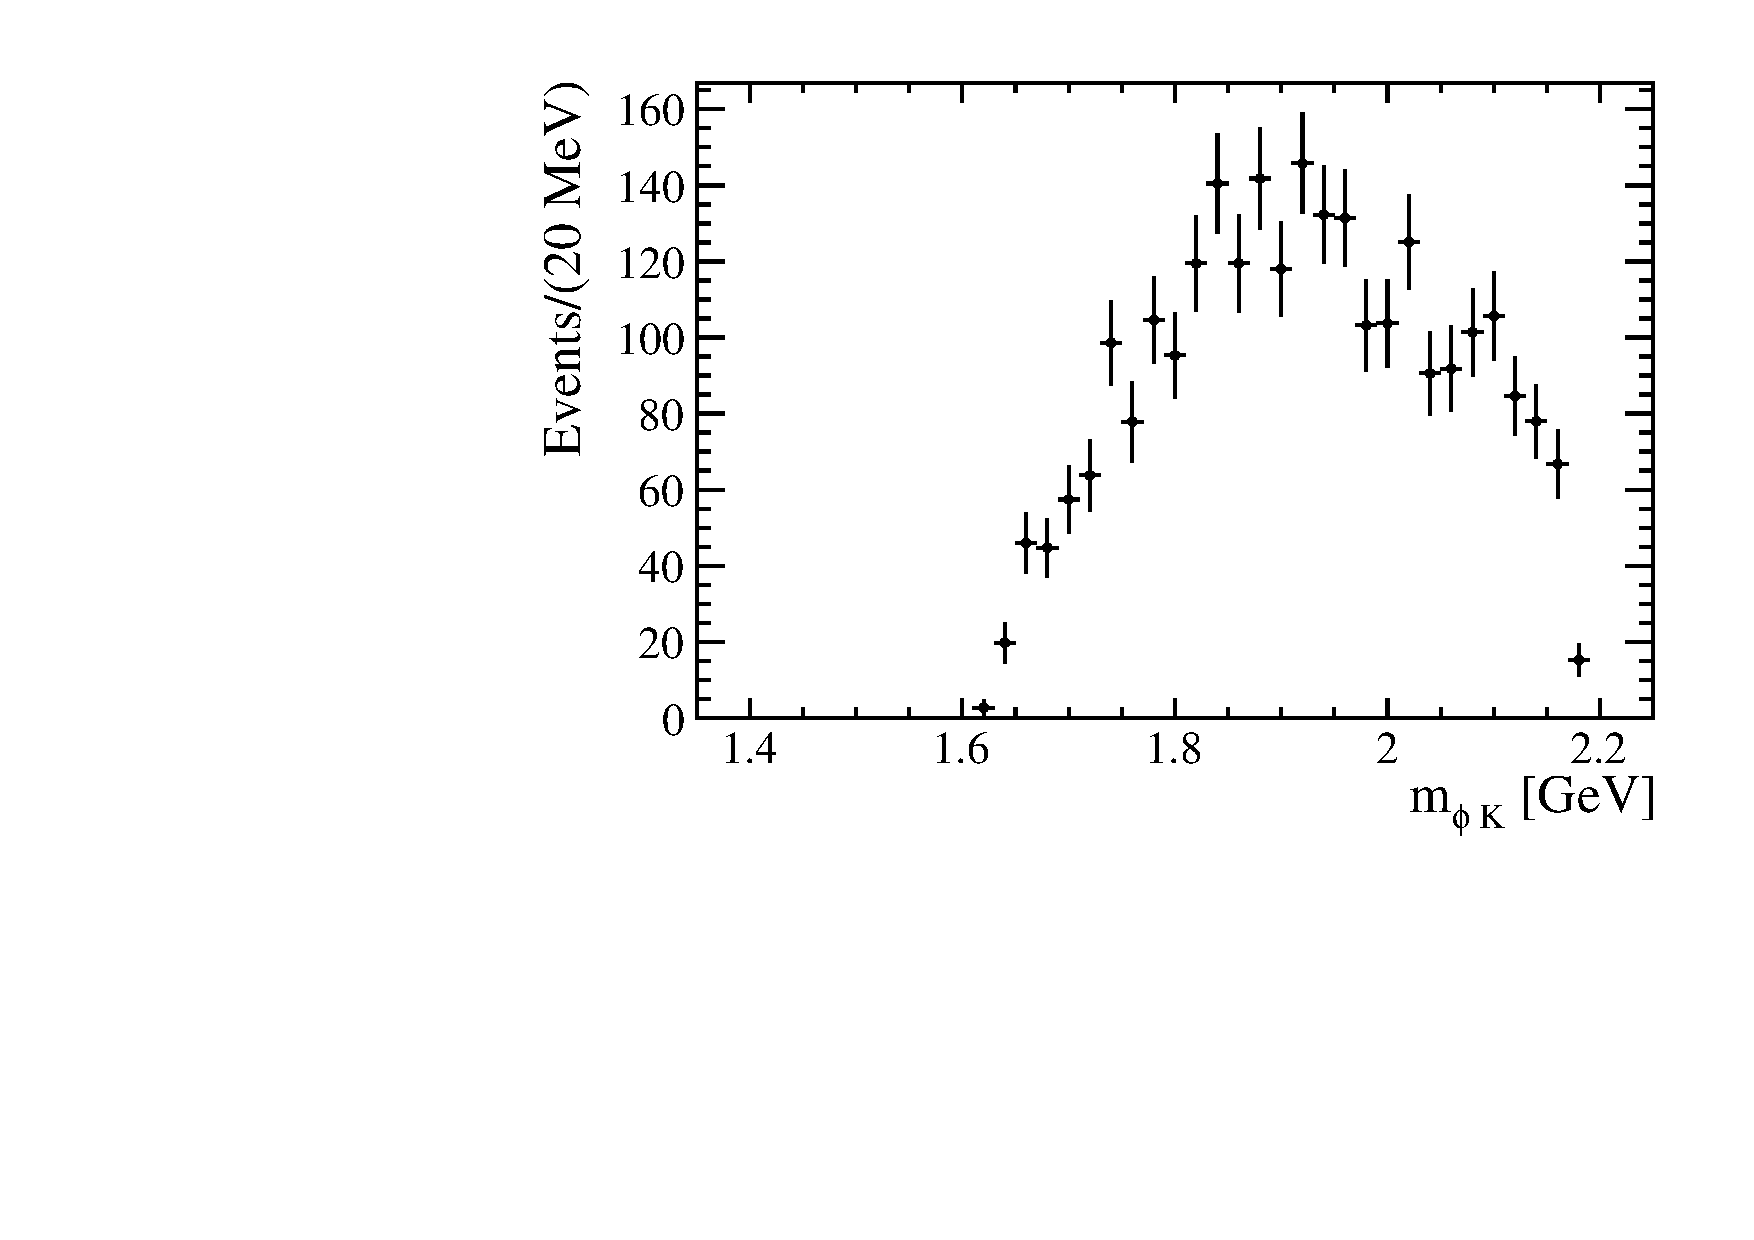
\includegraphics[width=0.33\textwidth]{Figures/03_Zcs/app_non_phi/phi_sideband_mphik_1d.pdf}%
\caption{The mass distribution of $m_{\jpsi K}$,$m_{\jpsi \phi}$
 and $m_{\phi K}$ with phi sideband sample.}
\label{fig:mass_distribution_phi_sideband_2}
\end{figure}

\begin{figure}[!hbtp]
\centering
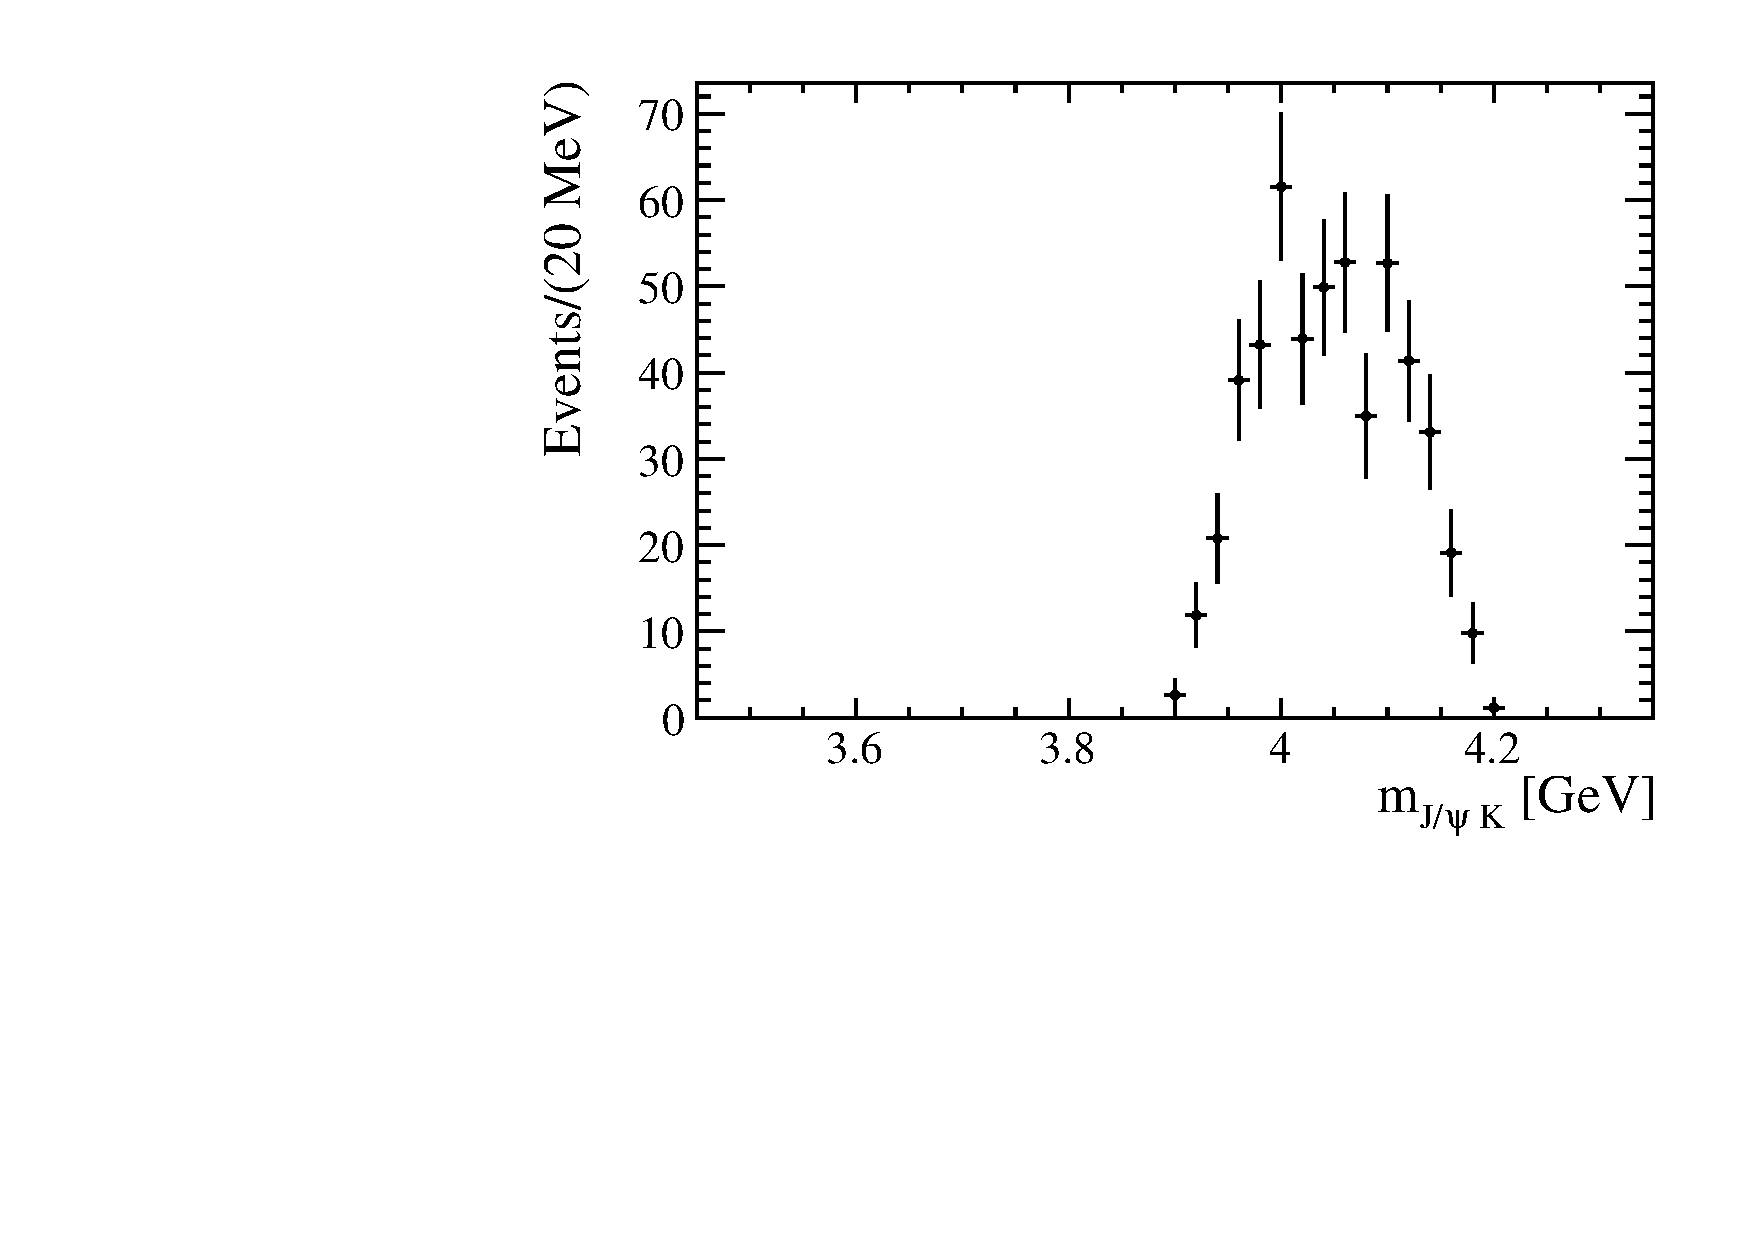
\includegraphics[width=0.4\textwidth]{Figures/03_Zcs/app_non_phi/mjpsik_in_mjpsiphi_strip.pdf}%
\caption{The mass distribution of $m_{\jpsi K}$ with $m_{\jpsi \phi} \in (4.25,4.35)\mev$.}
\label{fig:mjpsik_in_mjpsiphi_strip_2}
\end{figure}


\begin{figure}[!hbtp]
\centering
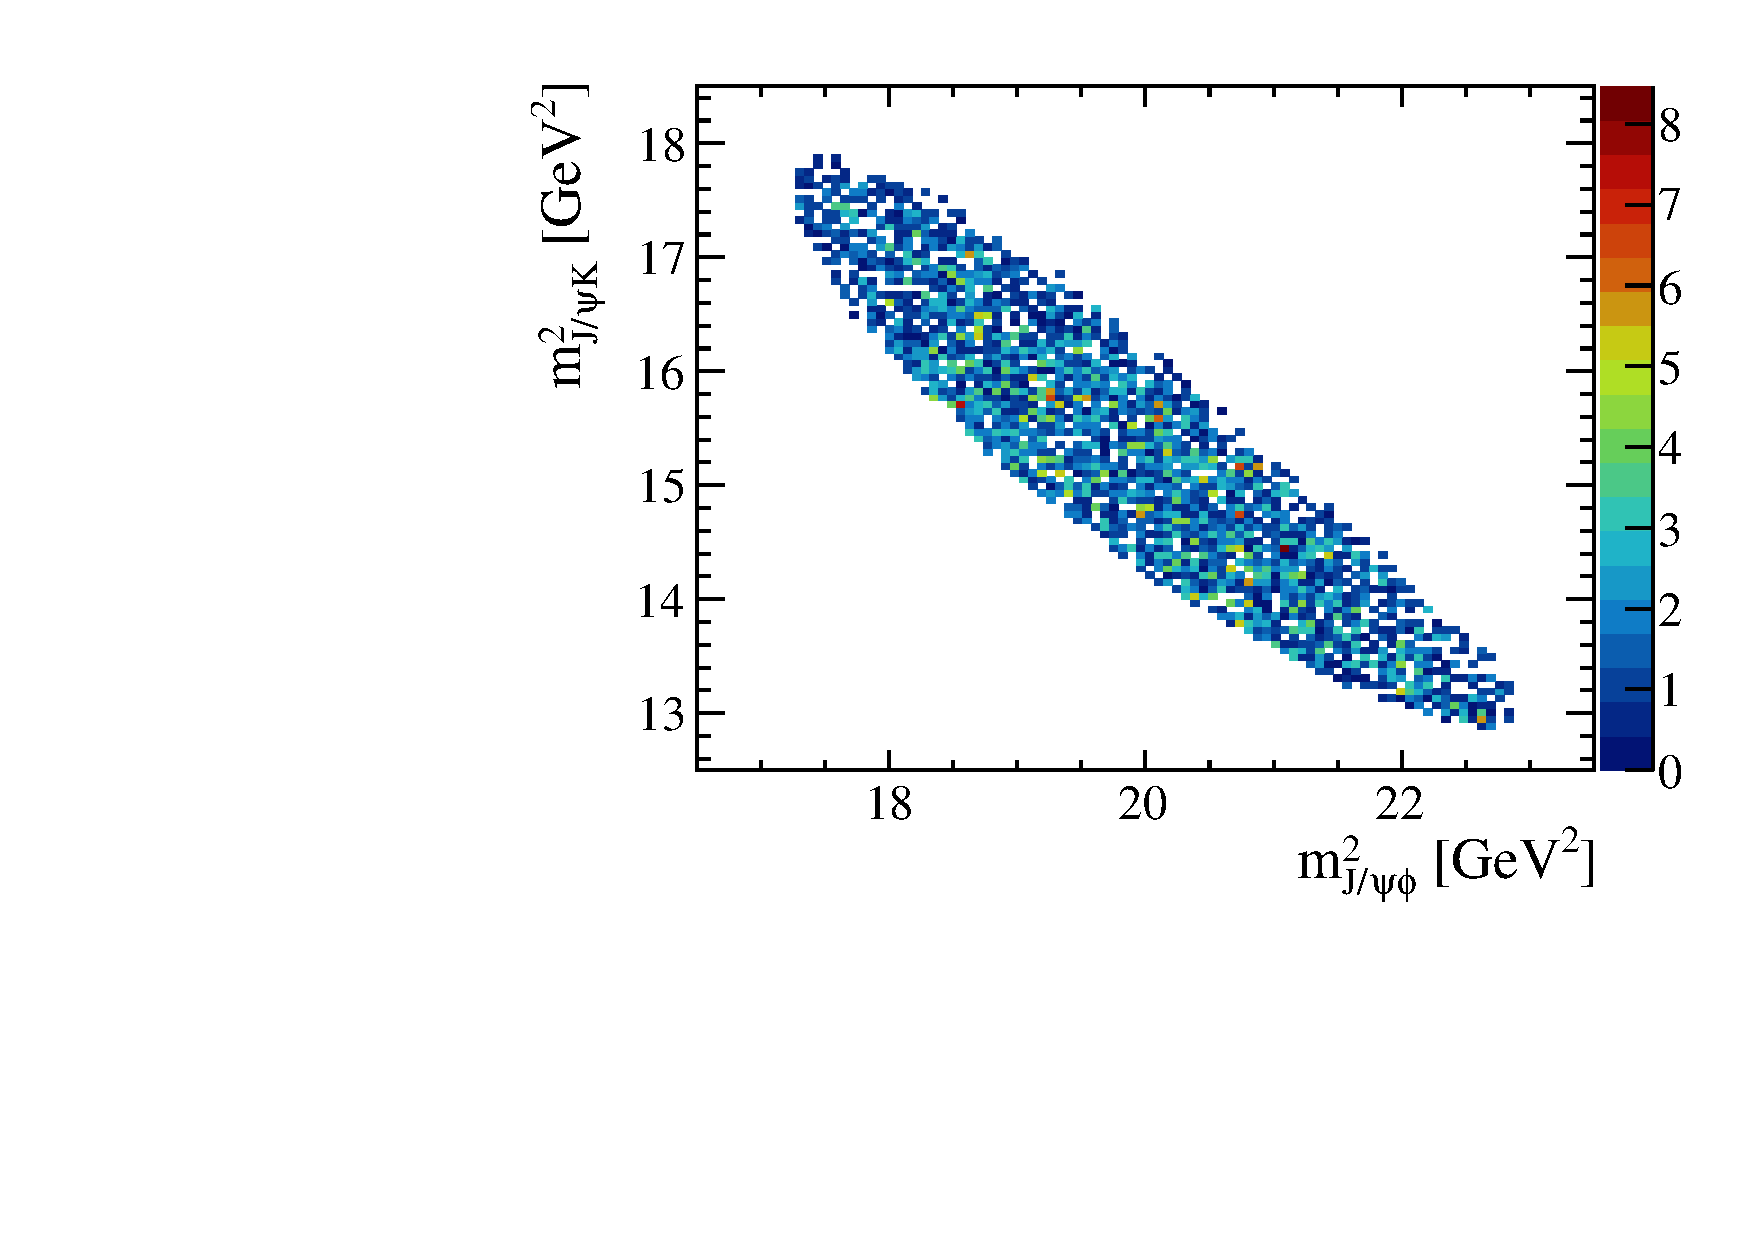
\includegraphics[width=0.33\textwidth]{Figures/03_Zcs/app_non_phi/phi_sideband_mjpsik2_mjpsiphi2.pdf}%
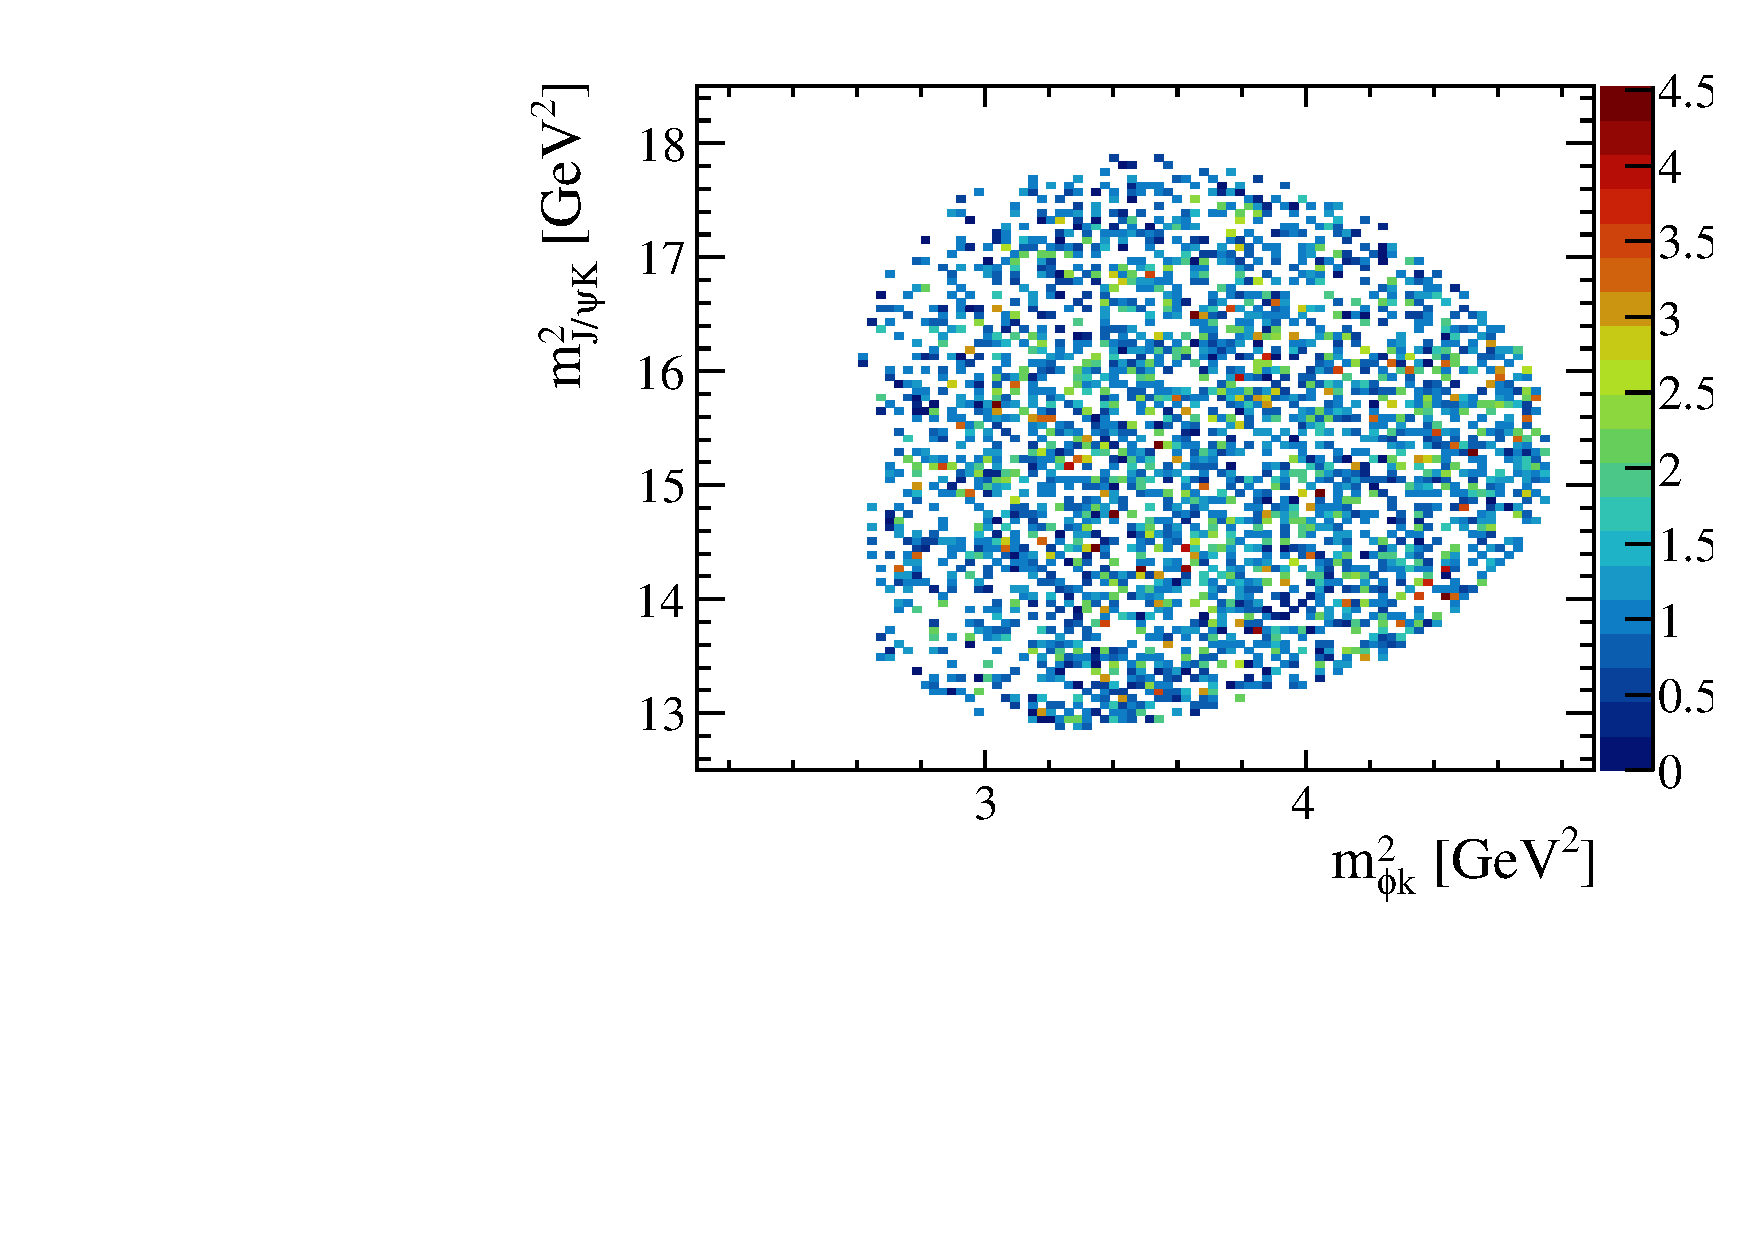
\includegraphics[width=0.33\textwidth]{Figures/03_Zcs/app_non_phi/phi_sideband_mjpsik2_mphik2.pdf}
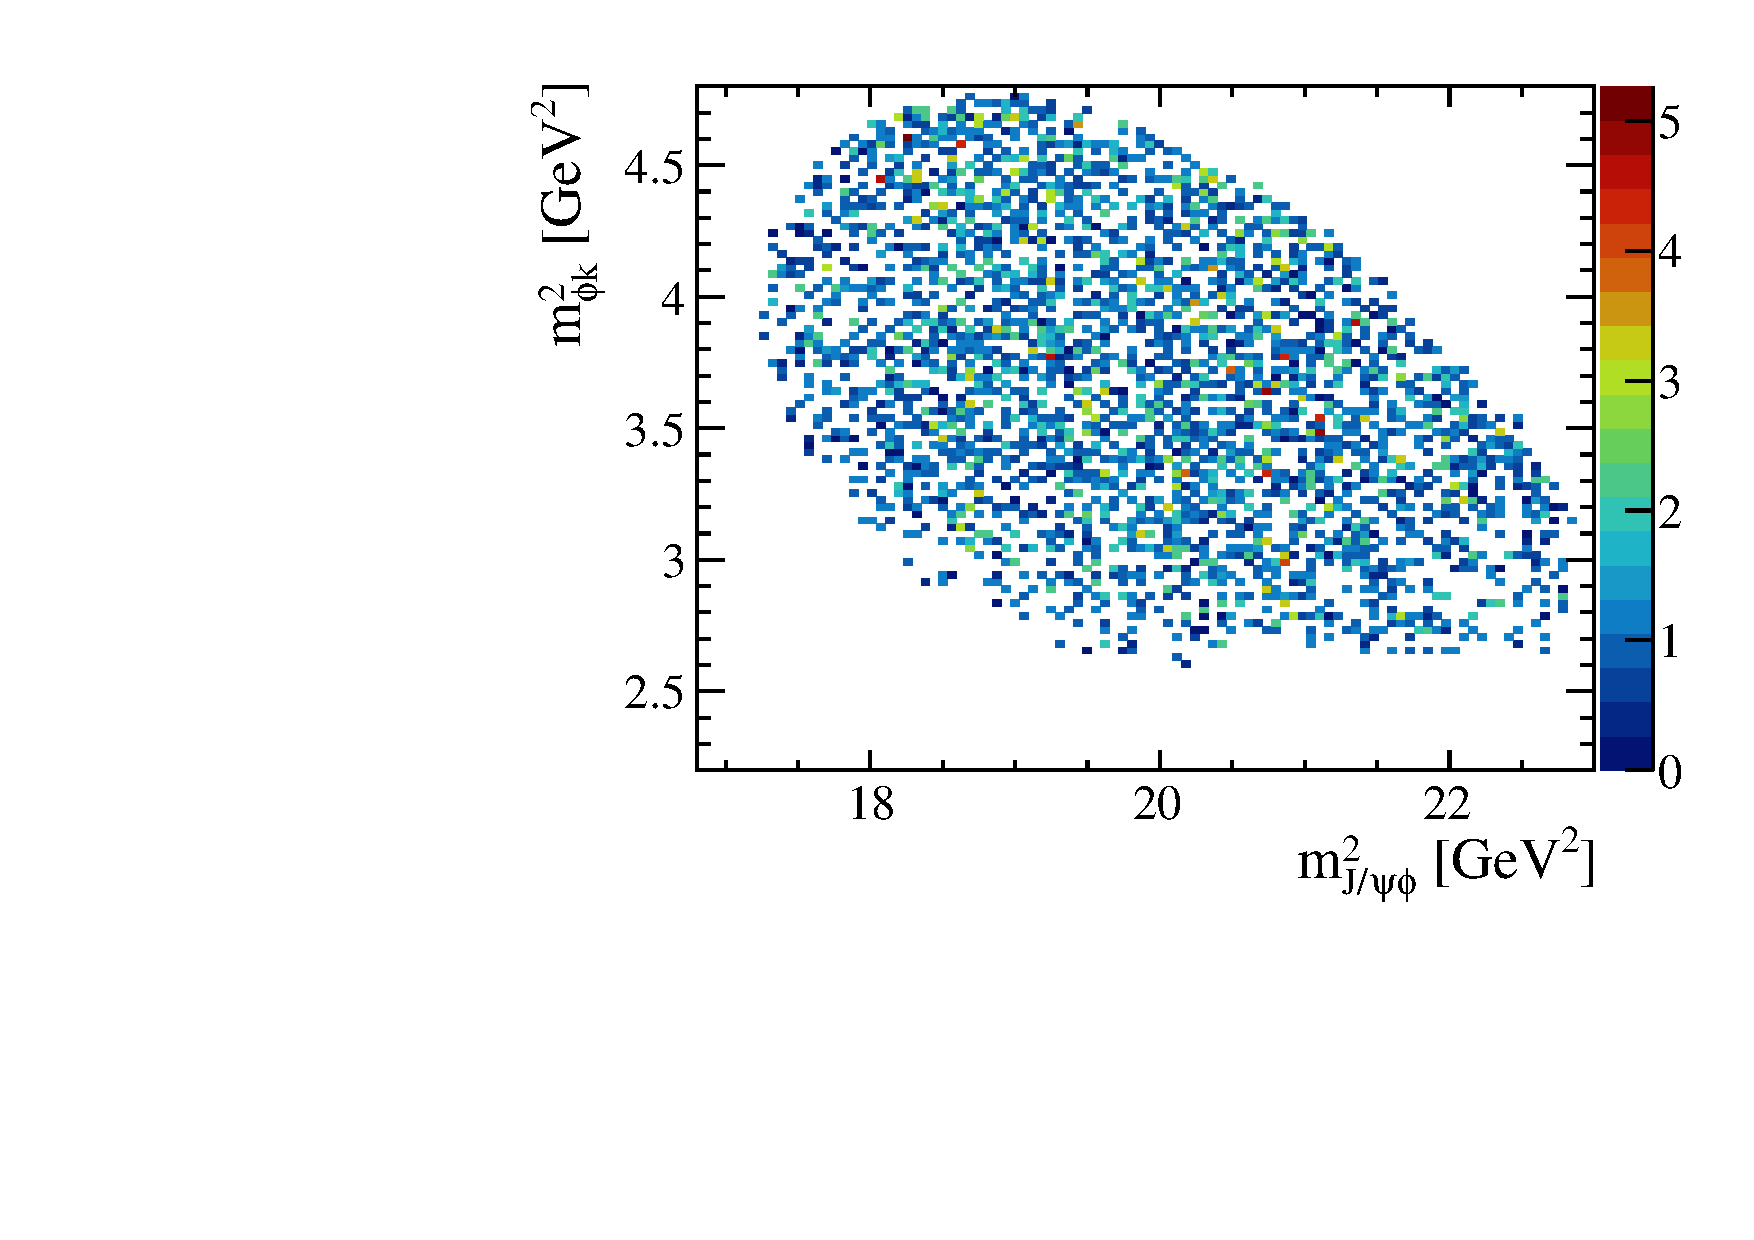
\includegraphics[width=0.33\textwidth]{Figures/03_Zcs/app_non_phi/phi_sideband_mphik2_mjpsiphi2.pdf}%
\caption{The dalitz plot with phi sideband sample.}
\label{fig:dalitz_plot_phi_sideband}
\end{figure}



\section{Kmatix model}
\label{SUPPsec:kmatrix}
Since many $K^*$ resonances with the same $J^P$ are overlapping ($1^+$, $1^-$ and $2^-$ waves), 
the BW sum may not be their best representation. As an alternative, 
we use a simplified K-Matrix formula to describe them. 
The ${\rm BW}(m_{K\phi} | M_{0}^{K^*_n}, \Gamma_{0}^{K^*_n} )$ term in Eq.~(\ref{SUPeq:resshape}) is replaced by: 
\begin{equation}
RKM_{n}(m | M_{0n}, \Gamma_{0n} ) = \frac{\frac{1}{M_{0n}^2-m^2}}{1-i(\sum_j\frac{M_{0j}\Gamma_{0j}(m)}{M_{0j}^2-m^2}+f_{sc}\cdot\rho(m))},
\label{eq:RKM}
\end{equation}
where the denominator sums over the same $J^P$ $K^*$ resonances, and $f_{sc}$ accounts for a possible non-resonance contribution, 
phase space factor $\rho(m)=2p/m$. 
For the non-resonance function, 
if including it, 
$f_{sc}$ is a free parameter in the fit, 
and the numerator in Eq.~(\ref{eq:RKM}) is 1 instead of $1/(M_{0n}^2-m^2)$. 
Here we set $f_{sc}=0$, 
as the non-resonances are modelled by tail of lower mass $K^*$'s.

We use the same $K^*$ resonant masses and widths as those used in the nominal fit. 
The conclusions for the exotic states are unchanged, 
and the results are taken as the systematic uncertainty. 
The projections of this fit onto masses are shown in Fig.~\ref{fig:fitKM}.

\begin{figure}[!tbp]
\centering
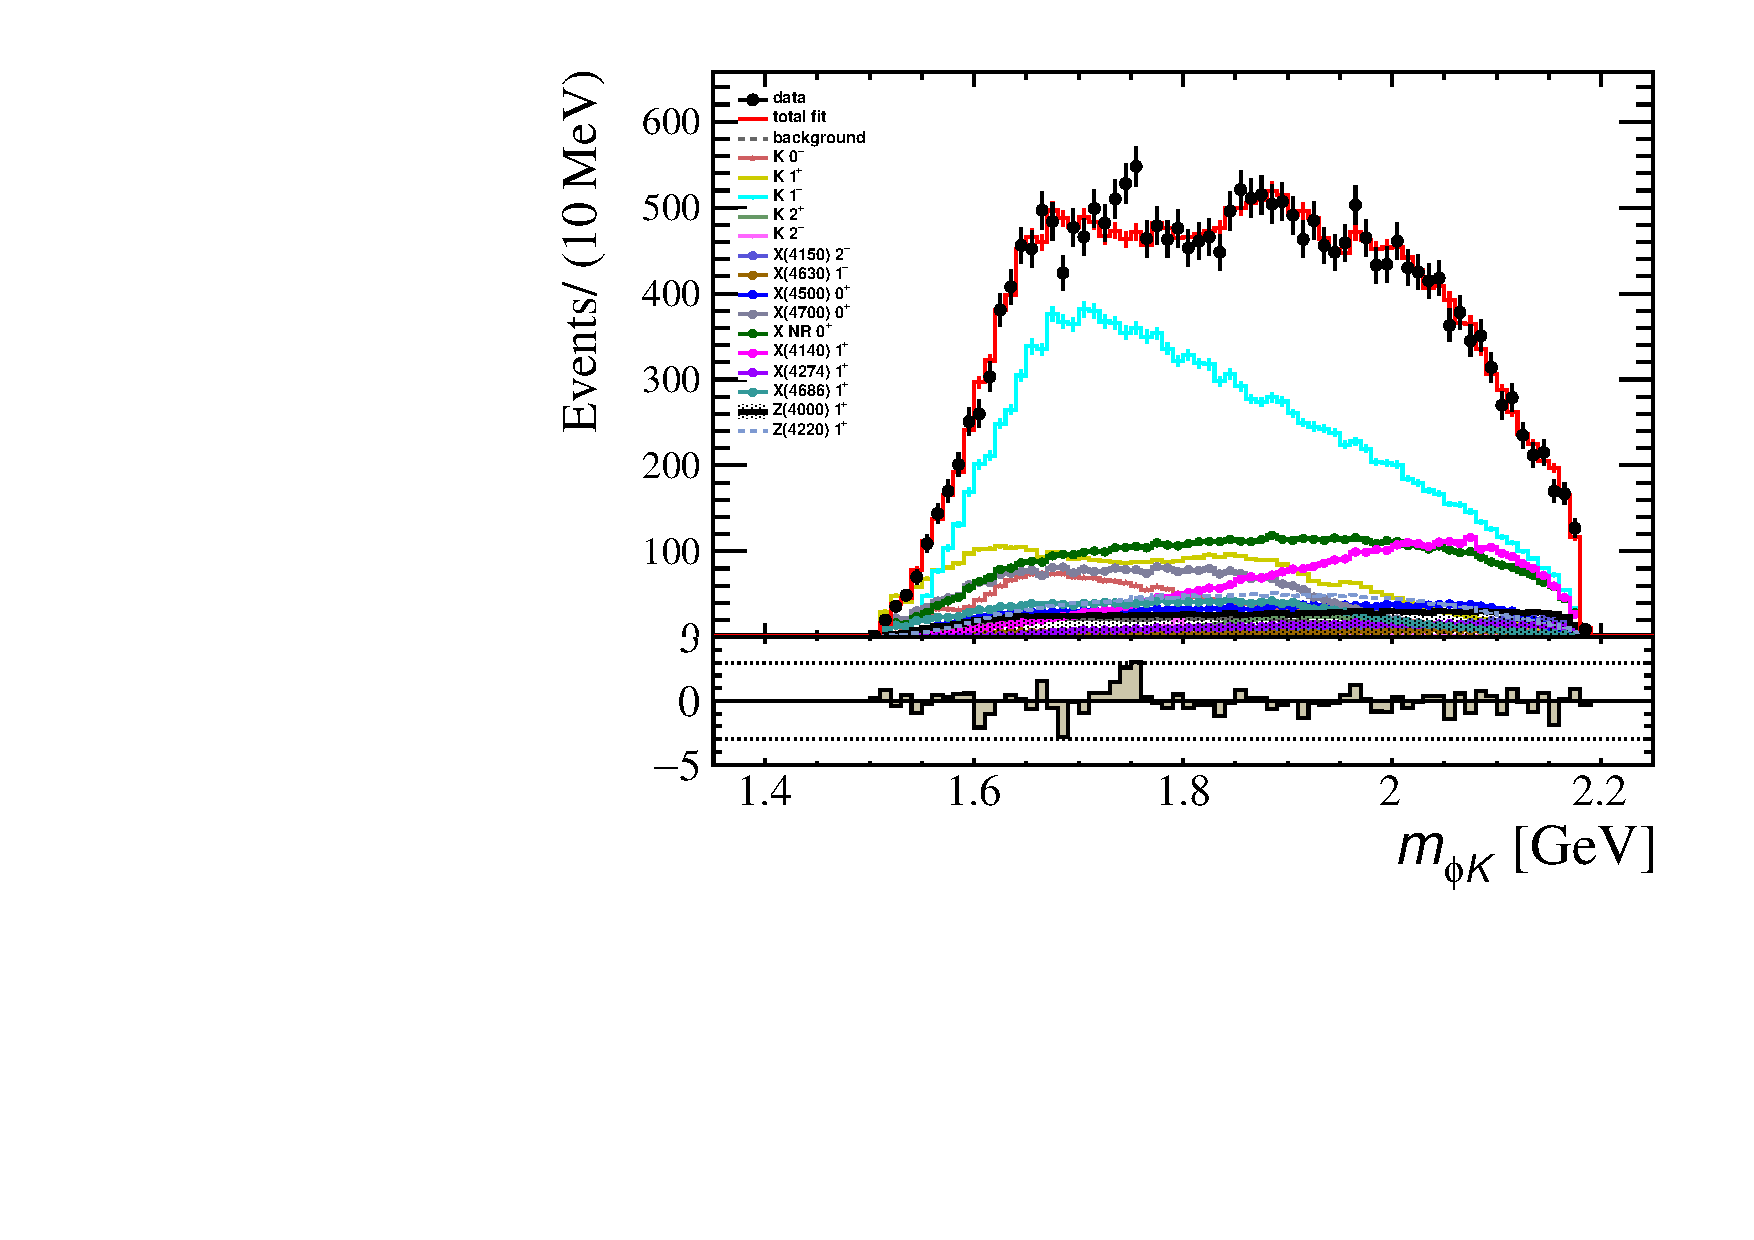
\includegraphics[width=0.33\textwidth]{Figures/03_Zcs/app_Kmatrix/mphik-X2mZ1PKM}
\put(-40,95) {\textrm{\small \bf(a)}}
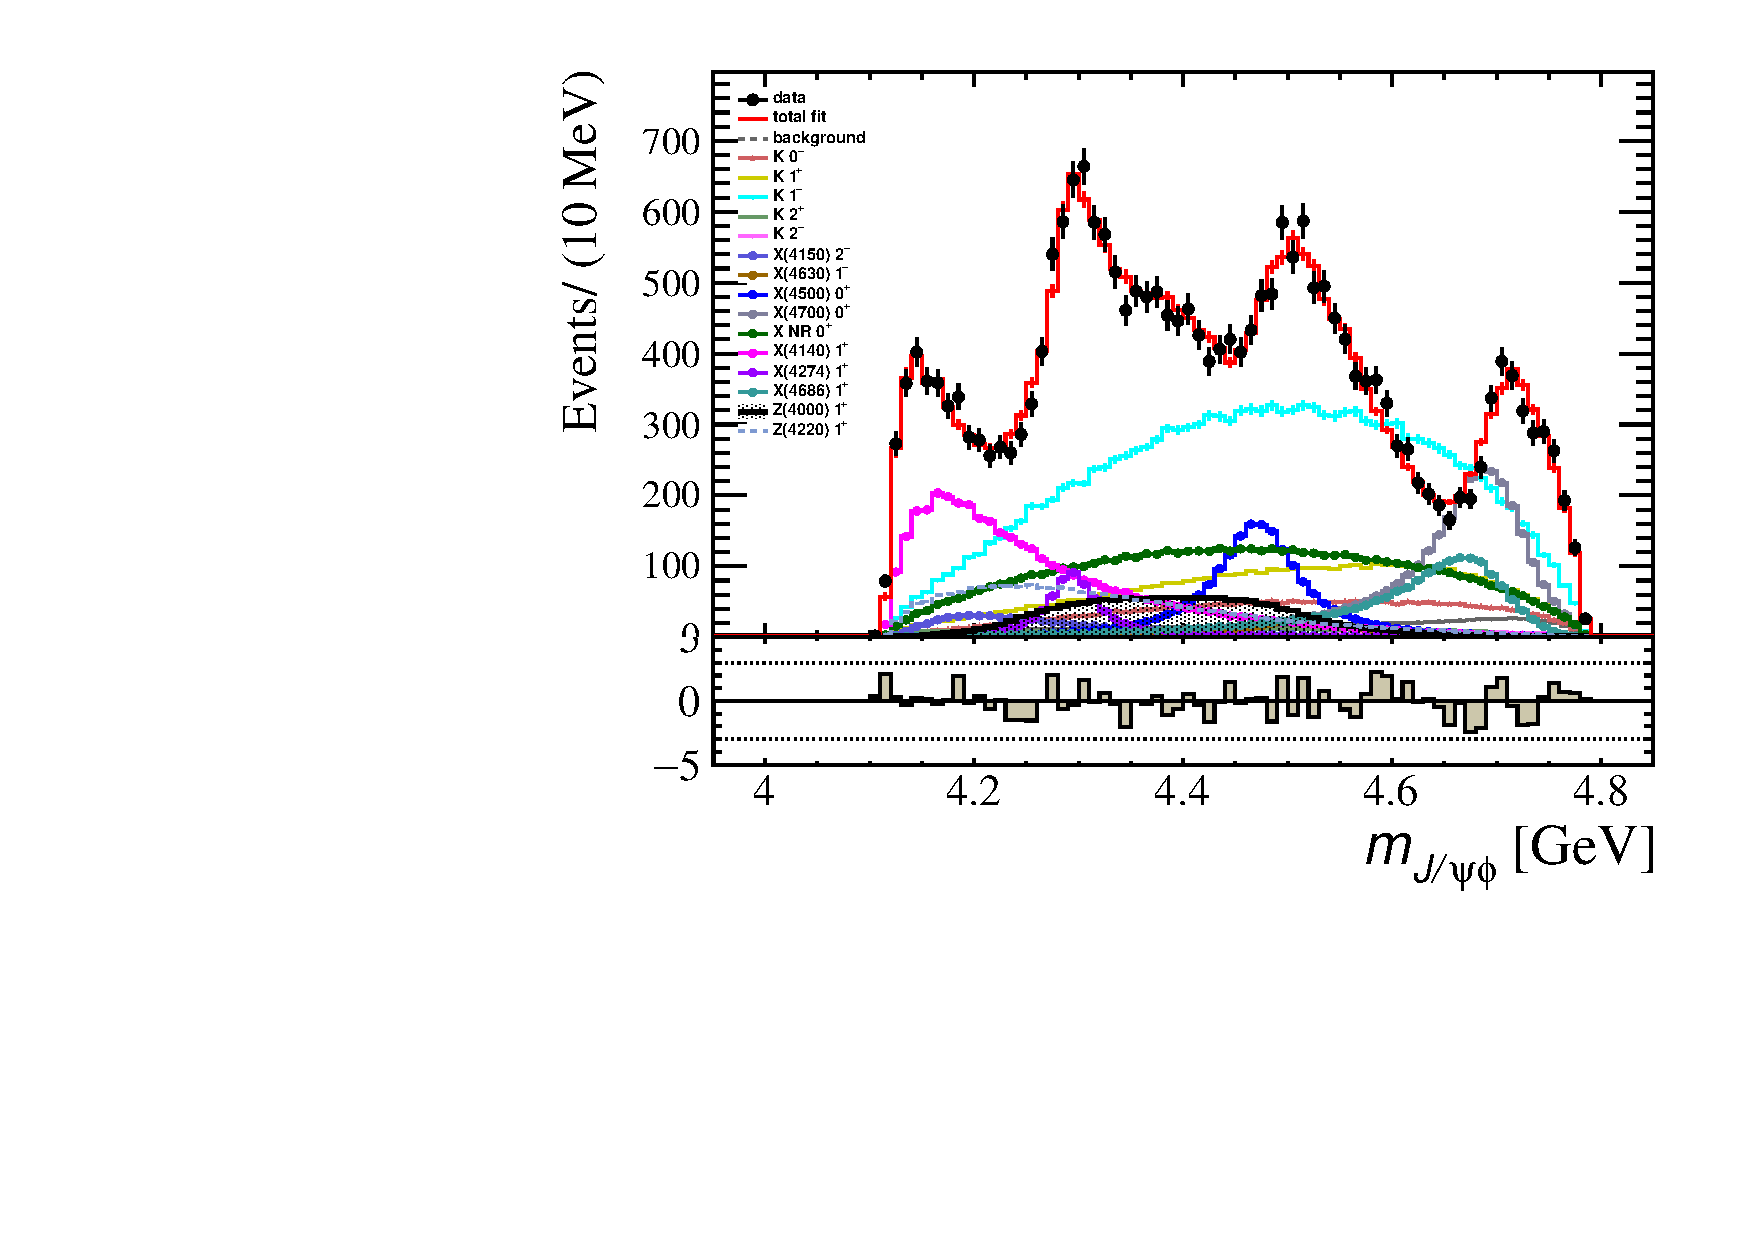
\includegraphics[width=0.33\textwidth]{Figures/03_Zcs/app_Kmatrix/mjpsiphi-X2mZ1PKM}
\put(-40,95) {\textrm{\small \bf(b)}}
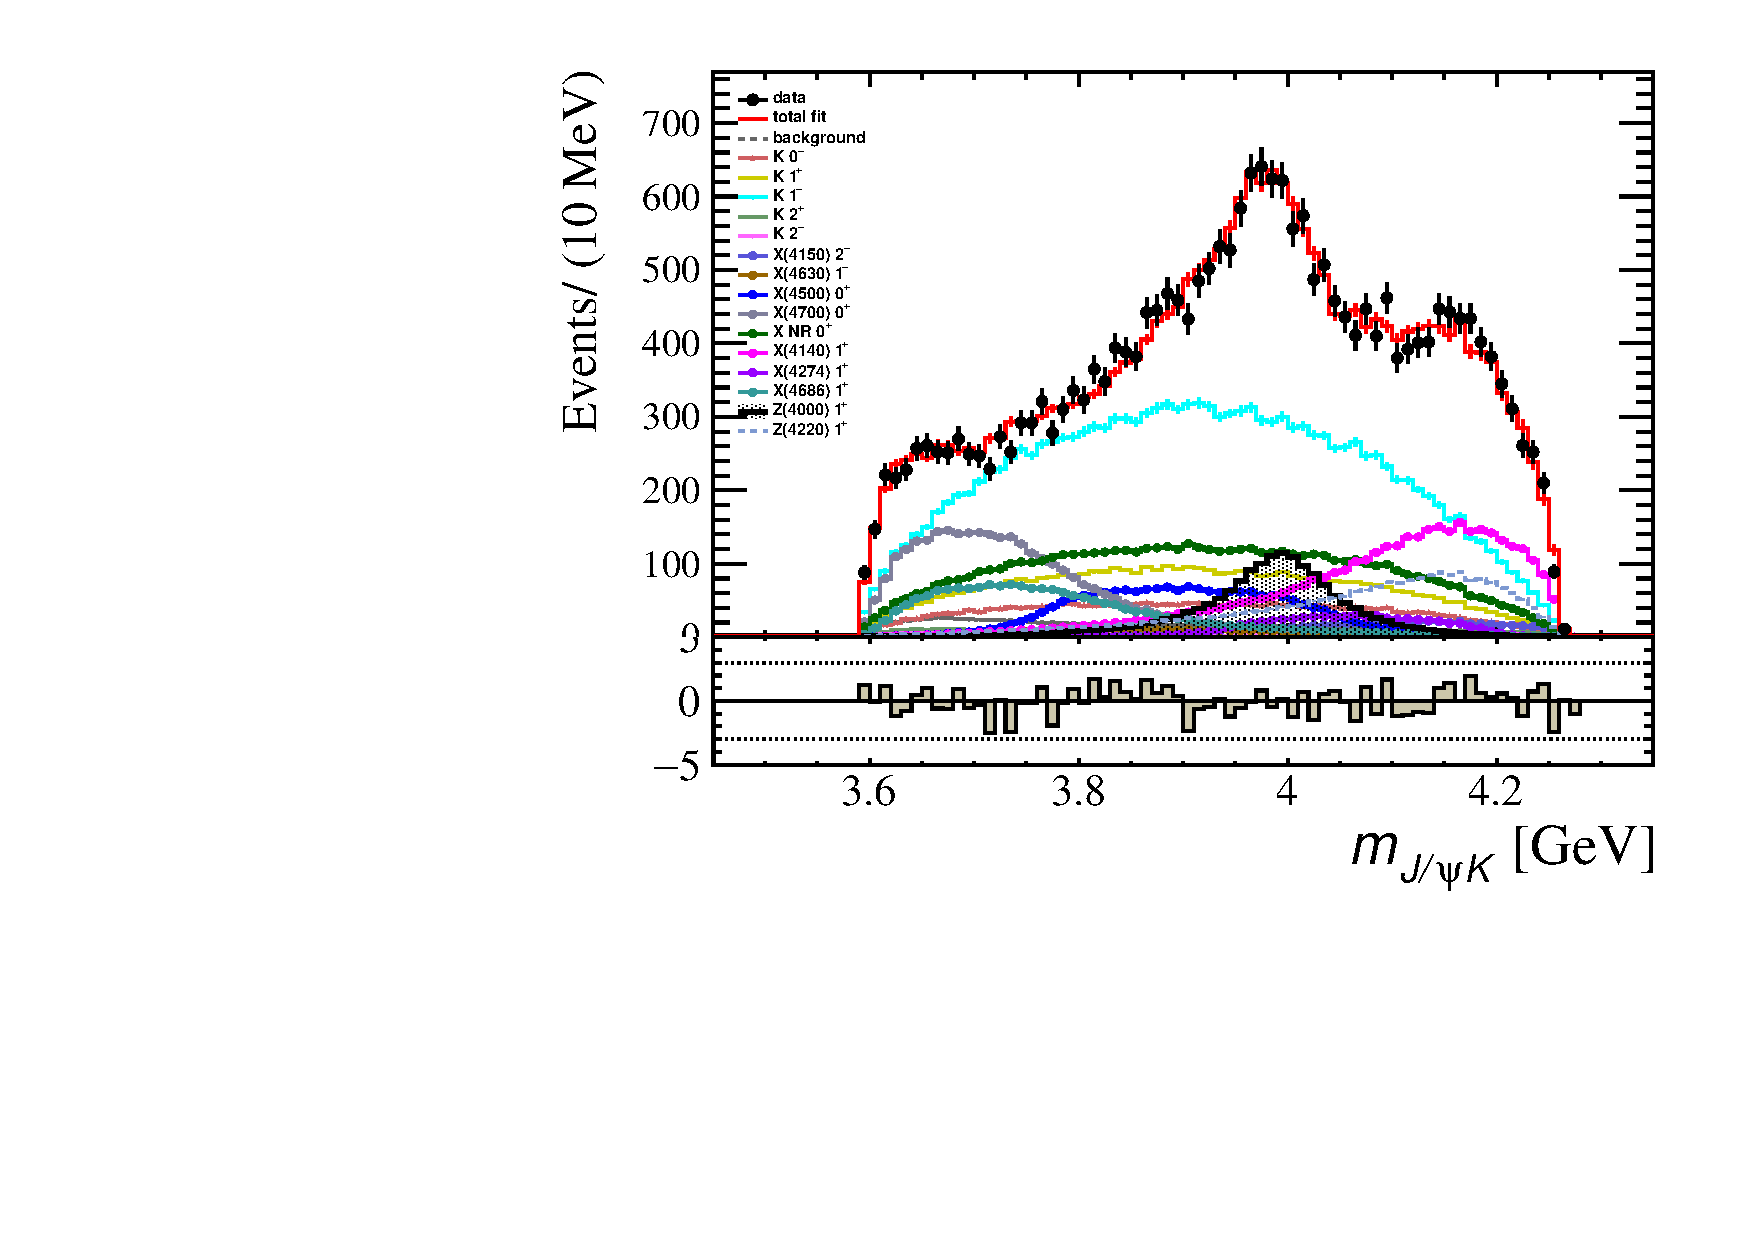
\includegraphics[width=0.33\textwidth]{Figures/03_Zcs/app_Kmatrix/mjpsik-X2mZ1PKM}
\put(-40,95) {\textrm{\small \bf(c)}}
\caption{Fit projections of (a) $\mfk$, (b) $\mjf$, (c) $\mjk$ from the nominal K+5X+2X+2Z model with K-Matrix for describing the $K^*$ resonances.}
\label{fig:fitKM}
\end{figure}

The KMatrix model with two coupling channels are tested, 
which are used to describe the $2^{1}P_{1}$ and $2^{3}P_{1}$ $K^*$ resonances, 
as the two states overlapping with each other.
And the detailed formula can be found in \cite{Henner:2020owh,PhysRev.126.360,PDG}.
We replace the BW to this model to describe $2^{1}P_{1}$ and $2^{3}P_{1}$ states, 
which overlapping with each other.
The floating value in the fitting includes resonance pole mass, 
coupling and physical background parameters.
We test this model in the nominal fitting, 
and the change of $ln(L)$ is around 10, 
which is pretty small.
The projections of this fit onto masses are shown in Fig.~\ref{fig:fitKM_More}.

\begin{figure}[!tbp]
\centering
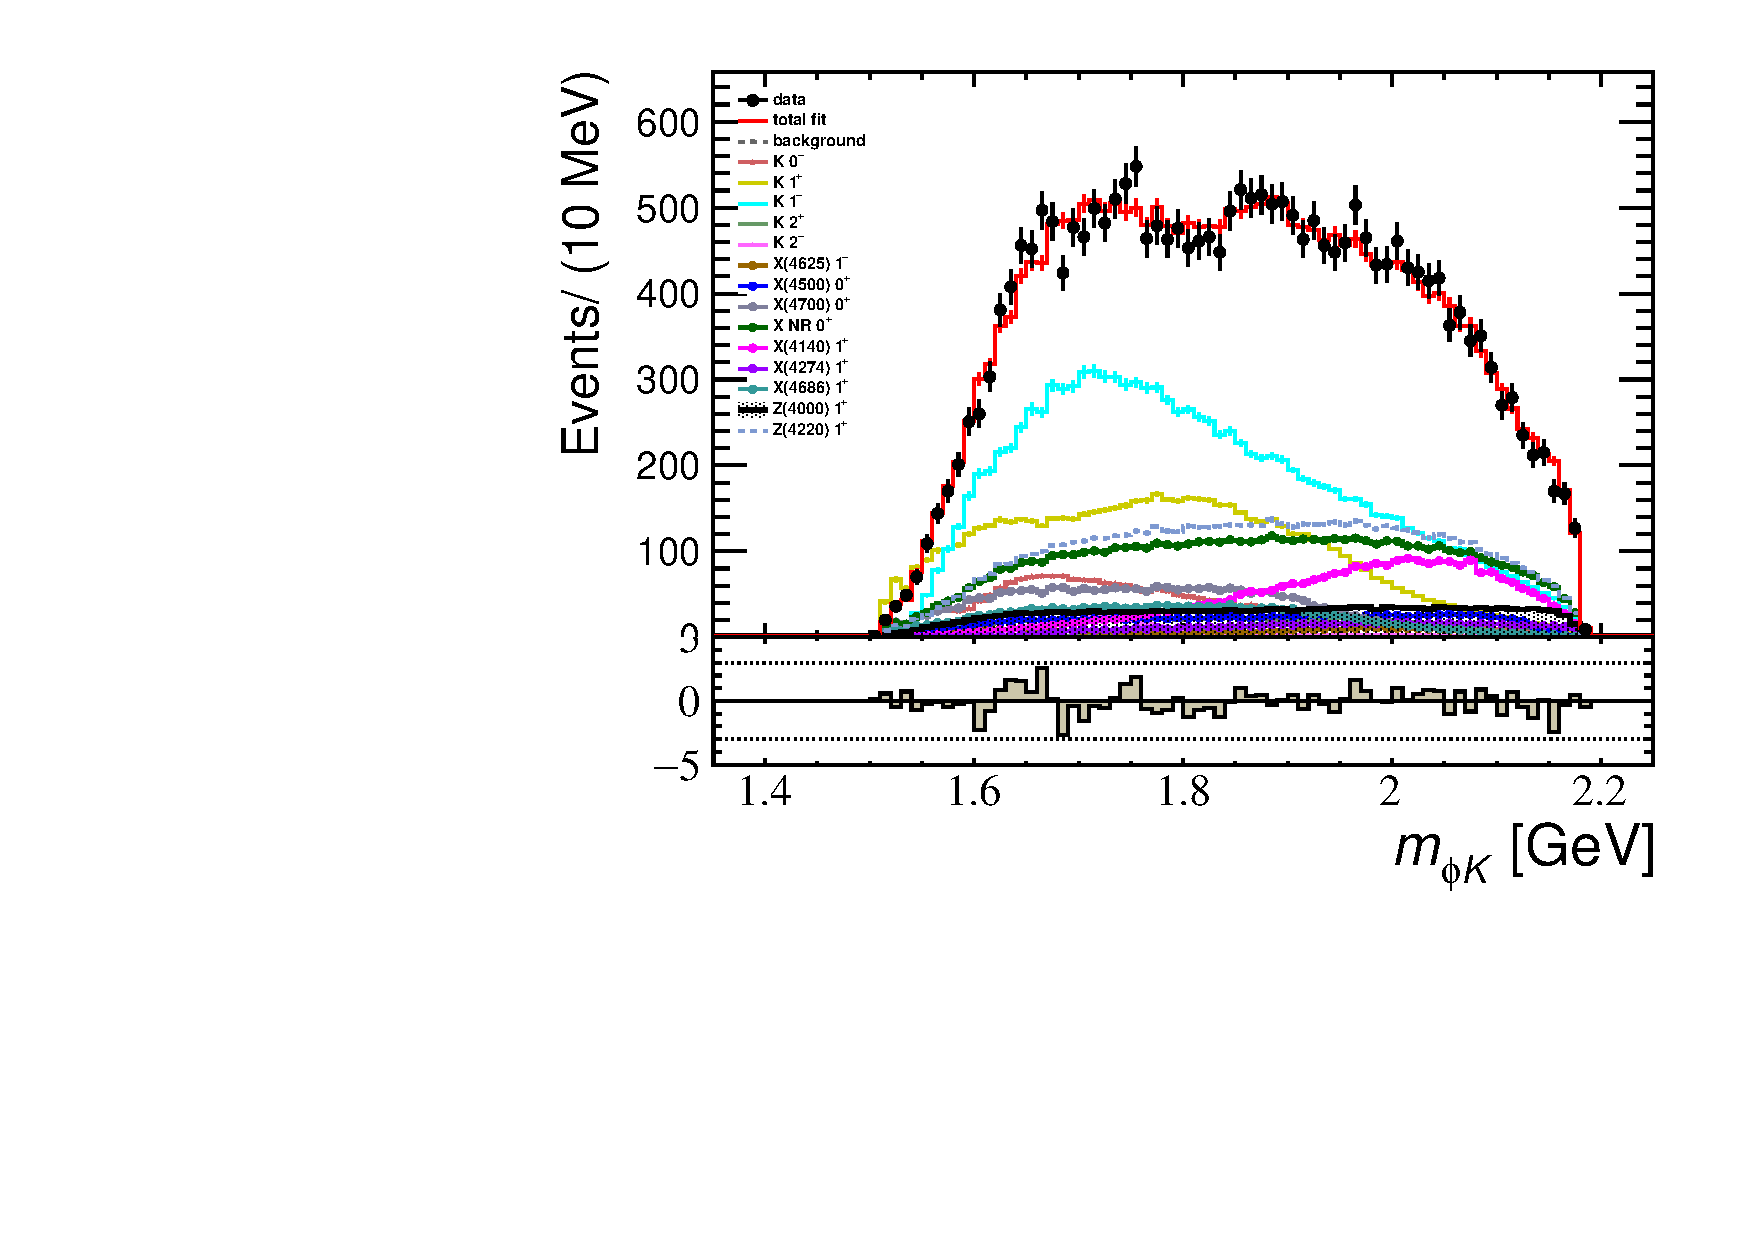
\includegraphics[width=0.33\textwidth]{Figures/03_Zcs/app_more_Kmatrix/mphik-GoodNew.pdf}
\put(-40,95) {\textrm{\small \bf(a)}}
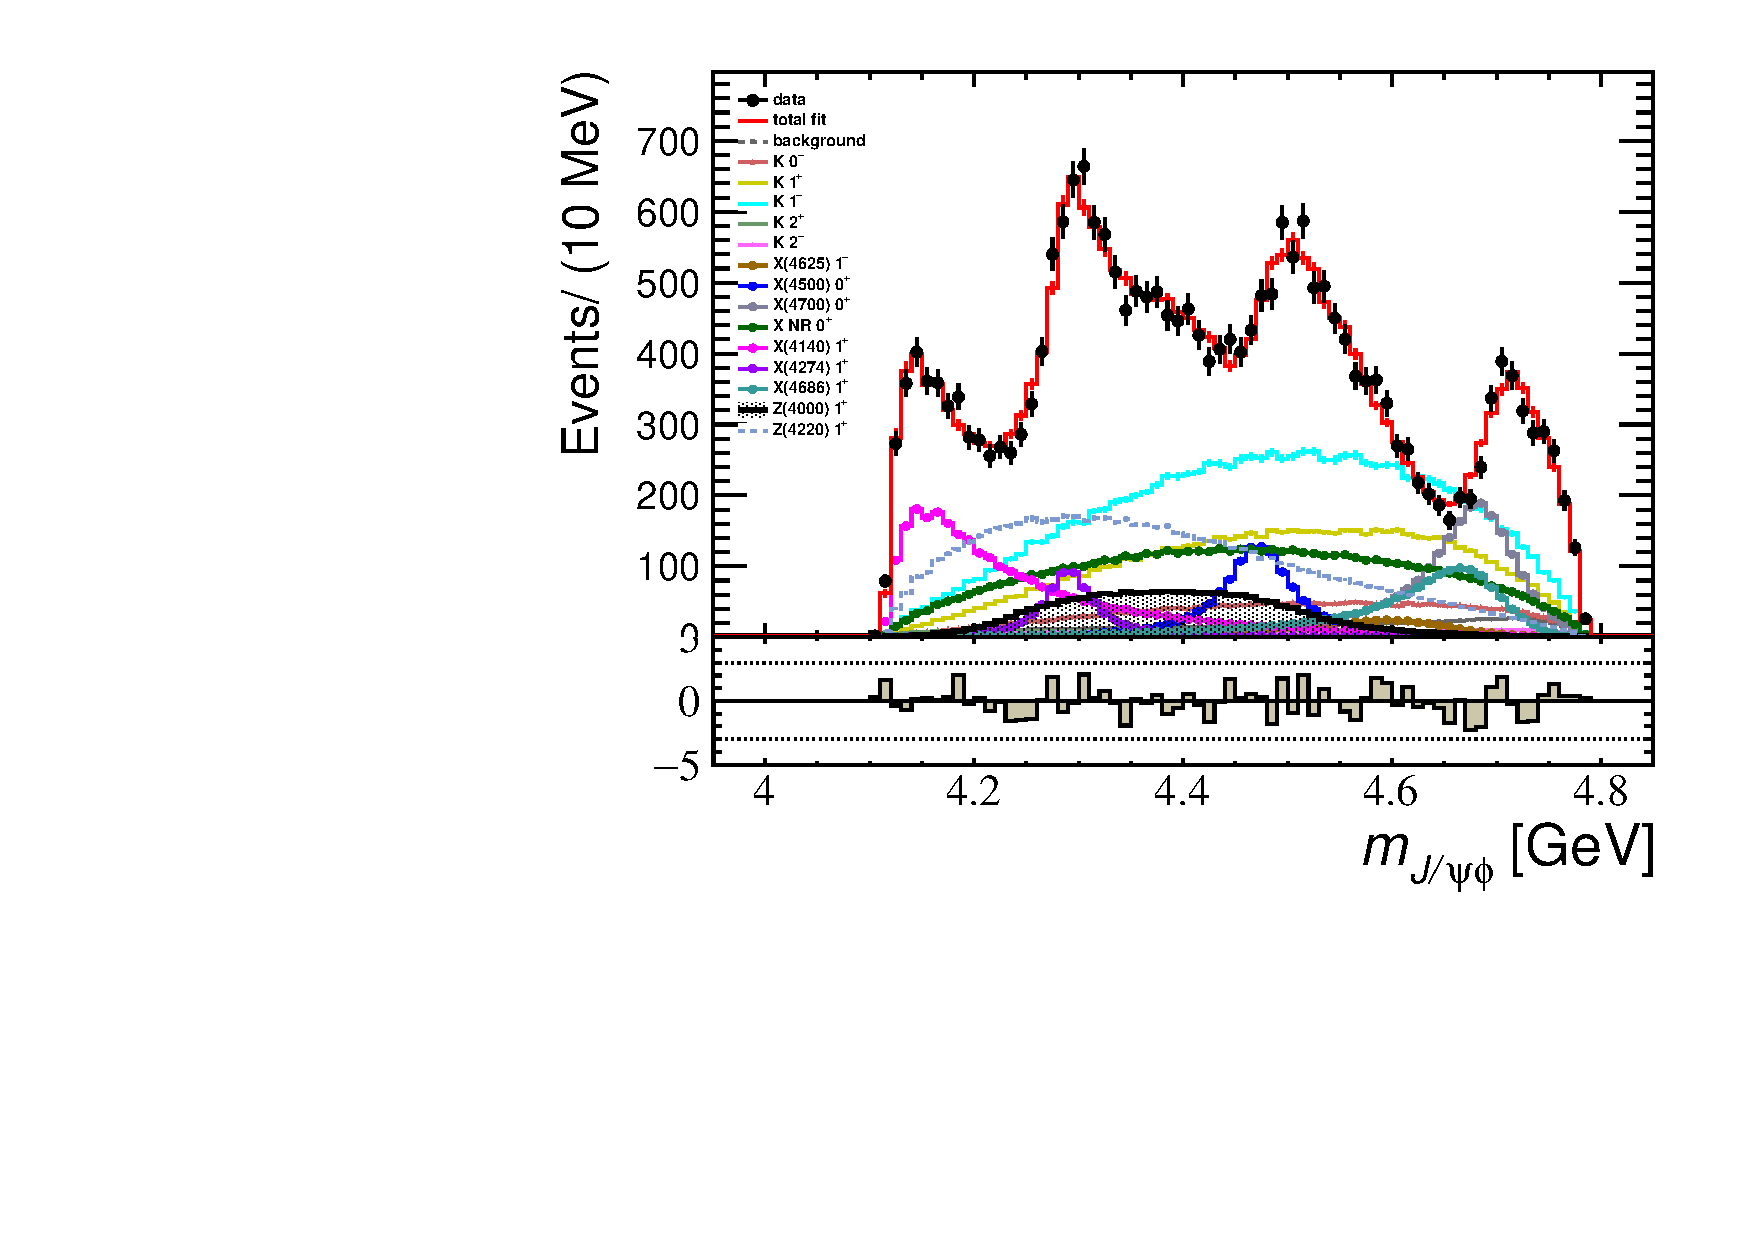
\includegraphics[width=0.33\textwidth]{Figures/03_Zcs/app_more_Kmatrix/mjpsiphi-GoodNew.pdf}
\put(-40,95) {\textrm{\small \bf(b)}}
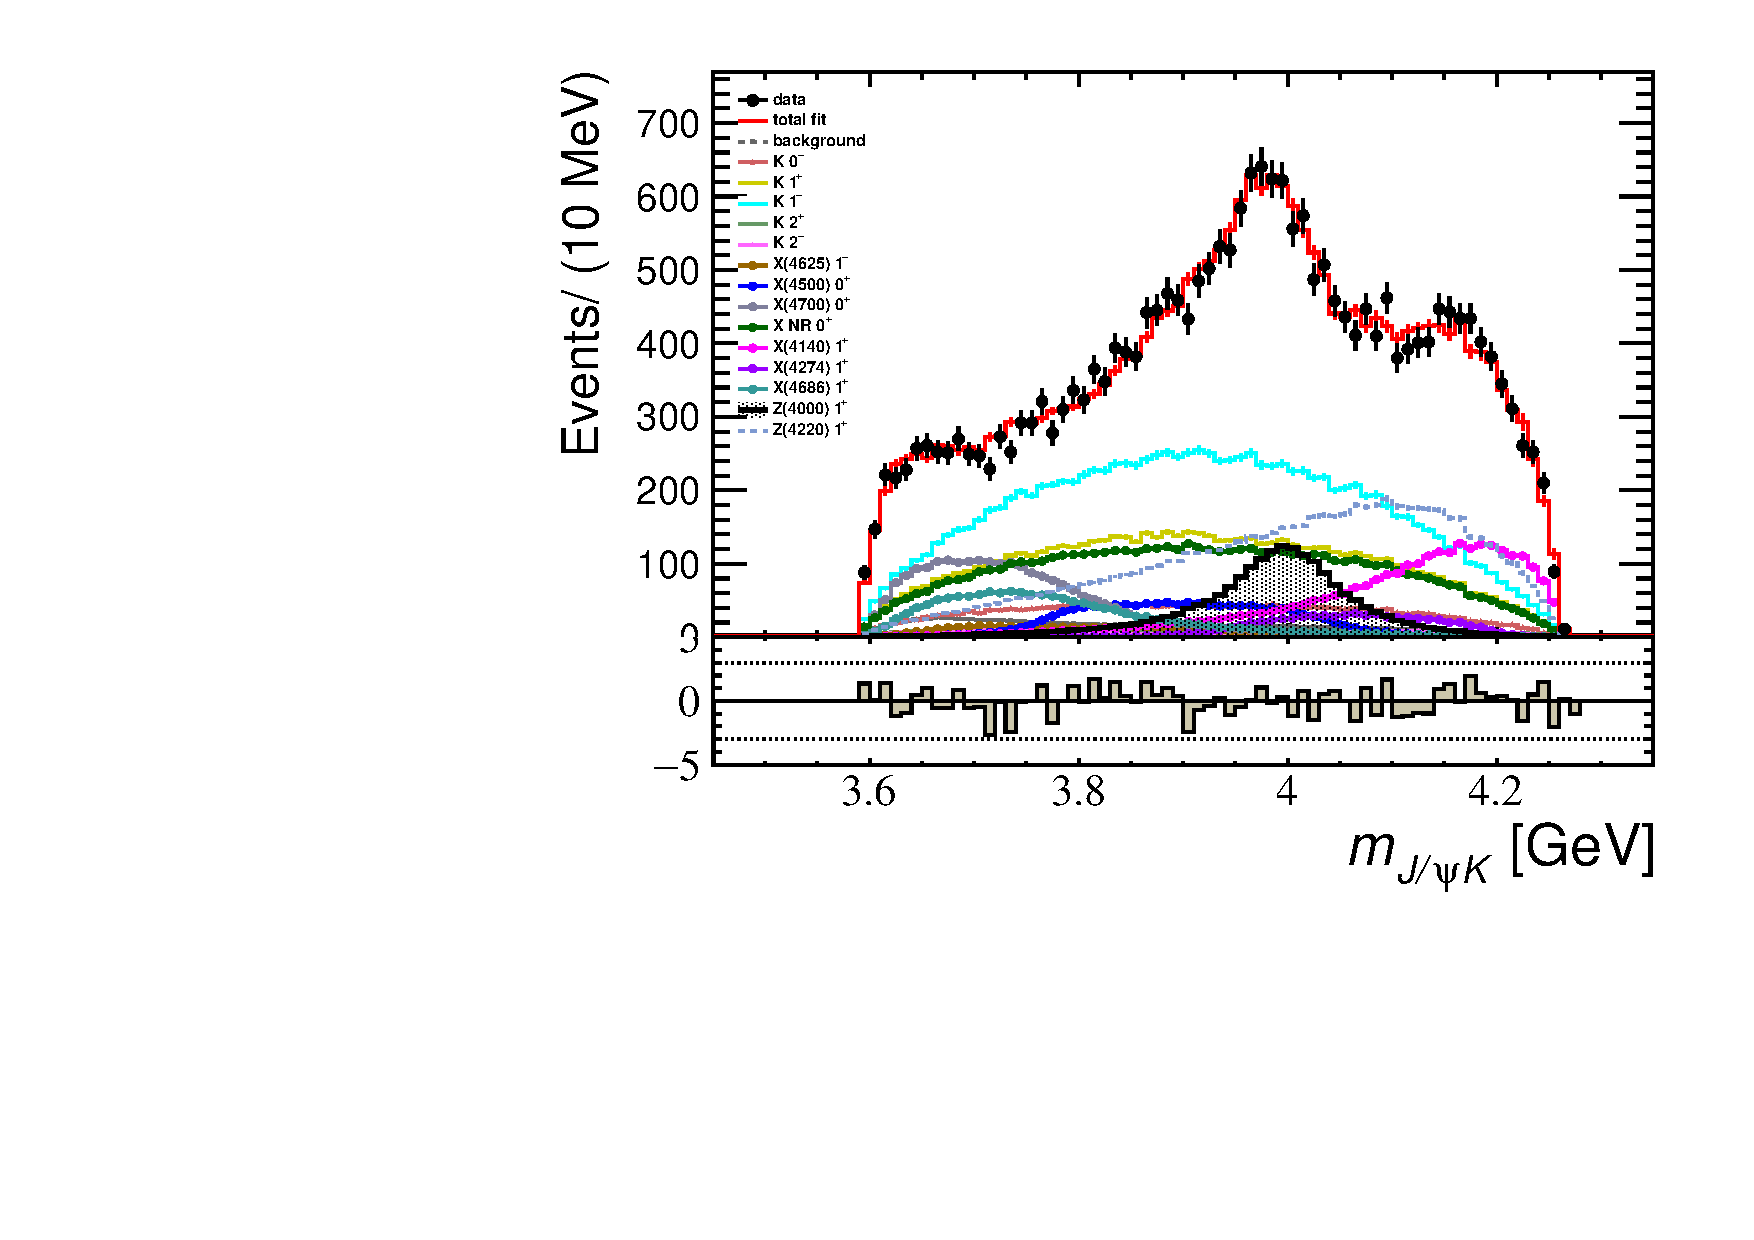
\includegraphics[width=0.33\textwidth]{Figures/03_Zcs/app_more_Kmatrix/mjpsik-GoodNew.pdf}
\put(-40,95) {\textrm{\small \bf(c)}}
\caption{Fit projections of (a) $\mfk$, (b) $\mjf$, (c) $\mjk$ from the nominal 2K(KMatrix)+7K+5X+2X+2Z model.}
\label{fig:fitKM_More}
\end{figure}




% vim:ts=4:sw=4
